\chapter{Agent-based modelling and economic theory \label{chapter:ABM}}

%Intro quote
\vspace{2cm}
%http://www.youtube.com/watch?v=wMFPe-DwULM
\begin{quote}
{\large
``When you explain a `why', you have to be in some framework that you allow something to be true. Otherwise you are perpetually asking why.''
\\
\hspace*{10cm}\emph{Richard Feynman\footnote{In interview on `Fun to Imagine,' BBC, 1983.}}}
}
\end{quote}

\begin{quote}
{\large
``How would you physicists like it if you had to survey a bunch of molecules to find out what they planned to do, only to have most of them change their minds anyway, and the government restructure the laws of physics because of some opinion poll?''
\\
\hspace*{10cm}\emph{`Gaz'\footnote{Comment at http://tamino.wordpress.com/2010/03/11/not-a-random-walk/#comment-40731}}}
}
\end{quote}

\vspace{2cm}


\section{Introduction to chapter \label{sec:ABMintro}}

This chapter introduces the concepts behind \gls{abm}. It also puts them in the context of ideas about modelling, concentrating particularly on those that have been developed in economics. The reason for this approach is to understand Richard Feynman's quote above: explanation requires knowing what framework the modeller is currently allowing to be true. This is an argument that goes back at least to Hume, who imagined a peasant and an artisan wondering why a clock had stopped. The peasant manages no better than `it does not go right'; the artisan knows more of the inner workings, and suspects the springs or the pendulum (\citealt{hume_treatise_1739} p.132 in \citealt{hoover_causality_2001} p.11). But while it is intuitively obvious, trying to work through its implications for model choices is less so. It is a tricky problem and as Friedman notes:

\begin{quote}
``There is no magic formula for wringing knowledge about complicated problems from stubborn facts. No method is proof against incompetent application.'' (\citealt{friedman_lange_1953} p.613)
\end{quote}

When discussing economic modelling, examples from the natural sciences present themselves as obvious thought experiments. This chapter uses plenty of them, and looks at arguments made by economists that do the same. A lot is written on the validity of such parallels; critiques of the utility-maximising foundations of neoclassical economics often go no further than pointing out its roots in Newtonian physics as self-evident proof of its absurdity (see section \ref{sec:abmlit}). But the quote above gets to the heart of the issue. Regularities in human behaviour do exist: how people react to cost changes is central to this thesis. But parallels with physics can only go so far. To pre-empt the conclusions, the argument for modelling people as predictable, reactive objects (perhaps with added noise) must be lightly made. It is unlikely that there will ever be the same robust link between levels of explanation in human behaviour as there are between atomic kinetics and gas theory (see section \ref{sec:levels}). Vriend quotes Lucas: economists are ``programming robot imitations of people, and there are real limits on what you can get out of that'' (\citealt{klamer_new_1984} p.49 in \citealt{hillebrand_artificial_1994} p.31).
%: it is a useful tool, as long as its limitations are kept in mind

The structure of the chapter is as follows:

\begin{itemize}
	\item An explanation of the basics of \gls{abm}, introducing \gls{oop}, discussing how it has come to inform model building, as well as the roots of the idea of `dependency';
	\item A brief overview of the \gls{abm} literature, setting the scene for the more specific argument that follows
	\item `Mapping the model', a section looking at how theorists from both economics and \gls{abm} points of view have understood how models should be built. The goal is to think through how to distinguish a good from a bad `mapping'.
	\item `Production and utility in an agent context' grounds the previous discussion by asking how agents with utility and production functions can be built.
\end{itemize}


\section{What is agent-based modelling? \label{sec:abmiswhat}}

In \gls{abm}, the `agents' are distinct code objects, programmed to interact with their environment and each other. \gls{abm} developed in tandem with \gls{oop}. Though \gls{oop} has a history going back to the sixties, it was not until the nineties that computing power and programming languages like Java developed enough to mark a `paradigm shift' in programming (\citealt{robinson_emergence_2009} p.211). This shift provided the soil for \gls{abm} to flourish. 

Writing in 2000, O'Sullivan and Haklay noted that \gls{abm} was ``a rapidly developing field that is already well beyond the scope of any limited survey'' (\citealt{osullivan_agent-based_2000} p.1410), a sentiment shared by one of the few authors brave enough to attempt an \gls{abm} textbook (\citealt{wooldridge_introduction_2009} p.xix). \gls{abm}'s use ranges from the most abstract artificial life to `autonomous' agents earning their keep controlling real-world infrastructure. As a field, \gls{abm} still seems as fluid and as expansive as it did ten years ago: little in the way of consolidation has taken place, despite pleas for standardisation and various groups arguing their particular framework offers a one-stop-shop for all things agent-based. 

Wooldridge defines objects as ``computational entities that \emp{encapsulate} some state, are able to perform actions, or \emph{methods}, on this state, and communicate by message passing'' (\citealt{wooldridge_introduction_2009} p.28). Objects are created from classes; a real-world metaphor would be that classes are the blueprint and objects the physical form. Thus, a model may have a single `Firm' class but many `Firms' created from that blueprint, with their own internal state.

This focus on objects' `encapsulation' - that `objects have control over their own internal state' - requires the programmer to think of them as separate entities, and to define relations between those entities very clearly. (The procedural element of programming has not gone away, however, and is still of vital importance, particularly with regard to timings; see section \ref{sec:timingstr}.) A popular online java tutorial (\citeyear{sun_what_1995}) has a simple illustration of encapsulation: if a rider of a bicycle attempts to change gear, the bicycle should have a `method' that ensures it cannot exceed its gear number. The rider is denied the ability to \emph{force} a gear-change above those available. In coding practice, this mean providing methods to raise and lower gears: the rider may \emp{`request'} a gear change, but the bicycle `decides' if it can be done.

The ideal of encapsulation leads to the idea of `loose coupling' (e.g. \citealt{jana_java_2005}): if objects can be built that rely is little as possible on needing to know how other objects function, code frameworks can be made highly flexible and reuseable. An example from the thesis model framework would be the data output code, where an earlier iteration hard-coded variable names to be stored. By providing the data store methods with a way to `read' variables from anywhere in the framework, target variables can be identified with a string name only rather than hard-coded - thus replacing a set of objects, one for each variable, with a single re-useable object.

However, as the introduction mentioned, the `dependencies' that loose coupling attempts to avoid presents some problems when used as a philosophy for mapping agent models to real-world features; this theme is taken up in section \ref{sec:mapping}.

Many of the coding innovations now associated with \gls{oop} that found their way into \gls{abm} have a prehistory in procedural programming. Some of these have become emblematic of the agent modelling ethos. For example, Thomas Schelling's segregation model, first presented in 1969 (\citealt{schelling_models_1969}) and later described in `Micromotives and Macrobehaviour' \citep{schelling_micromotives_1978} is often seen as the `Eve' of agent models (see, for example, Schelling's closing essay (\citeyear{schelling_fun_2006}) in volume two of the \gls{ace} handbook), and is used by Krugman as a compact illustration of how a good economic explanation links micro to macro results  (\citealt{krugman_self_1996}, p.15). Craig Reynold's `Boids', while originating from a desire to animate flocking, talked of agents as objects (\citealt{reynolds_flocks_1987}). Schelling initially used only pencil and paper (\citealt{schelling_fun_2006}); Reynolds used an \gls{oop} extension to LISP. 

These models pre-empted the later vital importance of encapsulation. In conjunction with a set of supporting \gls{oop} coding concepts, this has created a very powerful set of tools for defining how objects interact. This is not just of historical interest: it is hard to overstate the importance of the \gls{oop} paradigm's approach to the subsequent shape of agent modelling theory and practice. Section \ref{sec:mapping} examines this issue in depth. Before that, the next section gives an overview of \gls{abm}.

\section{ABM overview \label{sec:abmlit}}

\subsection{Agent-based computational economics (ACE) \label{sec:ace}}

This thesis uses agents to look for spatial economic outcomes from actors with heterogenous locations. There is very little in the way of `complex' behaviour, and where it does exist (for instance in the interaction of price-setting and production), it is not the focus of analysis. This is not to deny the uses of \gls{cas} theory. Evolutionary ideas are particularly important for developing an understanding of how economic growth actually functions (\citealt{martin_complexity_2007}, and see section \ref{sec:coord_production}), as well as the evolution of diverse market structures, rather than just postulating a `Market' (see e.g. \citealt{mirowski_markets_2007} discussing `marketomata'). But a perceived need to keep \gls{abm} and complexity umbilically linked cuts off some of the more mundane  - yet crucial - uses of heterogeneity. (Section \ref{sec:levels} looks at an example of an `argument from complexity' that illustrates this point.)

Otter \emph{et al.}'s agent paper presenting an economic geography model, for instance, argues it is possible to use ``complexity as underlying explanatory variable'' (\citealt{otter_abloom:_2001} p.1). If `complexity' can be used this way, so can `equations' or `statistics'. It is suggested that ``regional economics and geography'' are apparently ``not sufficient to explain the complex spatial patterns, such as clusters and sprawl, that we encounter'' (\citealt{otter_abloom:_2001} p.1). Their model is in some sense believed to be `validated' if it manifests some element considered complex. In another example, Boschma and Martin ask,``in what sense can complexity theory notions (or metaphors), such as the emergence, self-organisation, criticality and so on, be used to conceptualize the economic landscape?'' (\citealt{boschma_editorial:_2007} p.541) This is perhaps a natural consequence of some of the theories of explanation that have grown along with \gls{cas} theory; see section \ref{sec:generative} on Epstein.

As O'Sullivan and Haklay say, \gls{ace} is driven by ``a view of the `economy as an evolving complex system' promoted by the Santa Fe Institute'', accompanied by a ``widespread disillusion with neoclassical equilibrium economics'' (\citealt{osullivan_agent-based_2000} p.1412). Disillusion is a gentle term: the reality for some researchers is a rather more `year zero' feel, seeing \gls{cas} as ``a pioneering break from a moribund Newtonian worldview'' (\citealt{manson_simplifying_2001} p.412). Mirowski, for example, argues (paraphrased by Blaug) that ``the whole of neo-classical economics ever since the \gls{margrev} has been an attempt to create an economics that emulates all the essential features of of nineteenth-century physics.'' (\citealt{blaug_economic_1997} p.284) 

As Blaug notes, this is rather strong; there was no conscious attempt to emulate physics. Grauwin also points out that the economic interpretation is very different from the physical: ``scientific fields assume distinct points of view for defining the `normal' or `equilibrium' aggregated state'': physics uses entropy where economics has agents finding Nash equilibria and, as they note, ``the two approaches lead to radically different outcomes'' (\citealt{grauwin_competition_2009} p.20622). Nevertheless, from a \gls{cas} perspective, the faults with `traditional' economics are seen to be self-evident. What Conlisk calls the ``strange sacrifices required for the `ritual purity' of optimisation-only models'' (\citealt{conlisk_why_1996} p.686) are considered relics. While understandable at a time when no computers were available, the feeling is - as Mirowski says - economists should ``kick the habit of their physics envy and join the 21st century by rethinking the importance of computation and evolution in the way that they approach markets'' (\citealt{mirowski_kicking_2007} p.359). Edmonds goes even further, suggesting that numerical representation itself is questionable. For example, he criticises numerical representation of variety on the basis that not all the dynamics associated with variety (such as evolutionary dynamics) can be described numerically (\citealt{edmonds_against_2004} p.5).
%``what starts out as a working model or `proxy' for the phenomena ends up being mistaken for the truth about that phenomena'' (\citealt{edmonds_against_2004} p.5).

As section \ref{sec:spacesituate} discussed, \gls{ge} is descended from this `Newtonian' lineage. Unsurprisingly, then, there is very little overlap between the research agendas of \gls{ge} and \gls{ace}. \gls{ace} as a distinct sub-discipline of \gls{abm} takes it name from the broader school of computational economics. Despite arguments that \gls{ace} is perfect for re-examining the Marshallian roots of economics (\citealt{leijonhufvud_agent-based_2006}), it has tended to follow the `Santa Fe' research agenda. One editorial contains a good checklist of the concepts of this agenda: ``complexity, evolution, auto-organisation... emergence... bounded rationality, inductive reasoning'' (\citealt{consiglio_artificial_2007} p.vi).  

The economic coordination problem in particular lends itself to \gls{abm}'s default focus on interacting agents. Indeed, Tesfatsion defines \gls{ace} as ``the computational study of economies modelled as dynamic systems of interacting agents''. The natural question for \gls{ace} theorists thinking about markets is then: ``who does the job of the so-called market adjustment?'' (\citealt{consiglio_artificial_2007-1} p.102). This requires the modeller to ``analyze explicitly how agents interact with each other'' (\citealt{kirman_evolving_2001} p.460). Howitt, for one, sees this requirement as a key strength of the approach: ``one of the virtues of the \gls{ace} approach to economics... is that it forces one to make explicit the mechanisms through which individual actions are coordinated, for better or worse'' (\citealt{howitt_coordination_2006} pp.1068). Agents, it is hoped, force theorists to crack open the problem and look at the dynamics inside.
%underneath, and in doing so either validate or challenge equilibrium analyses. 

Hayek's short essay, `the use of knowledge in society' (\citealt{hayek_use_1945} p.529), is something of a talisman for this way of thinking. In particular, his strong aversion to macro-level assumptions fits \gls{ace} perfectly. He insisted that ``we must show how a solution is produced by the interactions of people each of whom possesses only partial knowledge'' (\citealt{hayek_use_1945} p.530) – articulating both an assumption that the `solution' arises from micro-level interactions, and that it must come from `boundedly rational' actors. Epstein's `generativist's question' (discussed in-depth in section \ref{sec:generative}) -  ``how could the decentralised local interactions of heterogeneous autonomous agents generate the given regularity?'' (\citealt{epstein_generative_2006} p.5) - echoes Hayek's take. Some theorists (\citealt{vriend_was_2002} p.2; \citealt{miller_complex_2007}) can imagine that, had Hayek only been able to access present technology, he would surely have embraced it, and complexity theory along with it.

This Austrian tilt to \gls{ace} is further reason for the lack of overlap with the kinds of questions \gls{ge} asks. A good example of how this manifests itself is the criticism levelled at the concept of equilibrium. As Blaug notes, ``the desideratum of any economic theory is the delineation of an equilibrium end-state'' (\citealt{blaug_trade-off_2009} p.224). These end-states are analysed in the same way that basic physical models of stationary systems assume all forces balance to zero and are then able to deduce force values required for that stationary state. In-keeping with the attacks on its Newtonian underpinning, Colander and Rothschild argue:
	
\begin{quote}
``the self-correcting `stability' vision cultivated by economic pedagogy is problematic in several respects. First and foremost, it is simply wrong: stability is not the norm in complex systems'' (\citealt{colander_sins_2010} p.286).
\end{quote}

Critiques of the equilibrium assumption predate \gls{abm}, of course. Holub made the case that any new framework would need to declare a `year zero': 

\begin{quote}
``The long tradition of equilibrium thinking in economics has lead to an unrivalled, consistent structure of thought... an anti-equilibrium attempt cannot build further on this structure, not even on the ruins of equilibrium theory (should it succeed in toppling this construction), it must on the contrary seek a new site for its own, a new thought structure, in other words, a new central idea'' (\citealt{holub_anti-equilibrium_1977} p.395). 
\end{quote}
% The framing of questions and the strategies towards their solution have been tried for a long time, concepts and methods are highly formalized and without logical contradictions. It is clear that such a logically well devised model has formed the structure and concepts of the models which have emerged from it...

Many seem to believe \gls{abm} is exactly this new central idea. The concept of the `Walrasian auctioneer', often a target of anti-equilibrium critics, is a good example of this in practice. It is described as an actual mechanism, though in Walras' own work it is used only as a thought experiment to explain the equilibrium outcome (\citealt{blaug_economic_1997} p.555-6). Many \gls{abm} theorists take issue with a centralised adjudicator capable of mediating a process of `groping' towards a set of market-clearing prices, and knowing the moment when they are all correct\footnote{See e.g. \citealt{tesfatsion_agent-based_2006} p.834, where it is argued that ``equilibrium values... are determined by market clearing conditions imposed through the Walrasian Auctioneer pricing mechanism; they are not determined by actions of consumers, firms, or any other agency supposed to actually reside within the economy''; see also Vriend (\citeyear{vriend_walrasian_1991}); \citealt{consiglio_artificial_2007-1}.}. The auctioneer concept is a good summary of everything \gls{ace} opposes as implausible. Once such convenient (but, it is argued, impossible) assumptions are shown to be unjustifiable, a Pandora's box is opened:

\begin{quote}
``The modeller must now come to grips with challenging issues such as asymmetric information, strategic interaction, expectation formation on the basis of limited information, mutual learning, social norms, transaction costs, externalities, market power, predation, collusion, and the possibility of coordination failure.'' (\citealt{tesfatsion_agent-based_2006} p.836)
\end{quote}

Each of these `challenging issues' does in fact garner plenty of attention from analytic economics: Stiglitz got his Nobel prize for his work on asymmetric information going back to the seventies (\citealt{rothschild_equilibrium_1976}), game theory deals with strategy (and `predation and collusion' are forms of strategy), and Krugman himself discusses expectation and the role of history  as a key element of his geographical work (\citealt{krugman_history_1991}). As regards agglomeration economies, the importance of externalities has been discussed in chapter \ref{chapter:location}. 

\gls{ace} models often share one vital feature with the equilibrium methods they reject, however: a market clearing point. This often means that auction-style models are used where markets reach a defined end-point via a bidding process – through many interactions, perhaps, but still terminating at the end of trade. An example would be Kirman and Vriend's fish market model, with an interdependent morning and afternoon's trading (\citealt{kirman_evolving_2001} pp.467). The question of what happens if markets do not `clear' was asked by Hicks, and Isard understood its implications for trade across space. If all actors are making market decisions on the head of a pin, an auction-style clearing market presents itself as the natural way to think about it. But as soon as actors have heterogenous location, that becomes impossible: `clearing market' conditions do not hold. From an \gls{ace} point of view, Dibble (\citeyear{dibble_computational_2006} p.1516) notes the effects of space on standard market-clearing assumptions. Ladley and Bullock also point out (\citeyear{ladley_strategic_2008} p.296) that market actors may be segregated by space, able only to interact with a given subset of others, and that spatial segregation forms natural networks as actors' ranges of interaction overlap. Hamill and Gilbert apply this idea `in reverse': they use actors with randomised location in an $R^2$ space, and a fixed radii around each actor determines their social network connections (\citealt{hamill_social_2009}, \citeyear{hamill_simulating_2010}). 

Leijonhufvud describes the nature of the kind of market that space imposes (though he is not discussing spatial economics). He quotes Hicks -

\begin{quote}
``In a normal, ongoing market, transactors are not all brought together in a single location and at the same time. Without centralisation and synchronisation, the supply-equals-demand condition `cannot be used to determine price, in Walras' or Marshall's manner'.'' (\citealt{leijonhufvud_agent-based_2006} p.1633; see also \citealt{ladley_effects_2007} p.83-4) 
\end{quote}

While easier to ignore this problem if geography is not an element of the model, one cannot consider spatially varied trade as `one market' (\citealt{isard_location_1956} p.43). Leijonhufvud makes another suggestion based on this, which he dubs `Marshall's laws of motion': that agents follow very simple rules in response to market changes, not be presumed to rely on a point on a supply/demand curve. For example, a consumer may say, `if demand price exceeds the market price, buy more' in the opposite case, buy less', or a producer may say, `if market price is above supply price, increase production; in the opposite case, cut back' (ibid p.1630). This basic idea is used for a key component of the transmission belt model in chapter \ref{chapter:connectedModels}, though with an important alteration. Consumers use only a constrained utility function; they do not use a `law of motion' at all. Producers do use a `law of motion' - but not to change production levels. Instead, they say, `if stock is more than my target, lower prices to sell more; in the opposite case, increase them to sell less'. This simple idea is the basis for producing a flexible spatial `general equilibrium.

It is the `non-clearing' part of this problem that the thesis model attempts to deal with, rather than the network element. Section \ref{sec:routedev} already made the argument that transport networks can be replaced with a Euclidean proxy when discussing distance, though only by acknowledging the severe limitations for discussing change this imposes. Ladley and Bullock note Wilhite making a related point: that if network change is slow compared to activity on the network, its structure becomes more important, not less (\citealt{ladley_strategic_2008} p.299 referring to \citealt{wilhite_economic_2006}). This thesis cannot answer this issue fully as it works within the Euclidean assumptions from section \ref{sec:routedev}, where it was argued that the success of Euclidean stand-ins is dependent on both the spatial and temporal scale under examination, as well as whether network dynamics are part of the research question. So the model cannot ask, as Epstein does, how ``the endogenous connectivity – the topology – of a social network affects its performance as a distributed computational device, one that... computes price equilibria, or converges to (computes) social norms, or converges to spatial settlement patterns such as cities?'' (\citealt{epstein_generative_2006} p.17-18). 

\subsection{Spatial versus economic agents}

A Venn diagram of \gls{ace} and spatial \gls{abm} would perhaps reveal just as little overlap as between \gls{ace} and \gls{ge}.  Torrens' recent review of `\gls{abm} in the Spatial Sciences' (\citeyear{torrens_agent-based_2010}) illustrates the point. One economic example picked up on is not actually about spatial modelling: Torrens cites Farmer and Foley's Nature piece who argue that the economy is complex, \gls{abm} can `do' complexity where equilibrium models cannot, representing something closer to reality; therefore, \gls{abm} is better:

\begin{quote}
``Agent-based models potentially present a way to model the financial economy as a complex system, as Keynes attempted to do, while taking human adaptation and learning into account, as Lucas advocated. Such models allow for the creation of a kind of virtual universe, in which many players can act in complex - and realistic - ways'' (\citealt{farmer_economy_2009} p.685-6).
\end{quote}

They suggest an effort akin to general climate modelling for the economy is in order, coupling the various social science disciplines in the same way climate models might couple ocean and atmosphere feedback. Their emphasis on  building a `virtual universe' is also present in many of the spatial models Torrens surveys (this idea is the subject of section \ref{sec:virtualworlds}). The cellular automata models surveyed by Torrens in particular have this quality. Crowd and `swarm' models loom large, leveraging the interactive properties of agents (a point noted by O'Sullivan and Haklay, \citeyear{osullivan_agent-based_2000} p.1411). 

In terms of spatial \emph{economic} models, Torrens cites his own work (among others)  - in one example, a technically rich implementation of a combined cellular-automata agent hybrid model (\citealt{torrens_geographic_2005}). There appears to be no driving research agenda, however, beyond proving the technical feasibility of doing so, though the ability of disaggregated models to produce `emergence and self-organisation' is mentioned (p.396).
%\footnote{He also mentions Krugman's `self-organizing economy' as containing an agent-based analysis – it doesn't.}

Agent models using explicitly spatial economic ideas that would seem familiar to a \gls{ge} theorist are few. Sasaki and Box  use \gls{abm} to attempt to `verify' classic spatial analytics like the von Thunen model (\citealt{sasaki_agent-based_2003}) by showing how the spatial equilibrium result can come about through individual-level action but, aside from referring to von Thunen himself, it sticks to the \gls{abm} literature. The work of Christopher Fowler stands out as a theoretically grounded agent model with the explicit aim of examining the \gls{coremodel}; this is discussed in-depth in the next section.

%But it is not only economic methods that are discarded; economic questions seem to have suffered the same fate.
\subsection{Fowler \label{sec:fowler}}

Christopher Fowler has attempted to recreate the \gls{coremodel} in agent form. This section discusses the two papers where he does this. In some key aspects, his goal is the same as this thesis. Specifically, he keeps the focus on the simple interactions:

\begin{quote}
``the effects of economies of scale, the role of preferences for variety in driving trade between regions, and the push/pull relationship between these two factors in shaping patterns of agglomeration and dispersal in economic activity based on transportation costs'' (\citealt{fowler_finding_2011} p.2).
\end{quote}

The title of his first paper – `Taking \gls{ge} out of Equilibrium' – indicates what Fowler initially thought an \gls{abm} approach should be good at: ``the inability of the deductive models to describe the movement of a system between equilibria represents a major drawback of these models'' (\citealt{fowler_taking_2007} p.267). An agent approach, he argues, is a good method for achieving this. In his first attempt, he set himself a specific goal: to ``re-create as exactly as possible the relationships in the economic [core] model'' (ibid p.266) in agent form, meaning that ``to the extent possible, the equations used to express the analytic model have been maintained.'' (p.272) His second paper made a few extra choices and aimed to ``explore the capacity of an economic system to identify a stable Nash Equilibrium without it being enforced by assumption.'' (\citealt{fowler_finding_2011} p.14)
%Nash eq reminder: everyone's found a strategy that they wouldn't want to change if they can see what everyone else is doing. 

%For instance, he keeps the final set of simultaneous equations outlined in section \ref{sec:coremodelapx}.
Fowler's direction of travel, then, is very much from the analytic core model towards agent modelling. The main conclusion from his first attempt was that -

\begin{quote}
``although the equations of the analytic model can be mimicked in a way that is sufficient for a simulation to run, such a simulation cannot be made logically defensible without significantly altering the relationships among workers, firms and cities posited in the analytic model.'' (p.282)
\end{quote}

In initially binding himself to the assumptions of the analytic core model, Fowler was stuck with one of the more thorny abstractions: there are no firms explicitly defined as separate actors. The equilibrium number of firms - a key feature of of the Dixit-Stiglitz \gls{monocomp} approach, as discussed in section \ref{sec:marketstructure} - is purely a consequence of consumer demand combined with \gls{lov}. As he puts it, ``firms appear and disappear in cities based on the full employment of the workforce even to the point of following the lead of workers who move from place to place in order to benefit from increased real wages.'' (\citealt{fowler_finding_2011} p.2) 

Fowler's first pass at an agent version of the core model, then, lacking any method for linking firm and consumer behaviour even implicitly, could not produce equilibrium firm levels. Fowler notes that ``as a result, the model fails to move towards any of the equilibrium conditions predicted by its analytic counterpart.'' (p.266) As he notes, the full `general' conditions present a fairly daunting proposition for the agent modeller: 

\begin{quote}
``the amount a firm can offer in wages is dependent on the amount it can produce and the price it receives for its goods. These quantities are affected, in turn, by consumer's wages, which depend on which firm employs them (and whether or not they have found employment at all.)'' (\citealt{fowler_taking_2007} p.277) 
\end{quote}

In this situation, how can actors, unable to coordinate through any central mechanism, produce stable spatial economic outcomes, especially given the extra new problems of an `absence of rational expectations' (p.275) stemming from actors' intrinsic inability to predict the actions of others? (This `true uncertainty' is discussed in section \ref{sec:abmprod}.) He also points out the uncertainty that firms face: they need ``some mechanism with which they could predict an appropriate production level for themselves and estimate the levels chosen by their competition in an environment where sufficient labour supply is not guaranteed. The delicate balance among the equations of the analytic model does not allow for the error and uncertainty that are necessary parts of this sort of prediction, and so a new set of relationships needs to be specified'' (p.282). 

In a statement he later appeared to regret\footnote{``Economists are largely willing to leave the exploration of the labour market to other models. Given the complexity of the model necessary to replace this assumption, this researcher, at least, has grown increasingly sympathetic to the allure of such a potent simplifying assumption'' (\citealt{fowler_finding_2011} p.7).}, Fowler goes on to say, ``as complex as this specification sounds, it is actually relatively simple in an agent-based framework where bounded rationality, learning by doing and other types of decision-making all have substantial supporting bodies of literature'' (ibid p.283).

There are two particular points to pick up on. First, to return to the need for explicit `firm' actors: it could be argued that the original \gls{coremodel} \emph{did} have firms – as part of an argument built on the \gls{monocomp} model. The fact that it did not have distinct firm \emph{agents} is what Fowler is criticising: he is arguing for what the next section calls a closer `descriptive mapping' – and, perhaps, that it is self-evident that any model without distinct `firm' objects is invalid. Certainly, it appears to be what he sees as the most unjustifiable simplification: ``geographical economics does itself a disservice by ignoring the labour market dynamics that are arguably the most important set of relationships driving the movement of labour and capital in the real world'' (\citealt{fowler_finding_2011} p.7).

The second point is the flipside of this: of course, Fowler must make his own simplifying assumptions. For example, he uses what could be described as a `localisation externality' simplification in the later paper's model. Three actions are taken: workers calculate their individual utility, an average utility level for each region is then worked out, and finally one randomly selected worker compares their individual level with the average between regions before deciding where will give them the better utility. The externality here is the regional average: each worker is allowed to `know' this value for all cities. This a necessary simplification for his purposes, but nevertheless not a dynamic that emerges from agent interaction.

Again, then, how does one tell the good simplifications from the bad? Which merely (in Hayek's phrase) ``assume the problem away and... disregard everything that is important and significant in the real world'' (\citealt{hayek_use_1945} p.530; see also \citealt{miller_complex_2007} p.87). The next section deals with this question.

\section{Mapping the model \label{sec:mapping}}

\subsection{`Descriptive' versus `functional' mapping \label{sec:code_vs_function}}

Miller and Page (\citeyear{miller_complex_2007} p.36) argue that one can construct a `homomorphism' between model and reality, an exact equivalence between identified real-world and model structures, but that too broad a homomorphism would be ``at the cost of lowering the model's resolution and value'' (p.40). As with arguments that models should aim for isomorphism\footnote{e.g. ``Isomorphism is a relation between mathematical structures. If there is a function that maps each element of one structure onto each element of another the structures are isomorphic'' (\citealt{downes_importance_1992} p.147). The term is used by, among others, Epstein to describe model-to-reality mappings (\citealt{epstein_generative_2006} p.24-5).}, these terms have particular mathematical meanings that encourage the idea that object structures should very explicitly map onto reality, and be transformable in the same way. They are too strict: the looser idea of `mapping' that Miller and Page start with can be a more useful way to think about building models. 

As Scott says, models and maps share a common purpose, both being ``designed to summarise precisely those aspects of a complex world that are of immediate interest to the map maker and to ignore the rest'' (\citealt{scott_seeing_1998} p.87). Baumol and Blinder conclude that modelling means choosing the best map – and that will depend on the purpose (\citealt{baumol_economics:_2005} p.12). Miller and Page point out it is intuitively obvious why a more realistic map may not be a better one (\citealt{miller_complex_2007} pp.36). Krugman takes this idea further: in the earliest Colonial explorations, map data consisted of verbal reports – sometimes apocryphal, spatially inaccurate, but still very useful (`six days south of the end of the desert you encounter a vast river flowing from east to west'.)  However, as more formal mapping took place, ``the improvement in the art of mapmaking raised the standard for what was considered valid data''. For a time, much useful information was lost (\citealt{krugman_fall_1993}). In the end, more accurate maps resulted – but in the transition to formalism and rigor, descriptive information gained may temporarily be lost. This is a map version of the streetlight effect: ``the methodology of economics creates blind spots. We just don't see what we can't formalise'' (\citealt{krugman_how_2008}).
%For Krugman, this is justified: ``a temporary evolution of ignorance may be the price of progress, an inevitable part of what happens when we try to make sense of the world's complexity'' (ibid). 
%Many theorists have described models as a kind of map; an abstraction that can help navigate the irreducible complexity of the real world

One of the supposed strengths of \gls{abm} is precisely that it promises to combine both descriptive accuracy and formalism, thus avoiding the streetlight effect. `Descriptive mapping' can appear a natural extension of the structure of \gls{oop}, which makes defining a close link between object structures and real-world counterparts an obvious thing to attempt. This is true both for objects themselves and the structural relations that \gls{oop} uses. For example, Tesfatsion uses \gls{oop}'s distinctions between public, private and protected methods to define private behaviours and to allow agents to ``communicate with each other through their public and protected methods'' (\citealt{tesfatsion_agent-based_2006} p.837). 

This section critiques this kind of `descriptive mapping' by looking at the reasoning of \gls{abm} theorists and more traditional economic thinkers, in particular Milton Friedman. The argument developed is that while \gls{abm}'s flexibility makes it appear feasible – and even desirable – to attempt `more realistic' mappings, the focus should be more on `functional mapping', where the function is closely tied to the purpose of the model.

Wooldridge notes from an early commenter a ``tendency to think of objects as `actors' and endow them with human-like intentions and abilities.'' (\citealt{next_computer_inc._object-oriented_1993} p.7 in \citealt{wooldridge_introduction_2009} p.28; see also \citealt{franklin_is_1996}). As regards structure, Tesfatsion argues that -

\begin{quote}
``encapsulation into agents is done in an attempt to achieve a more transparent and realistic representation of real-world systems involving multiple distributed entities with limited information and computational capabilities.'' (ibid p.838)
\end{quote}

It is an entirely understandable and intuitive belief: the closer the match between code and real-world - the more `realistic' - the better. But in what way should real-world systems be represented? It is obviously true that any effective model must in some way represent the dynamic it wants to examine; what Craik (\citeyear{craik_nature_1967} p.51) calls a `relation structure' (see \citealt{stafford_what_2009} p.3) and Suarez \emph{et al.} (\citeyear{suarez_scientific_2003} p.225) a `mapping of source to target'. But to what extent must this representation actually map directly? How important is `realism?' The goal is, as Hoover puts it, that - 

\begin{quote}
`` the idealised model capture the essence of the causal structure or underlying mechanism at work... Models are not, of their nature, cleanly idealised; they must involve particular properties, whose only function is to make them operable or realisable in a manipulable form.'' (\citealt{hoover_idealizing_2010} p.346)
% scientifically useful idealisation requires that
\end{quote}

Two examples of actual \emph{physical} models illustrate the point graphically. Craik argues that models ``need not resemble the real object pictorially; Kelvin's tide-predictor, which consists of a number of pulleys on levers, does not resemble a tide in appearance, but it works in the same way in certain essential respects'' (\citealt{craik_nature_1967} p.51). MONIAC, the Newlyn-Phillips hydraulic model of the economy, makes the same point. It was built mainly as an educational tool, using water to represent money-flows and various levers and wheels to control flows. Some argue it actually influenced some Keynesians (see \citealt{wood_john_1994} p.249). There were counter-arguments about the `misleading reduction of economics to hydraulics' (\citealt{shackle_years_1983} p.189 in \citealt{wood_john_1994} p.249). Newyln himself was well aware of this limitation: ``once the model has served its purpose... the student will need to return to the literature for the complications and refinements - hydraulics is no substitute for economics'' (\citealt{newlyn_phillips/newlyn_1950} p.119).

This is a perfect illustration for the upcoming section: one needs to know the purpose of the model before attacking it as misleading. The next section starts to unpick this issue by examining the place of both simplicity and realism in models.

\subsection{What role for simplicity? \label{sec:simplicity}}

The underlying motivation for descriptive mapping is, perhaps, that a perceived closer match to reality is its own `validation'. Conversely, this offers an easy line of attack for anyone unhappy with particular simplifying assumptions: they are unrealistic. But how can perceived lack of realism be used to judge a model, given that all models are simpler than reality? How to distinguish good from bad simplifications?

`Occam's Razor' is the idea that, given two theories that may explain some phenomenon, the simpler one is likely to be the better explanation. The centrality of complexity for \gls{abm} has tarnished the idea of simplicity, though the two should not really be opposed to each other. A particularly severe example of this sees \gls{abm} theorist Bruce Edmonds attacking Occam's Razor because `simplicity is not truth-indicative' (\citealt{gershenson_simplicity_2007}) He is very blunt about what simplicity should mean to modelling:

\begin{quote}
``if I am right, model selection `for the sake of simplicity' is either: simply laziness; is really due to pragmatic reasons such as cost or the limitations of the modeller; or is really a relabelling of more sound reasons due to special circumstances or limited data. Thus appeals to it should be recognised as either spurious, dishonest or unclear and hence be abandoned.'' (\citealt{gershenson_simplicity_2007} p.78)
\end{quote}

There are grounds for simplicity that go beyond laziness or dishonesty on the part of the modeller, however. Occam's Razor is not an `appeal' to simplicity, and Edmonds is right: simplicity by itself, is \emph{not} truth-indicative at all. Occam's Razor is a shortcut for finding successful theoretical needles in among the haystack of competing ideas. Friedman nicely outlines the role it has played in the physical sciences: ``the theorist starts with some set of observed and related facts, as full and comprehensive as possible'' (\citealt{friedman_lange_1953} p.282-3). There are, he argues, then an infinite number of theories consistent with the facts. Some `arbitrary' method is needed to choose between them - such as Occam's Razor. One could just as arbitrarily choose the more complex theory, but it so happens that simple explanations have done better in the physical sciences.

Plenty of the time, however, simple assumptions do not get tested in any meaningful way. These can sometimes be seen in the wild, appearing as `heroic assumptions'\footnote{One reviewer  of the English translation of Weber's `Theory of the Location of Industries' (\citealt{weber_theory_1909}) in 1930 warns, ``in approaching this book the reader must be prepared to meet a very abstract treatment and some very heroic assumptions'' (\citealt{fetter_review:_1930} p.233). There is a more recent example from Brakman \emph{et al.}, who see the same type of heroism underpinning the success of the \gls{dxs} (\citealt{brakman_new_2009} p.93).} in the literature. An heroic assumption is characterised by two things: being highly unrealistic, but opening up new avenues for analysis. As such, they have always been an easy target for critics, and \gls{abm} theorists have certainly taken aim at them.

Is there any way of telling what sort of assumption is valid? What distinguishes `heroic' from `useful' from `silly'? The next section looks at this question.

% The big question here, which I have written down somewhere. Tying to Feynman, to choosing your simplifications. Well, the argument is, it's not much good you giving me a mea culpa: yes, I know, the model has silly assumptions. You haven't then gone on to explain to me why or when that's OK. 

\subsection{What role for realism? \label{sec:realism}}

Moss and Edmonds' paper on `good social science' argues that:

\begin{quote}
``The essential feature of software agents devised for purposes of social simulation is that they should be validated as good descriptions of the behaviour and social interaction of real individuals or collections of individuals'' (\citealt{moss_towards_2005} p.10).
\end{quote}

They want a social science that ``coheres with directly observable evidence in as many ways as possible'' (ibid p.5). In seeking this coherence, they say that ``evidence and observation have priority over theory'' and ``when evidence and theory disagree the theory is changed'' (ibid p.4). Their goal here is to firmly fix the causal arrow from reality to theory and reject any approach that points in the other direction. As they put it:

\begin{quote}
``There are many such cases in the natural sciences where observation and experimentation lead to conceptualisation. We know of no such cases in the core of mainstream economics or sociology, where the conceptualisation has tended to come first'' (\citealt{moss_towards_2005} p.10).
\end{quote}

%Obviously, it would be madness to argue that reality is not the ultimate arbiter of theory.
In this view, valid theory must flow from reality by a process of accreted, validated induction. Theirs is only a subtle tilt in emphasis away from theory-building, but its impact on what counts as `valid' agent modelling is huge. It is suggested that Einstein's theories, built up from Maxwell's and a number of other theorists, embody the approach they espouse, being ``driven by experiment and observation of natural phenomena'' (ibid p.3). However, Einstein's view of the matter seems to have been rather different:

\begin{quote}
``Physics constitute a logical system of thought which is in a state of evolution, whose basis cannot be distilled, as it were, from experience by an inductive method, but can only be arrived at by free invention. The justification (truth content) of the system rests in the verification of the derived propositions by sense experiences. The skeptic will say: `it may well be true that this system of equations is reasonable from a logical standpoint. But it does not prove that it corresponds to nature'. You are right, dear skeptic. Experience alone can decide on truth.'' (Quoted in \citealt{kaldor_irrelevance_1972} p.1239.)
\end{quote}
%A. Einstein, Ideas and Opinions, New York, 1960, pp. 322 and 355 (quoted by Kornai, op. cit., pp. 9-10), q

The point here is not that `free invention' has free reign - `experience alone' still determines the truth-content of theory – but that reality does not automatically supply the descriptive elements of theory. 

The search for an understanding of gas theory (discussed below in depth) shows much the same role for `free invention' being thrown against the wall of reality. The many scientists involved went down different experimental routes, depending on prior assumptions about the nature of matter going back to Aristotle, and especially about atomism and whether a vacuum was possible. As Webster notes, for instance, Boyle got ideas about the elasticity of air from Descartes, who suggested ``air was analogous to a pile of wool fleeces'' (\citealt{webster_discovery_1965} p.445). Ultimately, reality was the arbiter of which theories were corroborated – and notice that reality provided the metaphor in this case - but induction never had the unique priority Moss and Edmonds want to give it.

Three issues flow from this. The first is whether social modelling \emph{needs} to meet the same criteria as physical modelling. The second, related, issue is what it should take to reject any particular theory as beyond the social-scientific pale. Any conclusive answer is beyond this thesis, but the above should at least give rather more slack to the use of Einsteinian `free invention' in model experimentation. Third is that, as regards realism, a straightforward `coherence' test of the sort quoted above would appear to be problematic.

In economic models, probably the most frequent subject of scorn is the idea that people are \emph{homo economicus}: infinitely rational utility-maximising machines. This serves as a good subject for thinking through the role of realism. Sociological critiques of \emph{homo economicus} abound: Hollis (\citeyear{hollis_rational_1975}; \citeyear{hollis_philosophy_1994} pp.52) takes on `rational economic man', and for Granovetter and Swedberg, the starting point of economic sociology is precisely that ``while interests are central to any explanation of economic activities, a purely interest-driven model is unacceptably distorted'' (\citealt{granovetter_sociology_2001} p.9). 

As mentioned above, a model is by definition simpler than the system it aims to represent. So what counts - in Granovetter and Swedberg's terms - as an acceptable distortion, and what is unacceptable? Moss and Edmonds' take is again a good representation of the starting point for many agent modellers. Talking about financial prediction (or lack of), they attack utility-based models: 
	
\begin{quote}
``The standard, na\"{\i}ve response... follows Friedman's classic claim that the descriptive accuracy of assumptions is irrelevant and all that counts is predictive accuracy...  its \emph{ceteris paribus} conditions fly in the face of common observation, common sense and experimental evidence.'' (\citealt{moss_towards_2005} p.9)
\end{quote}

Milton Friedman's argument - called the `F-twist' by Samuelson (see \citealt{blaug_methodology_1992} pp.91 for an overview) – is indeed a classic critique of the `basic confusion between descriptive accuracy and analytical relevance'. Friedman says that ``a theory cannot be tested by the `realism' of its `assumptions' '' (\citealt{friedman_essays_1953} p.23) Note, however, that he is not quite arguing assumptions are irrelevant. This idea has become something of a caricature – to the point where Moss and Edmonds can claim the argument is now `na\”{\i}ve'. Friedman makes an interesting case, however, and it is a very useful way into picking apart how models should map to real world. 

Friedman spends some time criticising ``necessarily unsuccessful attempts to construct theories on the basis of categories intended to be fully descriptive'' (ibid p.34). A model may succeed in `descriptive accuracy', but what about analytical relevance? It is true that Friedman focuses on prediction as the ultimate arbiter: 

\begin{quote}
``Complete `realism' is clearly unattainable, and the question whether a theory is realistic `enough' can be settled only by seeing whether it yields predictions that are good enough for the purpose in hand or that are better than predictions from alternative theories.'' (\citealt{friedman_essays_1953} p.41)
\end{quote}

A vital question is then: what is meant exactly by prediction? This is dealt with in section \ref{sec:prediction}. Before that, however, some context for Friedman's thinking. His argument is built on keeping clear blue water between a self-contained theoretical structure (like Einstein's take on physics as a `logical system of thought') and the problems it is used to analyse. For Friedman, theory in and of itself is nothing more than a tautologous filing system that, while internally consistent, by itself has no `substantive content' (\citealt{friedman_essays_1953} p.7): 

\begin{quote}
``The objective is to construct a language that will be most fruitful in both clarifying thought and facilitating the discovery of substantive propositions.'' (\citealt{friedman_price_1962} p.8)
\end{quote}

%This does not mean Friedman thinks assumptions are meaningless – only that t
Internal to any particular system, it does not make sense to single out any one element as an unrealistic assumption. They cannot, by themselves, be used to accept or reject a theory, because `everything depends on the problem' (\citealt{friedman_essays_1953} p.7). That includes whether or not something is an assumption: Friedman concludes, much as Blaug does, that ``the logical distinction between `assumptions' and `implications' disappears in a perfectly axiomatized theory'' (\citealt{blaug_methodology_1992} p.143). The two are distinguished from each other only by the particular question under examination. This does not mean, however, that Friedman thinks `assumptions are irrelevant'. As he says –

\begin{quote}
``if this were all there is to it, it would be hard to explain the extensive use of the concept and the strong tendency that we all have to speak of the assumptions of a theory and to compare the assumptions of alternative theories. There is too much smoke for there to be no fire.'' (\citealt{friedman_essays_1953} p.41)
\end{quote}

What counts as a `crucial' assumption will depend on the problem at hand, and is something that Friedman thinks is beyond the scope of any simple methodology to determine (ibid p.25). There are, in fact, situations where assumptions ``can be used to get some indirect evidence on the acceptability of the hypothesis in so far as the assumptions can themselves be regarded as implications of the hypothesis'' (ibid p.28). This will, of course, depend on the hypothesis being proposed. 

In a simple thought experiment, he suggests that one can state `leaves seek to maximise the sunlight they receive'. This is, of course, an egregious simplification of the processes a tree goes through to achieve that maximisation, but it is nevertheless ``more compact and at the same time no less comprehensive'' than a list of particular rules would be (\citealt{friedman_essays_1953} p.24). Friedman goes on to a human thought experiment: how one would go about modelling billiard players? A successful model – that is, one able to make good predictions of game outcomes, on average – might assume that they ``knew the complicated mathematical formulas that would give the optimum directions of travel, could estimate accurately by eye the angles, etc... could make lightning calculations from the formulas, and could then make the balls travel in the direction indicated by the formulas'' (ibid. p.21). Conlisk asks (discussing life cycle decisions):

\begin{quote}
``But what of a beginner taking the first shot, in poor light, on a badly warped and randomly moving table, with assorted friends and relatives guiding the cue stick?'' (\citealt{conlisk_why_1996} p.684)
\end{quote}

Then the assumptions would be poor ones for this situation: the model would not work.  A relevant thought experiment of Friedman's in this case goes as follows. The equation $s=1/2gt^2$ is a good representation of the way bodies fall under gravity (where $s$ is distance, $t$ time and $g$ a gravity constant). An assumption is that this happens in a vacuum: air resistance is left out. This leads to several examples where the formula fails: for feathers, or for objects dropped from thirty thousand feet. The point is – 

\begin{quote}
``... under a wide range of circumstances, bodies that fall in the atmosphere behave \emph{as if} they were falling in a vacuum. In the language so common in economics this would be rapidly translated into: the formula assumes a vacuum. Yet it clearly does no such thing.'' (\citealt{friedman_essays_1953} p.18)
\end{quote}

There exist only certain conditions where this simple model works, but that does not nullify its use in those conditions, and requires understanding the sort of error one might expect. 

In sum, Friedman's argument is run throughout with a strong vein of `it depends on the problem' and `nothing is set in stone'. Focusing purely on isolated assumptions makes it easy to dismiss (for example) \emph{homo economicus} as obviously wrong, but this is an error, stemming from a misunderstanding of the type of model-building Friedman argues to be useful. Later, section \ref{sec:rationality} examines the issue of utility in more depth, and looks at how the difference between assumptions and implications depends on what is being asked. Next, section \ref{sec:virtualworlds} looks at two model styles – `virtual worlds' and `engines of analysis' – and argues they closely resemble the distinction between descriptive and functional mapping. 

%The next section briefly outlines the different types of prediction.
%``what are regarded as axioms or postulates of a model from one point of view can be regarded as theorems from another, and conversely'' 26.
\subsection{Virtual worlds versus engines of analysis \label{sec:virtualworlds}}
%Leijonhufvud arguing for return to Marshall's questions... 
% http://delong.typepad.com/sdj/2011/05/milton-friedman-we-curtsy-to-marshall-but-we-walk-with-walras.html
% http://www.economictheories.org/2008/08/alfred-marshall-neoclassical-economics.html
%``the field seems to be retreating into a self-consistent but ultimately irrelevant approach (thus following the path of economics)'' (Edmonds, review in JASSS, 1. “Michael Wooldridge: Reasoning about Rational Agents”, n.d., http://jasss.soc.surrey.ac.uk/5/1/reviews/edmonds.html.)

Di Paolo \emph{et al.} contrast two positions on what simulations should be: ``maximally faithful replicas'' versus ``thought experiments: unrealistic fantasies which nevertheless shed light on our theories of reality'' (\citealt{di_paolo_simulation_2000} p.4). This argument in \gls{abm} has a strong parallel in economic comparisons between two nineteenth century theorists, Walras and Marshall. Friedman was a defender of Marshall's approach, saying consistently that he ``took the world as it is; he sought to construct an `engine' to analyse it, not a photographic reproduction of it'' (\citealt{friedman_essays_1953} p.35). Walras, in comparison, built what Blaug calls a ``a peculiar vision of a sort of `realistic utopia' '' (\citealt{blaug_economic_1997} p.569). He was the first theorist to construct a full `general equilibrium' model, in an attempt to work out how all elements of the economy managed to interact to produce an apparently stable outcome. (His use of the concept of tat\^{o}nnement or `groping' towards clearing prices has already been mentioned in section \ref{sec:ace}.) This approach became the foundation for arguments that such equilibria were also optimal. As Blaug notes, over time Walras displayed ``an increasing tendency...  to fit the world to the model rather than the model to the world'' (\citealt{blaug_economic_1997} p.569) – something carried on by further refinements to general equilibrium over time. Cast into modern language, Walras could be said to have created a `virtual world'.

A model's status as `virtual world' or `engine' is not an intrinsic property of the model itself, though via an accretion of theorists' choices, one or the other can become set in. As Friedman put it –

\begin{quote}
``... by slow and gradual steps, the role assigned to economic theory has altered in the course of time until today we assign a substantially different role to theory than Marshall did. We curtsy to Marshall, but we walk with Walras.'' (\citealt{friedman_essays_1953} p.89)
\end{quote}

%The \gls{coremodel} is a good example of how a model can act as both `virtual world' and engine. Maybe.

Building virtual worlds is sometimes an entirely reasonable goal. Weather models are an obvious example: the goal of meteorology is precisely to create as close a mapping as possible between virtual and real, where the virtual model can be played out faster than reality to make predictions about the future. But it is a mistake to think this is always a laudable, or even feasible, goal for human systems.

\gls{abm} is perhaps more structurally suited to virtual world building, insofar as it can be used to make simulacra that can appear to be worlds \emph{in silico}, but are these really different from the sort of virtual world Walras made? In \gls{ai} research, the `strong versus weak a-life' argument sees some saying virtual worlds can indeed be considered as more than just `simulations of living systems': actually `realisations of living systems'. Miller wonders whether, if the strong case were true, ``we would have to add a sixth kingdom of life to the current five... and databases of biological phylogenies would have to be updated every time a new Ph.D thesis in a-life was written'' (\citealt{miller_artificial_1995} p.21). It is hard to imagine this argument even arising in the same form for purely equation-based models – but \gls{abm} does not represent quite the break from purely mathematical methods that some claim. 

While computers are iterative by default (the system clock imposes a discrete structure), this does not necessarily mean that agent models \emp{must} be discrete, or indeed that they must be algorithmic: approximations to continuous and algebraic\footnote{Symbolic computing is capable of producing good analytic results: for example, where iterative approaches to integration like Runge Kutta functions can only approximate, symbolic computing can generally do as well as analytics in producing exact results where they exist.} functions are possible. \gls{abm}, however, has tended to integrate discrete time-steps into its approach, and methods are employed to design agent models with appropriate timing. 

It is true that \gls{abm} is algorithmic rather than equation-based\footnote{Epstein argues this distinction is logically false; see \citealt{epstein_generative_2006} p.27. Epstein argues all agent models must logically have an equation-based counterpart. In practice, however, this logical equivalence is less important than the way algorithmic and \gls{oop} approaches affect the choices modellers can make.}. While equation-based elements may be present (as they are in the thesis models) they are used by agents as part of their discrete decision-making. In a comparison of equation-based versus \gls{abm} methods for supply-chain management, Van Dyke Parunak \emph{et al.} highlight the fundamental differences. Equation-based methods using differential equations start with observables; in contrast, the \gls{abm} modeller -

\begin{quote}
`` - begins by representing the behaviours of each individual, then turns them loose to interact. Direct relationships among the observables are an output of the process, not its input.'' (\citealt{van_dyke_parunak_agent-based_1998} p.10)
\end{quote}

%It is easy to see the Hayekian bias towards distributed action here:
Again, this sounds like a virtual world: the `direct relationships among observables' can only be examined through a pseudo-empirical observation of the model as it plays out. In reality, there is less difference between equation-based and algorithmic approaches. Krugman's own work illustrates one aspect of this: it took him many years to work out what the full details and consequences of his modelling approach were:

\begin{quote}
``Why exactly I spent a decade between showing how the interaction of transport costs and \gls{increts} at the level of the plant could lead to the `home market effect' and realizing that the techniques developed there led naturally to simple models of regional divergence remains a mystery to me.'' (\citealt{krugman_was_1999})
\end{quote}

Part of the answer is that equation-based modelling can be just as opaque as \gls{abm}, and that working out the implications of the interactions is equally challenging. As Di Paolo \emph{et al.} note: ``in general, and qualified claims of the superiority of one style of modelling over another are not compelling.'' (\citealt{di_paolo_simulation_2000} p.3) Ultimately, however, the difference between virtual worlds and engines of analysis does not come down to their structure, but to the way they are interpreted by modellers. The one defining characteristic of `virtual worlds' is that they claim to explain something about this world purely through their own existence. It is taken to be self-evident that virtual and real world dynamics are identical in some key aspects. Arguments for model `realism' lend weight to this interpretation: virtual and real world dynamics are more alike.

A useful way to put some meat on the bones of this discussion is to examine an especially popular take on agent modelling, the idea of `generative' social science. Before that, the next section outlines three types of prediction: these will be used in the following sections to help shed light on the difference between `engines of analysis' and `virtual worlds'.

\subsection{Three types of prediction \label{sec:prediction}}

Three types of prediction can be defined. The first is forecasting: making a claim about something that will occur at a future point. The second is closely related, and uses precisely the same methods: in modern terms, it is `back-casting'. As Friedman puts it, prediction - 

\begin{quote}
`` - need not be forecasts of future events; they may be about phenomena that have occurred but observations on which have not yet been made or are not known to the person making the prediction.'' (\citealt{friedman_essays_1953} p.9)
\end{quote}

The third is what Betz calls `ontological prediction' (\citealt{betz_prediction_2006}). This is a claim about a phenomenon that has always existed (that has occurred, is occuring now, and will in the future) but was not known about or looked for. Einstein's work on the relationship of gravity and space, for example, describes something that always happened. The theory led Eddington to carry out his photographic test confirming that light `bent' near the sun as it followed a straight line in gravity-warped space. (See \citealt{almassi_trust_2009} for a recent discussion of this example.) Betz also notes the prediction of Neptune's existence from Newton's laws, which showed other planetary bodies' orbits to be incorrect without another planet to explain it. 

The discovery of tectonic plates is a more down-to-Earth example, and one used by Epstein (\citeyear{epstein_why_2008}). This example highlights the clear relation between the different types of prediction: understanding tectonic plates places a boundary around possible future outcomes that were unknown before. Earthquakes will mostly happen on or near lines of tectonic plates, and understanding of tsunamis can also be built on that knowledge (\citealt{thompson_contra_2009}, who critique Epstein's approach).

`Ontological predictions', then, can lead to discoveries, if the predictions are good, as well as provide methods for placing bounds around forecasts. Putting it in `streetlight effect' terms, they shine a light into previously dark areas. Krugman's \gls{coremodel}, it could be argued, is an economic example of this, opening up novel ways to think about international trade that do not rely on factor differences, as well as enabling a much more clear conception of the possibility of emergent `core' and `periphery' structures. If a theory can facilitate the `discovery of substantive propositions', these may take the form of ontological predictions.

%but it also highlights the flipside of ontological predictions. Prior to Krugman's work, trade models could not account for intra-industry flows...
\subsection{Applied versus theory \label{sec:appliedvstheory}}
%Argument: that the distinction between applied versus theory links to `virtual worlds versus engines'... because?
%Well: blurring, but that doesn't really seem to apply to economic VWs. Maybe I shouldn't over-egg that particular pudding. 


Webber, writing in the eighties, identified some confusion from mixing up the purpose of models. He distinguishes between applied and theoretic (or `scientific') models (\citealt{webber_explanation_1984}). Theoretic models are ``designed to increase our understanding... and to integrate theoretical and empirical research.'' Applied models, in contrast, are tools used in the day-to-day running of organisations and institutions, and in longer-term forecasting and planning. They  - 

\begin{quote}
`` - regard the form of society as given and are produced to make that society operate more profitably; since scientific research examines the conditions under which the society operates and the manner in which it is changing, such research ought not to regard the form of society as constant.'' (p.149)
\end{quote}

Webber argues this comes to down to `a difference between the need to understand and the need to prescribe' (p.151). Traditionally in economics, this is the distinction between positive and normative analyses (\citealt{friedman_essays_1953}). 

Questions from an applied or theoretic perspective are completely different. Transport economics is a good example of an applied approach; as Button says, it takes a ``given land-use pattern and looks at methods of providing efficient transport services within this constraint" (\citealt{button_transport_2010} p.51). He also notes the same `applied' ethos, taking existing structures as given in the short-term, characterises supply chain analysis and operations research (ibid p.327). Compare this to Haggett's search for a `comprehensive model of route development' discussed in section \ref{sec:routedev}: a transport economist may need to consider, for example, how the risk from fuel cost changes could be mitigated through infrastructure design, but that is quite different to asking, how would the spatial economy as a whole be affected by these cost changes in the long term?

\gls{abm}, as with any form of social modelling, has feet in both camps, but the boundaries between them are more blurred than were the urban models Webber examined. Some do identify a similar distinction; for instance, Brown and Xie (\citeyear{brown_spatial_2006} p.941) talk of two `modes': instrumental and representational. Instrumental agents are carrying out some real-world task, whether collecting information on the internet or optimising container port flows, whereas representational agents are doing just that: representing some object. But these do not seem to count as either `applied' or `theoretic': either can be used in applied settings, and either could have a role in operations-related work. Optimisation of container ports is a typical case. The gap between models of good flow and reality is shortened; the model not only represents the target system, it is uploaded directly the port's computer systems, in effect making the model reality (\citealt{steenken_container_2004}). If models are maps, these maps are reflexive: it not only describes, but is used to act upon the world (\citealt{scott_seeing_1998} p.87). 

The need to model systems that require regulation is not new; Conant and Ashby (\citeyear{conant_every_1970}), for instance made an early argument for this. One might reply that agent-based operations models are qualitatively different, because cognitively more sophisticated. Regardless of whether this is true (and some cyberneticians would probably disagree; see e.g. \citealt{beer_brain_1994}), there are other reasons why the distinction between applied and theoretic models has become blurred in \gls{abm} that tie back to the type of mapping a model is meant to achieve. 

This mirroring of real and virtual systems is underpinned by arguments that, as Epstein says, ``certain social systems, such as trade networks, are essentially computational architectures.'' (\citealt{epstein_generative_2006} p.16) Epstein can thus develop a theory that computations carried out \emph{in silico} can be considered as a version of the physical computation under study. Similar lines of thought about theoretic agent modelling have created quite a tangle as regards the model-reality relationship. For instance, an argument has developed that such models can actually be ``synthetic sources of empirical data'' (\citealt{di_paolo_simulation_2000}, who criticise this approach). In combination with the idea of `emergence', this has been followed through to its logical conclusion: what Epstein calls `generative social science', in which a model that generates a particular phenomenon can be said to explain it. 
%(Epstein's case is discussed in more depth below, in section ref{sec:generative}.)

\subsection{Generation versus explanation \label{sec:generative}}

Joshua Epstein's work on `growing artificial societies' (\citealt{epstein_growing_1996}) first presented his notion that \emph{in silico} emergence could be a form of explanation in and of itself. The motto became, `if you didn't grow it, you didn't explain it' (\citealt{epstein_generative_2006} p.xii). Epstein calls this `generative explanation' and styles himself has a `generativist.' He sees computational models as `a new scientific instrument' (ibid. p.xv) able to generate explanations about the social world almost without reference to physical reality. This stems from the idea that both `worlds' are in some sense producing the same dynamic. As Epstein puts it, ``the agent-based approach invites the interpretation of society as a distributed computational device, and in turn the interpretation of social dynamics as a type of computation'' (ibid. p.11). Epstein (perhaps accidentally) gives a perfect illustration of the blurring between virtual and real worlds this argument leads to: 

\begin{quote}
``No-one would fault a `theoremless' laboratory biologist for claiming to understand population dynamics in beetles when he reports a regularity observed over a large number of experiments. But when agent-based modellers show such results – indeed, far more robust ones – there's a demand for equations and proofs.'' (\citealt{epstein_generative_2006} p.28)
\end{quote}

They might fault them, however, if they claimed their experiments had in fact explained the behaviour of beetles in the wild. More than that, there are plausible reasons for thinking live beetles might be a better model than an artificial life version, even in a laboratory setting. No-one would fault them for using either digital or live models to explore the problem – but this is a much less grandiose goal than explanation. Yet for Epstein, any model `sufficient to generate' a target macroscopic phenomena has succeeded in explaining it. This may be in part hyperbole, since it appears to be contradicted by statements elsewhere (see below), but it is still striking. 

Epstein picks on the central dogma of neoclassical economics, discussed in section \ref{sec:ace}, as a basic illustration of his argument: demonstrating the existence of equilibria says nothing about the process of reaching it. Epstein says of equilibrium -

\begin{quote}
``To the generativist, this is unsatisfactory; to explain a pattern, it does \emph{not} suffice to demonstrate that – under this ensemble of strictures – \emph{if} society is placed in the pattern, no (rational) individual would unilaterally depart. Rather, one must show how the population of boundedly rational (i.e. cognitively plausible) and heterogeneous agents... could actually arrived at the pattern on time scales of interest'' (ibid. pxiii).
\end{quote}

The generative approach, then, sounds very Hayekian: ``it is irrelevant that equilibrium can be computed by an economist external to the system... The entire issue is whether it can be attained – generated – through decentralised local interactions of heterogenous boundedly rational actors'' (ibid. p.27). 

Schelling's segregation model, discussed by Epstein as a classic model of emergence, illustrates the problem of privileging this kind of `generation'. As a virtual world, one makes the conclusion Epstein does: it `explains' segregation, and the model's use stops there, `brushed under the carpet of emergence' (\citealt{di_paolo_simulation_2000} p.8). As an engine of analysis, it presents a hypothesis: a possible dynamic factor, among others, that may explain something about real-world segregation. Putting aside the hidden assumption - that all social macro phenomena must be the result of a process of interaction between micro-elements – it would need to be put into the context of a fuller theory, that might include (for example) the racial impact of transport infrastructure (e.g. the policies of Robert Moses, see \citealt{winner_artifacts_1980}), regeneration policy (\citealt{gaffikin_community_2011}) or the effect of estate and letting agents' steering (\citealt{phillips_race_1992}). 

A last example gets to the nub of the issue with the generative approach. Epstein considers the `confusion between explanation and description'.  He looks at an example from his `Sugarscape' models (\citealt{epstein_growing_1996}) where agents generated a sine-like oscillation of population change over time, and asks, ``could you not get that same curve from some low-dimensional differential equation, and if so, why do you need the agent model?'' He suggests an equation to describe the model, just a simple, stable sine-based oscillation. He then asks (italics in original) - 

\begin{quote}
``now, what is the explanatory significance of that descriptively accurate result? It depends on one's criteria for explanation. If we are generativists, the question is: how could the spatially decentralised interactions of heterogenous autonomous agents generate that macroscopic regularity? If that is one's question, then the mere formula $P(t) = A + B\cdot sin (Ct)$ is \emph{devoid of explanatory power despite its descriptive accuracy.} The choice of agents versus equations always hinges on the objectives of the analysis'' (\citealt{epstein_generative_2006} p.28-9).
\end{quote}

Epstein is absolutely right: it does depend on one's criteria for explanation. His example takes the story back to Feynman's quote at the start of the chapter: whether something counts as an explanation depends on what level of explanation is required. The most vital point is that nothing is implied by accepting one particular level of explanation; certainly, it does not mean the theorist has failed to understand that deeper levels of explanation may exist. (The next section examines this issue in detail.)

%This is slightly peculiar:
Epstein appears to be completely in agreement that a model may represent many possible theories about the world, and need testing appropriately, and that the `generativist' is merely subscribing to one particular `criteria for explanation'. Yet his central argument is still that `growing it explains it'. Why this far-reaching claim, rather than perhaps more modestly proposing his models as a way to develop hypotheses? The only way it makes sense is if the model is, in some sense, an empirical world of its own.

The story in this section has been about \gls{abm}'s tendency toward building of virtual worlds, and treating them as sources of empirical data. As Di Paolo \emph{et al.} say, however, ``simply treating… non obvious patterns or entities as `emergent' is not an explanation at all, but rather the statement of a problem'' (\citealt{di_paolo_simulation_2000} p.8). Epstein's mistake, then, is to water down the concept of `explanation' so much that it cannot be distinguished from `hypothesis'. Epstein seems to tacitly acknowledge the distinction when he argues that, if more than one candidate `microspecification' is found that could potentially be applied to the problem, ``as in any other science, one must do more work, figuring out which of the microspecifications is most tenable empirically,'' which may involve the need for new experiment or data collection (p.9). It is perhaps an issue of semantics then, but the impact on the outcome of models is not trivial. 

\subsection{What level of explanation? \label{sec:levels}}

The theory of the ideal gas law often arises in the literature as a useful thought experiment for examining the difference between `levels' of explanation, and is particularly well-suited to thinking through \gls{abm} issues. Flake puts it well:

\begin{quote}
``Collections of gas molecules behave in very predictable ways. Knowing only the temperature and pressure of a gas tells you enough about the whole ensemble of molecules that you can effectively ignore what the individual molecules are doing.'' (\citealt{flake_computational_1998} p.134)
\end{quote}

So, atoms are `not like' their macroscopic behaviour might suggest, but this does nothing to change the validity of describing collections of atoms in terms of temperature and pressure. There are theories for understanding the behaviour of gases at both the aggregate and atomic level, and each is useful in the correct context. Heating a gas while keeping the volume constant will lead to an increase in pressure. 

The thought experiment reveals a number of different issues in separate areas of economic theory. The first relates to \gls{ace}'s understanding of complexity. Take Tesfatsion's definition of complexity for example. Two requirements are given: the system is ``composed of interacting units'' and ``exhibits \emph{emergent} properties, that is, properties arising from the interactions of the units that are not properties of the individual units themselves'' (\citealt{tesfatsion_agent-based_2006} p.836). By this definition, temperature and pressure exhibit complexity, and yet clearly they can be described using simple known equations.
%As regards the thesis models, section \ref{sec:spatialeq} has interacting agents producing an emergent result, but this can also be described using summary statistics. 

Secondly, as Hoover suggests, many economists are unhappy with having several explanatory levels, each qualitatively different from the other. He argues some believe that `aggregates are nothing else but summary statistics reflecting individual behaviour'. In comparison -

\begin{quote}
``... those who believe that the ideal gas laws reduce to statistical mechanics do not claim that the ideal gas laws should be abandoned for practical purposes.'' (\citealt{hoover_idealizing_2010} p.331)
\end{quote}
%”Some reductions aim to explain the success of one theory or one level of explanation by means of a more fundamental theory but not to eliminate the reduced theory from the practitioner's toolkit. For example,”
% In contrast, many advocates of [the aggregates thesis] hold that the only acceptable or useful macroeconomics is microfoundational.

Hoover charts the change in economics from a Marshallian emphasis on `individual \emph{and social} action' (emphasis added) to the micro-economic focus on `human behaviour as a relationship between ends and scarce means which have alternative uses' (\citealt{robbins_essays_1935} p.16 quoted in \citealt{hoover_causality_2001} p.108). Many economists, like Hayek, think aggregate properties have no real existence – a `fallacy of misplaced concreteness'. From this point of view, aggregate or emergent properties cannot be understood in the straightforward way that temperature and pressure can in gases: 

\begin{quote}
``Hayek thus argues that aggregates exist, but derivatively rather than fundamentally, and that... they do not exist objectively (i.e. unconstituted by the representations of theory.'' (\citealt{hoover_causality_2001} p.108)
\end{quote}

The argument is not unique to economics: physicists also tussle over whether certain emergent properties `are not reducible without loss to the behaviour of the particles that constitute their substance' (ibid p.112). Yet economists often have a more troubled relationship with the connection between explanatory levels. In his `Self-Organising Economy' (\citealt{krugman_self_1996}, p.15), Krugman asks ``what constitutes an `explanation' from the point of view of economists?'' The title of Thomas Schelling's `Micromotives and Macrobehaviour' (\citeyear{schelling_micromotives_1978}) is, for Krugman, a compact answer to that question: a good economic explanation shows how micromotives link to macro results. A common argument from \gls{abm}-sympathetic economists is that, while the goal of linking micromotive and macrobehaviour is laudable, mainstream economists have built only fallacious arguments. 

What arguments are these? Returning to Flake, he makes a second point: ``notice that the properties of temperature and pressure cannot be attributed to a single gas molecule but only to collections of molecules'' (\citealt{flake_computational_1998} p.134). Making this sort of attribution is known as the `fallacy of division'. The reverse – assigning properties to macro-level entities because its components possess them - is a fallacy of composition. In all these cases, the fallacy is not that such claims are \emph{a priori} unjustifiable, but rather in presuming them to be true without evidence to support that presumption. Howitt believes that - 

\begin{quote}
``these twin fallacies play an even bigger role in a macroeconomist's education than they did a generation ago; the difference is that instead of being taught as pitfalls to be avoided they are now presented as paradigms to be emulated.'' (\citealt{howitt_coordination_2006} pp.1069).
\end{quote}

A particular target for critics is the use of the `\gls{repag}' approach: a single agent, with one utility function, stands in for all agents. Kirman (\citeyear{kirman_whom_1992}) has made a strong critique of the \gls{repag}, claiming it is nothing more than `pseudo-microfoundations' (p.125). It is, he argues, a necessary lynchpin for claiming that equilibria are unique, and thus comparable. One of his most effective points is that many economic problems can actually be understood much more simply if the economy is treated as many separate agents. As he notes, ``erratic individual demand behavior may give very smooth aggregate demand behavior, if individuals are different enough'' (p.129). An intuitive example is stability of crop prices over a season's production, as farmers individually look to maximise profit: by selling when they judge they will get the best price, and avoiding over-supply points where prices will be lower, the market is smoothed. More formally, Kirman points out that a `representative' consumer with non-convex preferences\footnote{The useful property of convex preferences is that a budget line drawn through them will only ever provide a single unique point of consumption. In contrast, other sorts of `not well-behaved' preferences may mean demand `jumping' as income or prices change. See e.g. \citealt{varian_intermediate_2006} p.77.} would see demand ``jump from one bundle to another at certain prices'' (ibid). In contrast, many heterogenous actors with non-convex preferences may well produce a smooth overall market response in aggregate\footnote{The model in section \ref{sec:prodtowelfare} has oscillatory behaviour: it may be the case that heterogenous agents with non-convex preferences would help to smooth out those market shifts.}. 

This fallacy, Conlisk notes, might well be an ``ironic misspecification problem'' (\citealt{conlisk_why_1996} p.677)  that suggests (in Heiner's words) -

\begin{quote}
`` a reversal of the explanation assumed in standard economics: the factors that standard theory places in the error term are in fact what is producing behavioural regularities, while optimizing will tend to produce sophisticated deviations from these patterns. Hence, the observed regularities that economics has tried to explain on the basis of optimization would disappear if agents could actually maximize'' (\citealt{heiner_origin_1983} p.586).
\end{quote}

In conclusion, there are arguments over just about every element of `levels' of explanation. What seems to separate them all is a view of the nature of the connection between levels. Some, like Hayek, dismiss macroscopic explanations completely, while one of his critics suggests he fails to analyse the connection between levels adequately: he ``merely invokes the magic words \emph{the price system} without examining its entrails. It is as if correctly sensing the importance of sunlight for life on earth, we were to merely worship the sun rather than study astronomy or photosynthesis” (\citealt{birner_equilibrium_1994}, p.47). 

On the other hand, many economists are, allegedly, ``scandalised to discover how cavalier physicists are in making conjectures that lack any fundamental justification'' (\citealt{ball_social_2007} p.647 paraphrasing \citealt{miller_complex_2007}), preferring theories with what they perceive as solid micro-foundations. This is very evident in the way gravity models are treated by economists. Whereas gravity model use in trade cost flows has proved to be very effective (e.g Carrere \emph{et al.} can use a gravity model to conclude that ``distance impedes trade by 37\% more since 1990 that it did from 1870 to 1969''; \citealt{carrere_distance_2009} p.6), Fujita \emph{et al.} (\citeyear{fujita_spatial_2001}) can lament the `limitations of regional science', noting that ``the general sense of loose ends left hanging prevented it from becoming a well-integrated part of mainstream economics.'' (p.33) However, they also point out that it \emph{did} become a `toolbox for practical analysis' used to guide policy, despite its purported lack of a `rigorous framework'. Brakman \emph{et al.} are equally happy to reject `macro' theories like market potential and gravity models on the same basis. They argue these are theories that -

\begin{quote}
``... try to come to grips with a spatial regularity but that lack a convincing economic-theoretical foundation. In contrast to (neoclassical) economic theory, there is a tendency to merely give a representation using, for example, simple equations, of the regularity without a connection to a model of the underlying individual behaviour by economic agents.'' (\citealt{brakman_new_2009}  p.48)
\end{quote}

Yet they acknowledge that a gravity equation can accurately capture the drop-off of trade flows between regions; one study of Germany they mention manages an r-squared value of 0.915. This sort of result explains why such models end up in planners' toolboxes. 

 It also suggests a question: why can't gravity models be just as appropriate a description \emph{at their level} as temperature and pressure are for gases? Wilson, for one, consciously acknowledges the parallels between them (\citealt{wilson_complex_2000} p.151). In the development of gas theory, physicists attacked the problem at all levels and, as argued, no approach \emph{a priori} nullified the other. Newton's original theory of gravity illustrates that one level of explanation can be entirely successful – indeed, in this case, is the exemplar of a scientifically robust, generalised theory – while lacking `microfoundations'. As Newton said: ``I have not been able to discover the causes of those properties... and I frame no hypothesis'' (quoted in \citealt{silver_ascent_2000} p.44). The search for gravity's microfoundations carries on to this day at CERN.

Given all that confusion, the next section makes some attempt to see how the connections between levels of explanation might be important for \gls{abm}.

\subsection{Connecting levels of explanation \label{sec:connecting}}

The previous sections have discussed that different levels of explanation exist. But how does one `get between levels'? This section looks at some examples. Below, the nature of firms' decision-making is discussed. Before that, the focus remains on thinking through how the microscopic level of actor interaction connects to macro outcomes. 

O'Sullivan and Haklay are absolutely right to point out the default state of \gls{abm} as one of `methodological individualism' (\citealt{osullivan_agent-based_2000} p.1413): it is concerned almost exclusively with how atomistic actors produce macro-level regularities. This often ``unacknowledged assumption'' (ibid) is a natural consequence of \gls{oop} guiding the modeller to individual objects.

There is, clearly, a connection between individual behaviour and aggregate outcome, but how can it be theorised? When building agents, what cognitive resources are required to connect them? The problem can be thought about as two poles: \emph{metis} versus zero-intelligence. The former is Hayek's position. For example, he argues any kind of socialist economy is \emph{a priori} impossible precisely because complex, embedded human knowledge makes up the microscopic components of economic activity: his argument is ``not so much that a socialist economy could not transmit the necessary data, but rather that it could not generate it to begin with'' (\citealt{chamberlain_socialist_1998}) because it originates in the complex web of embodied experience in each economic actor. The knowledge involved, according to this argument, cannot be summarised or modelled. 

Scott calls this kind of knowledge \emph{metis}: situated knowledge, of the kind a tug captain has who knows how to pilot through one specific harbour. Metis is a form of knowledge which ``represents a wide array of practical skills and acquired intelligence in responding to a constantly changing natural and human environment'' (\citealt{scott_seeing_1998} p.313). The metis argument implies that exchange of information between humans cannot be reduced to `information' in a computer. As Hodgson says –

\begin{quote}
``the information held and transmitted in the form of a symbol is thus embedded in a network of interconnected meanings, related to and produced by social structures.  Genetic or computer information does not have this quality; it is at most indexical. In contrast, human information is structured and cultural; it is entwined with institutions.'' (\citealt{hodgson_economics_1996} p.253)
\end{quote}

Putting aside that genetic information is obviously entwined with its entire past evolutionary history of interacting in given environments, the point is the same: if the metis argument is right, it implies not that models of human behaviour must fail, but that generating valid macroscopic results from modelling at the actor level would require cognitively sophisticated objects able to develop their own `metis' – for example, their own particular, contextual understanding, to be summed up in a choice of price.

Relatedly, but not quite the same argument, is that (as Tesfatsion describes Penrose) ``there is something fundamentally non-computational about human thought, something that intrinsically prevents the algorithmic representation of human cognitive and social behaviors'' (\citealt{tesfatsion_agent-based_2006} p.844). Tesfatsion brings up Franklins' `first \gls{ai} debate'; as she frames it, the problem is this: 

\begin{quote}
``in any purely mathematical model, including any \gls{ace} model in which agents do not have access to `true' random numbers, the actions of an agent are ultimately determined by the conditions of the agent's world at the time of the agent's conception. A fundamental issue... is whether or not the same holds true for humans'' (\citealt{tesfatsion_agent-based_2006} p.844). 
\end{quote}

The question for the first \gls{ai} debate is, `can we, or can we not, expect computers to think in the sense that humans do?' (\citealt{franklin_artificial_1997} p.99). The Penrose view, as Franklin says, is that ``not only can computers not experience the things we experience consciously, they can't \emph{do} the things we do consciously'' (ibid). Tesfatsion opts for a fudge: ``lacking a definitive answer to this question, \gls{ace} researchers argue more pragmatically that agent-based tools facilitate the modelling of cognitive agents with more realistic social and learning capabilities (hence more autonomy) than one finds in traditional Homo economicus'' (\citealt{tesfatsion_agent-based_2006} p.844).

The point that seems to be missing from Tesfatsion's argument is that Penrose could be right and agent modelling still valid. The existence of the simplest supply and demand dynamic shows this: regardless of whether some irreducible nugget of consciousness places human buying decisions beyond the reach of any model's initial conditions, those decisions can still produce aggregate order. If they do, there are definitely valid reasons for disaggregating into `unrealistic' agents where aggregate regularities exist. 

The whole enterprise of microsimulation (e.g. \citealt{ballas_modelling_2001}) is based on using those regularities to cycle between macro and synthetically generated micro models and back as a way of leveraging the information in different datasets. The key point is this: there is no `fallacy' of composition or division taking place, despite the fact that the model actors are being treated as microscopic statistics-processing machines. The unrealism involved  - the lack of coherence to their actual internal sophistication or embeddedness - does not \emph{a priori} invalidate the approach.

In some senses, this makes Penrose's argument \emph{less} problematic than metis, to the extent that metis means all actor decisions have massive interdependence. Actors with metis may sit in the middle of the `complexity curve' between equation-based and statistical predictability (\citealt{flake_computational_1998} p.135), and thus summary statistics may be of no use. If predictive power were the goal, attempting what Friedman calls `photographic representations' in this situation would not be sensible.

Tesfatsion's insistence that, regardless, agent models can manage more cognitively plausible agents suggests the persistent implicit preference for descriptive mapping: human cognitive sophistication does not necessarily require model agents to attempt to mimic it, and doing so does not make them better models. Ross summarises why: ``you... have enough in common with economic agents, especially in modern institutional settings, that non-trivial predictions about your individual behaviour can be had by modelling as if, within temporal and institutional constraints, you were such agents.'' \citealt{ross_economics_2008} p.130)

%Relates to `zero-intelligence' agents, cf. Gode and Sunder 1993. 
At the other end of the scale are `zero intelligence' agents: these can ``bid randomly subject only to budget constraints [and] may achieve near perfect market efficiency'' (\citealt{conlisk_why_1996} p.675). Their success suggests that, for important classes of problem, metis is of no relevance. Rather, it is the structure that actors must work within that constrains outcomes – so much so that random actions, properly structured, can reach optimal macroscopic outcomes.  

As section \ref{sec:coord_production} discusses shortly, the modelling of firm decision-making has all the same issues as for human beings. Yet, again, collosal simplifications are common. Taking the example of the `engine' of \gls{ge}, the \gls{monocomp} model, the equilibrium number of firms is completely constrained by the level of demand, as well as its \gls{lov} nature. If a disaggregated version were modelled, would there be any difference between allowing firms entry and exit randomly, and giving them random decisions, or building a more sophisticated `cognitive structure'? Firms' internal and external processes are obviously much more accessible than the human mind: shouldn't this make such simplicifications a clear violation of reality?

The function of the \gls{monocomp} model is to allow a simple analysis of what happens in a market of that sort which, as an added bonus, allows a spatial model to be created. It is not meant to be realistic. So would developing a disaggregated model supersede it? What if that model failed to recreate the \gls{monocomp} model? Would that falsify it? The Hayekian/Epstein-style argument would be, if the dynamic in the \gls{monocomp} model could not be produced through the interaction of agents, it is nothing more than an unacceptable distortion of reality, an assumption too far that claims to know the end process of monopolistic competition with no justification.

Friedman's `as if' argument is often used in relation to this question. Firm entry and exit is standing in for a complex process of adaptation to economic reality. As Friedman says, ``the process of `natural selection' thus helps to validate the hypothesis – or, rather, given natural selection, acceptance of the hypothesis can be based largely on the judgement that it summarises appropriately the condition for survival'' (\citealt{friedman_essays_1953} p.22). Firms are acting `as if' evolutionary pressure is selecting them: ``they will evolve to the extent that selection processes quickly eliminate poorly administered behaviour'' (\citealt{heiner_origin_1983} p.586) In a book written specifically as a guide to action in business, Baumol makes the same point in more concrete way: 

\begin{quote}
``It is at least possible that shear business acumen and experience permit management and other economic units to arrive at decisions which come close to being optimal. Moreover, in business, competition may soon eliminate firms whose decision-making is consistently poor. To the extent that these assertions are valid, optimality analysis should serve as a relatively good predictor of economic behaviour; that is, it should provide a reasonably good explanation of actual economic decisions and activities." (\citealt{baumol_economic_1976} p.5)
\end{quote}

The fundamental point from the \gls{monocomp} model is that, for a given demand level, only a set amount of firms can survive. The \emph{process} leading to that number is obviously completely glossed over – but for its purposes, that is taken to be a strength, not a weakness. 

This is a useful example because it highlights one of the major divides between the physical and social sciences. Baumol wants to say that economists' relationship to operations research is ``somewhat analogous to the physicist's relation to the engineer'' (\citealt{baumol_economic_1976} p.5) But – as the quote at the start of the chapter suggested - no physicist need attempt to educate atoms on how best to follow physical laws. McLuhan's aphorism applies: ``we shape our tools and thereafter our tools shape us'' (\citealt{mcluhan_understanding_1964}). In mundane modelling terms, the problem is intractable: a model is unlikely to be able to accurately map a reality that includes itself.

To put it in rather more down-to-earth terms, Baumol is conflating applied and theoretic models here. It may be entirely feasible to treat firms in the way the \gls{coremodel} does for gaining understanding, but arguing, as Baumol does, that such knowledge could actually be used by firms to `engineer' outcomes seems a much more questionable proposition.

The parallel to ideal gas theory is also instructive in what it says about the \emph{difference} between physical and social modelling. The connection between atomic motion and pressure needs to be robust. Such a solid link between layers of social analysis might seem an appealing goal, but the failure to achieve it would not automatically throw any particular level of explanation into doubt. Indeed, Summers suggests that ``attempts to make empirical work take on too many of the trappings of science render it uninformative'' (\citealt{summers_scientific_1991} p.130).

%============
\section{Production and utility in an agent context \label{sec:produtility_agents}}

\subsection{Using utility in an agent model \label{sec:rationality}}

%Section \ref{sec:frameworkUtility} in chapter \ref{chapter:modelfw} explains how utility is used in the model framework. This section outlines the key ideas that led to those model choices. 

The idea of utility is a simple way of thinking through how people react to cost changes, and should be considered as just that. As discussed in section \ref{sec:realism}, it is often seen to be umbilically linked to what Howitt calls an `irrational passion for dispassionate rationality', which makes it ``easy to dismiss as \emph{ad hoc} or poorly grounded any theory that starts with behavioural rules not explicitly derived from rational foundations'' (\citealt{ howitt_coordination_2006} pp.1610)  But pinning utility onto rationality is not necessary – any more than the theory of gravity requires planets to love each other. 

Section \ref{sec:realism} discussed the question of realism of assumptions. Friedman cites an early critic, Thorstein Veblen, pouring derision on the idea of people as ``a lightning calculator of pleasures and pains, who oscillates like a homogenous globule of desire of happiness'' (\citealt{veblen_why_1898} p.389 quoted in \citealt{friedman_essays_1953} p.30). It was argued that pointing out people are simply not like that is not, by itself, a strong enough reason to reject the whole approach.

The \gls{abm} literature contains opposing views, though the overall bias towards complexity means utility is ignored more often than attacked. Vriend is a rare theorist, both an agent modeller and a careful critic of utility. As he points out, ``economic behaviour simply means that an individual agent chooses (one of) the most advantageous options, given their preferences, in their perceived opportunity set'' (\citealt{hillebrand_artificial_1994} p.33). Arguments for rational underpinnings are, for Vriend, just ``another name for economic behaviour; a question of rhetorics'' (\citealt{vriend_rational_1996} p.265-6). Feynman's `levels' argument helps here: this is just working in a framework where something is allowed to be true. As Vriend puts it:

\begin{quote} 
``Abstracting from an explanation of the individual agent's preferences, and from the mental processes by which he arrives at choices, economics is just a very specific abstraction from reality. Whether these fundamental abstractions are good approximations of reality depends upon the usefulness of the explanatory discourses one can build on it.'' (\citealt{vriend_rational_1996} p.265-6).
\end{quote}

This is just reiterating Friedman's point: the theory is essentially tautologous. As Blaug puts it, it does not need a `hedonistic premise' (\citealt{blaug_economic_1997} p.338): there is no need to gain access to people's internal states for utility to be a useful tool for understanding the effect of cost changes. But treating utility theory as a self-consistent tautology is hardly unproblematic. Becker's take on rationality illustrates the issue well:

\begin{quote}
``When an apparently profitable opportunity is not exploited, the economic approach does not take refuge in assertions about irrationality... Rather it postulates the existence of costs, monetary or psychic, of taking advantage of these opportunities that eliminate their profitability – costs that may not be easily `seen' by outside observers'' (\citealt{becker_economic_1976}, p.7).
\end{quote}

In this way, any action taken by economic actors becomes their `revealed preference': if one accepts \emph{a priori} that the action is rational, the action itself must logically be the outcome of a rational choice. This way of thinking helped Becker produce ideas like rational addiction theory, where the focus becomes precisely about `rationality as explanation'. This leads, unsurprisingly, to incredulous critiques that argue it ``raises the question of how they can be taken seriously'' (\citealt{rogeberg_taking_2004} p.264). (For a survey, see \citealt{melberg_rational_2010}.) Becker's argument also seems to make this approach to utility completely immune to empirical testing. As Conlisk puts it: ``whatever the truth about the particular case, economic research often seems to work backwards from empirical findings to whatever utility maximisation will work. Where the empirical arrow falls, there we paint the utility bullseye'' (\citealt{conlisk_why_1996} p.685). 

This is certainly how Becker's approach sounds: a classic case of allowing \emph{ad hoc} modifications (see e.g. \citealt{chalmers_what_1999} pp.75) to keep the theory of rationality through revealed preference coherent. A simple thought experiment should illustrate. If a model of allotment production versus growing food in one's backyard were built, how would utility be used? The factors can be reduced to time and distance. Does an actor stand to gain more utility from travelling to the allotment and putting time in there, or by staying at home and growing, thus eliminating travel costs? (This is a similar approach to optimising time used in the models in this thesis.) For a set of actors who can choose between allotment and home-garden plots of similar size, rationally, it seems they should choose to eliminate travel costs and produce in their own backyard. But what if reality does not conform to this - there is a set of people who choose allotments over their own, perfectly suitable garden. Now one might propose an alteration to the theory, making sure to keep the assumption of rationality, but assuming a previously hidden element: utility is gained from leisure use of the home garden that would be lost by turning it into a vegetable patch. That would need to be outweighed by the disutility of distance before an actor would dig up their begonias.

From a philosophy of science point of view, this makes utility theory – especially of the type grounded in rational choice – beyond the falsificationist pale. It is immune to almost any challenge, since all questions posed by reality can simply be tidied up as a hidden cost or benefit. However, should utility theory be treated as a scientific theory in this way? 

Thinking about how people react to \emph{space} cost changes actually helps give the discussion some concreteness. Transport economics' use of revealed preference is an excellent illustration of the usefulness of the idea in practice.  Approaches to utility in the field have used the idea of revealed preference successfully to say useful things about people's choices. Button points out that ``the general conclusion about the idea that some overall budget mechanism governs individual travel decisions, however, must be that, to date, the evidence available still leaves many questions unanswered and the theory is still largely unproved" (\citealt{button_transport_2010} p.92). Yet, despite this, many directly practicable ideas have emerged through studying people's reaction to space costs. One that stands out is finding revealed preferences for travel time: ``if a person chooses to pay \$x to save y minutes then he/she is revealing an implicit value of time equal to at least \$(x/y) per minute.'' This has led to an understanding that –

\begin{quote}
``savings in walking and waiting times are valued at between two and three times savings in on-vehicle time - parameters that have proved to be remarkably robust over the years.'' (ibid. p.104)
\end{quote}

This is striking: how people value travel time is not simply a function of the time taken. Those willing to commute by car for an hour each way would be much less likely to walk for that length of time. As Button points out, these findings go back to at least 1967 (\citealt{quarmby_choice_1967} p.297). One might counter: utility describes but does not explain this. But again, it is clear that the difference between the theory being a description or an explanation comes down to one's particular purpose, and the level of analysis. Certainly, the underlying explanation would require a deeper unpicking of the factors affecting mode choice, but it would allow one to develop a predictive theory.
%Survey: Walters, 'value of travel time saving used in road project evaluation: a cross-country / jurisdiction comparison', Austr trans reserach forum 92.
%Paper: Hensher - 'measurement of the valuation of travel time savings', journal of transport economics and policy, 2001
%From a Leeds study, think this might be the one Varian talks about. Quarmby, 'choice of travel mode for the journey to work: some findings', journal of transport economics and policy, 67.

One last issue is worth mentioning. A particularly troublesome problem is the issue of comparability. Much of the early arguments related to utility revolved around this issue. This included early attempts in experimental economics: even searching for `utils' and marginal utility by taking milk and bread away from people (\citealt{fisher_statistical_1927} in \citealt{blaug_economic_1997} p.314). As mentioned in section \ref{sec:timingstr}, the development of Pareto optimality avoided the whole problem by ruling out inter-actor utility comparisons. In the thesis models, the situation is somewhat peculiar, in that from a `modellers-eye' point of view, actors all use the same utility functions and share the same tastes, yet no direct comparisons are ever required of the model actors. The only ability actors are \emph{required} to have is the basic microeconomic ones: complete, reflexive and transitive preferences. These are as follows. Complete: any two bundles of goods can be compared; reflexive: any bundle is at least as good as itself. Transitive: of three bundles of goods: $x$,$y$ and $z$. if $x>y$ and $y>z$, then $x > z$ (\citealt{varian_intermediate_2006} p.35). Section \ref{sec:actorSetup} explains how model actors go about assembling and comparing bundles to achieve this.

\subsection{Production \label{sec:coord_production}}

Agent models of production face all the same issues as individual action and utility, not least because often precisely the same functions are used to describe both, and both are required to maximise those functions given a limited quantity of inputs. The problem of abstracting from the reality of firms' decisions is as thorny as for people. As Blaug notes, utility ``no more `explains' an individual's choices than a production-transformation curve `explains' the state of technology'' (\citealt{blaug_economic_1997} p.337). Analysis of production, however, is clearly a more accessible problem than building testable models of people's internal mental processes. From Adam Smith's analysis of pin factories (\citealt{smith_inquiry_1776}) to modern work on the collective cognitive processes of productive activities (e.g. \citealt{hutchins_cognition_1996}, a detailed study of a navy navigation crew), the mechanics of production have been a key focus for economics. Innovation is an ideal subject for \gls{cas} theory, and is often analysed as an evolutionary process. (For a recent overview see \citealt{safarzynska_evolutionary_2010} pp.347; or earlier, \citealt{dawid_agent-based_2006}.)
% Dawid sees \gls{abm} being `validated' as models of innovation because they can ``combine a strong micro-foundation with the reproduction of a number of stylized facts about economic growth'' (\citealt{dawid_agent-based_2006} p.1259). 

So the simple approach to production taken in the thesis model needs even more careful caveats than for utility. As Storper notes of the \gls{coremodel}, attempting to explain agglomeration and growth through ``an indeterminate, simultaneous dance of firms, consumer-workers and product varieties and scales... is not very convincing'' (\citealt{storper_agglomeration_2010} p.317). In particular, linking the quantity of labour input directly to an instantaneous increase in output efficiency clearly does not capture the process of developing those efficiencies. It is important, therefore, to keep claims about modelling that development separate. 

Ellerman's essay on Jacobs captures the difference between growth and development nicely: development is not just `growth' but ``differentiation, diversification, and transformation in the products and in the underlying processes of production - all of which might be hidden in the black box of ``total factor productivity' ''. (\citealt{ellerman_jane_2002} p.4). Referring to the common use of capital and labour inputs into production functions ($K$ and $L$), Ellerman sees Jacobs' take on development as ``more like the process of epigenetic transformation, not blowing up a small balloon - with more $K$ and $L$ - to make a big balloon'' (ibid). 

From this point of view, reducing development to a difference between Jacobs and Marshall externalities (see section \ref{sec:externalitiesspace}) is dubious: Jacobs' argument goes beyond measuring the diversity of sectors in a region, as Glaeser does. Again, however, it comes down to the level of analysis: it is perfectly possible that Glaeser's measuring of diversity is a sensible proxy for just the kind of development Jacobs talks about, without denying the fact that the underlying mechanics are much deeper. 

Firm dynamics go beyond internal structure. Section \ref{sec:spacerisk} described a facet of this dynamic: the trans-national corporation as a method of managing risk over space and time.  As Conlisk says, production structures are ``critically shaped by a need to economise on various transaction costs'' (\citealt{conlisk_why_1996} p.675): a force for consolidation. Jacobs' take on cities as ``symbiotic nests of suppliers'' (\citealt{jacobs_cities_1986} p.76) pulls the other way, making productivity a function of the `tangled bank' of firm inter-relations (\citealt{ellerman_jane_2002} p.6). This points more towards a focus on the combination of evolutionary dynamics and the traditional `forward and backward linkages' between diverse firms (see e.g. \citealt{brakman_introduction_2011} p.5).

The approach to \gls{increts} in both the \gls{coremodel} and the production model presented here is thus a huge simplification. But the goal is to examine the connection between production and welfare in as simple a form as possible; any conclusions must be made in the light of the complications described here.

\subsection{The link between production and utility \label{sec:prodtoutil}}

The problem of modelling production starts with demand. If constrained optimisation is used, a utility function is constrained by a budget. As outlined in section \ref{sec:constrained}, this produces a set of equations giving the `objective' optimal quantity of goods, given that budget. The approach in  \gls{ge} (and many other economic models) is to assume the objective demand implies the correct level of production to meet it, and thus the correct number and scale of firms. In terms of agents, as Leijonhufvud puts it -

\begin{quote}
``in this theory utility or profit maximisation is a statement about actual performance, not just motivation... The theory does not leave room for failures to realise the relevant optima.'' (\citealt{leijonhufvud_agent-based_2006} p.1628)
\end{quote}
%http://www.forvo.com/word/leijonhufvud/ Lay-on-huh-vud.

It is this kind of assumption in particular that exercised Hayek. Production is assumed as the mirror image of consumption: ``consumers in evaluating (`demanding') consumers' goods \emph{ipso facto} also evaluate the means of production which enter into the production of these goods.' '' (\citealt{schumpeter_capitalism_1942} p.175 in Hayek, ibid.) Hayek's reasoning for rejecting the `implicit production' assumption differs markedly from how Friedman says assumptions should be judged. Hayek refuses to allow these assumptions, labelling them a figment of the modeller's imagination imposed after the fact. 

Jane Jacobs took a very similar line towards any descriptive production theory not grounded in the underlying mechanics. She attacked arguments that comparative advantage originates from the division of labour as teleological; ``one might as well say rain is beneficial to plants and that is why it rains.'' (\citealt{jacobs_cities_1986} p.70) For Jacobs, as well as Hayek, the logic of causation is wrong. As she says, of the definition of efficiency intrinsic to \gls{increts}, claiming a country is more efficient because of specialisation ``is to stand reality on its head'' (ibid p.71). Jacobs wants to build a causal argument about the role of `nests of symbiotic suppliers'; any black box approach makes this impossible. 
%``The conditions that promote development and the conditions that promote effcient production and distribution of already existing goods and services are not only different, in most ways they are diametrically opposed.'' [97] Cf. `nursery cities'.


A similar argument occurred over the earliest use of the Cobb Douglas function to describe output for the whole economy, reducing capital and labour to single terms. As Fisher put it: ``the suggestion is clear, however, that labour's share is not roughly constant because the diverse technical relationships of modern economies are truly representable by an aggregate Cobb-Douglas but rather that such relationships appear to be representable by an aggregate Cobb-Douglas because labour's share happens to be roughly constant'' (\citealt{fisher_aggregate_1971} in \citealt{robinson_measure_1971} in \citealt{wong_`f-twist_1973} p.324). Wong replies: ``of course, the way is open for the rebuttal that the Cobb-Douglas is not really to explain but to describe the empirical relationships found in economies'' (ibid p.324). 

There is a common thread that has found its way into \gls{abm} modelling: if the macro result has not been produced by interaction alone, it must be a \emph{post hoc} arbitrary assumption hiding the true causal structure of the system. 

It seems a little too easy to simply point to Feynman's quote and say `it depends on what level a model wants to analyse', but – following Friedman – there is very little else to do if one accepts a model's assumptions alone cannot condemn it. At any rate, the approach to production used in the thesis model is the same as Fowler's: to stick with objective demand. As he puts it, ``workers select their optimal bundle of goods without reference to the actual supply of the good'' (\citealt{fowler_finding_2011} p.10). This avoids the need to solve rationing of limited goods. It also sends ``clear signals to firms about the actual level of demand for their goods at the current price'' (ibid). As section \ref{sec:prodtowelfare} explains, it is entirely possible to do this without violating the zero stock limit. Section \ref{sec:greedyvsconstrained} outlines that, while it is possible to create a utility structure that \emph{can} deal with subjective demand (where stock may not be available), it is not especially useful to do so for the current model goals.

\section{Summary \label{sec:abmsummary}}

How model mapping is theorised has a profound effect on the kind of approach to building models deemed `valid'. This chapter has examined Friedman's argument in some depth and compared it to the current way in which agent modelling is done. 

The argument about `levels' suggests that, if many economists were left to investigate gas theory, they would conclude that all atoms must be temperature and pressure maximisers. On the the other hand, many agent modellers would insist temperature and pressure were of no use as concepts, and the only theoretically important feature is how atoms interact. It has been argued that there are valid reasons for treating components of a system as small `divisions' of the larger system (as in microsimulation). \gls{ge} demonstrates that under some limited circumstances, treating a collection of agents as a single \gls{repag} is a useful modelling trick, but persuasive arguments have been presented that suggest doing so may make potentially simple behavioural models more complex than they need to be.

The result is that giving simple utility and production to disaggregated agents is a potentially useful thing to try. The next chapter presents the model framework developed for the thesis for doing this, and is followed by the results of that framework. 

%Bits
\begin{comment}
Problems with `love of variety' \label{sec:LoVprobs}}
If an actor producing in their backyard has a `love of variety' described using a CES function, they can make themselves as happy as they like by the simple expedient of splitting their day and producing a different good in each timeslot. 
\cmt{What I want to do here: e.g. run through examples where an \gls{increts} equation may appear to be rubbish, and explain how one might decide how to use it. So e.g. love of variety: actors can increase their utility infinitely by splitting their production into infinite slices of different goods. Monocomp rules that out, but since we can use LoV to make space work, that condition is not necessary. Also, LoV and 1d vs 2d space...}
...

Gassy stuff: 
%He goes on to say that ``if we are explicit as to our objectives, or explanatory criteria, no confusion need arise'' (ibid).  There are a few confusions left, however. The first is to claim that computer models can explain anything. (see above, meaningless.. tie together.)
If more pressure is applied to a closed system, its temperature will rise. Explanation?
subsection{Sorting micro from macro \label{sec:micromacro}}
So: another thought experiment. Boyle's law of the relationship between pressure  and volume predates atomic theory. Would it be reasonable to dismiss the theory as lacking micro-foundations, or to claim that a theory with microfoundations could be created by presuming smaller particles with the same properties?

1. C. Webster, “The discovery of Boyle's Law, and the concept of the elasticity of air in the seventeenth century,” Archive for history of exact sciences 2, no. 6 (1965): 441–502.
“was introduced to his friend DESCARTEs, who soon proposed that air was analogous to a pile of wool fleeces” 445
“Thus from the inception of the seventeenth century investigations of air pressure, there appeared a model which favoured the concept of the elasticity of air.” 
Hmm: the point of all that, really – they do all seem very driven to understand what the underlying causes were. That is, driven to understand the nature of air, and what was happening with pressure.
Obviously at some point should worry about so many scientific comparisons! The point with gravity laws, etc: they may demand explanation, but proposing economic microfoundations of the sort suggested is equivalent to suggesting air is elastic and stopping at that. 

``by the start of the 21st century, the education of a macroeconomist no longer included any warnings against the fallacy of composition. On the contrary, the very foundations of modern macroeconomics, as practiced in academic research and taught to graduate students, is the belief that macro variables are best understood by focusing on the details of decision-making by individual households and firms.'' (\citealt{ howitt_coordination_2006} pp.1069).
%CUTTINZ
%%%%%%%%%%%%%%%%%%%%%%%%%%
One might wonder: what good are substantive propositions if they turn out to be nonsense? Surely the point is that they need to be tested against reality. Indeed, this is true. The aim here is to argue for a clear blue line between the 'engine of analysis', the propositions it can churn out, and job of comparing them to the world. \cmt{What the bejeesus am I talking about here?} 
...
Bali stuff:

If one were cynical, there's an argument to say all this shows is that policymakers have an unhealthy propensity to prefer "quantitative-looking answers", regardless of their actual philosophical merit. This may be self-serving, but I prefer to think that "ontological models" like this *can* reveal hidden phenomena in exactly the way Betz describes, and that - as the Bali example shows - this revealing of dynamics previously invisible to the eyes of policymakers is an entirely sound justification for modelling.

(Cf. the paper above - the point isn't the simplicity of the model, but the ability of the modeller to theoretically justify its connection to real-world features - what Craik calls a "similar relation structure.") The model was convincing enough to get official support for traditional methods of rice management. 

There's also another very important reason to model, I'd argue, due to the double-edged nature of models: they can do exactly the opposite of the Bali model - keep things invisible by insisting they've already captured everything important about a system. Friedman's classic positivist argument underlines this: it doesn't matter at all, he tells us, whether the assumptions of one's model are realistic or not - as long as the model predicts successfully. That entirely fails in economics, where powerful policy bodies have consistently argued e.g. that a country liberalised too fast, or too slow - but at any rate, it certainly wasn't the fault of the model they were using if things didn't work out.  Actually, Friedman is right - but as regards ontological prediction. Uncovering previously unseen dynamics in social systems - rather than forecasting - is a very useful outcome of a model.  

%%%%%%%%%%%
% Friedman bits
%%%%%%%%%%%
Blaug on Walras: asks whether he was wedded to formalism at the expense of realism. “How seriously we take this charge of formalism all depends of course on what we think Walras was doing.” He concludes most analysts see Walras as - through the editions of his Elements, “an increasing tendency of Walras to fit the world to the model rather than the model to the world.” 

(note Schumpeter's praise of Walras, and Hayek's attack on Schumpeter below.)

Milton Friedman, in contrast - ``his problem is the problem of form, not of content: of displaying an idealised picture of the economic system, not of constructing an engine for analysing concrete problems.'' [quoted in ibid p.569, though Blaug gives no reference, annoyingly. Hmm... seems to be from (Friedman 1955, Leon Walras and his System: A Review Article. American Economic Review XLV.1: 900-909.]



Follow up

BITS FOR THIS CHAPTER
%===============================

WUD 24	Very different market structures possible for agents. Cf. actor-centric vs actor-firm. Difference in outcome?
MM2 76	Different way to approach two goods. Cf. other model choices.
-- Backyard-style collaboration at SoCs each making one good (because of EoS). 
-- Actors get their share, and can then trade, Edgeworth-style, to get a better bundle.

%cf. prod functions
FDA 5	Cognition and black boxes: utility / psychology, production/UNSW coffee stand/Jacobs. 1940 committee to sort out utility.
WUD 14	When are black boxes OK? More on WUD 26.

%In econs, intro to basic use of equilibrium. Key problem: assumptions of e.g. zero profit; massively useful for analytics, not important for ABM and possibly get in the way. Cf. Brakman on Fowler.
WUD 3	Equilibrium: strong and weak arguments. E.g. as both Krugman and Isard argue, though Krugman not in any depth: we don't believe they exist in the real world, only that the real world tries to reach them. It never succeeds, but in understanding the equilibria, we can understand the processes of change that are going on in the real economy.

WUD 4	Equilibrium in Fowler and Brakman. Go back to.
WUD 6	Fowler2 points out `equilibrium assumed a priori'. Cf. objects at rest.

WUD 20	Straight to PhD: section on agent numbers. They're there to get effect of heterogenous interaction, not to exactly match real-world numbers.

WUD 27	Zotero 'Jacobs' search - lots!
WUD 24	Agent-based models are all knowledge economy. Cf Jacobs again!
MM2 43	A finite amount of capital has to do the work of sending the appropriate signals.
MM2 68	Data, meaning, appropriate response table. Might be useful.

MM1 41	What are the different limitations that money supply, stock levels, prices place on the model? I've tried giving them heaps more money; it's quite a different dynamic...

MM2 65	The crash problem: firms underbid each other, stock eventually so cheap that it's all bought out. Model locks.
MM2 65	Discussion: the more blindly agents can find optima, the more one can say the objectively exist?

MM2 71	Money supply problem, plus money as a factor: if wage demands exceed money supply, some work won't get done and some goods won't get bought. In a situation where people are randomly looking for work, some will succeed, others not - randomly - as wage payments exceed available capital. In a situation where there are economies of scale to be had, if our one firm is missing out on labour input because of a lack of money supply, the economy as a whole is missing out on welfare gains.
There's also a relationship between prices and velocity: goods cost might be high and wages high also; money will pass through the one firm faster than if those are both lower. (Need to read some Friedman!)
But might it also be possible for the following to happen: if the price is lowered on the good, quantity goes up in a non-revenue increasing way? Well, of course it is: that would be an inelastic PED: decreasing price may increase quantity bought, but decreases total revenue. And if there's only one firm, decreasing total revenue knocks on to decreasing ability to pay wages... 
So the question is: do stock levels - does the productivity from economies of scale - necessarily have to have anything to do with where prices are set? Is it actually a reasonable economic outcome for constantly increasing stock to result? And, how do we find out?
(The above text is taken from a lyx document in dropbox/java/twogoods1/notes.)


Cuttinz
%The development of \gls{modelname} was driven by two motivations. First, there are still a great many things about spatial economics to be learned, and a lot of scope for generalisations still to be wrung out of the real world. 
%Chapter \ref{chapter:locations} outlined the economic and spatial ideas used in the thesis, and also drew attention to those points where those ideas were restricted to a particular approach. Oh yeah, that's a sexy sentence. 
%A venn diagram of neoclassical economic models and agent models, containing both Krugman's original core-periphery model, would also contain a particular type of abstract agent model. 
%However, there is very little communication between these two approaches as regards the purpose and method of developing such abstract models. 
A model, by definition, is simpler than the system it aims to represent. \fixref{slightly worried I read this point somewhere, which makes it plagiarism via amnesia. have a think, see if it's traceable.} Throughout the previous chapters, a more complex reality has been described, as well as justifications for limiting models to... blah.
\section{Does `more parsimonious' equal `more powerful?' \label{parsimony}}
%was in space cost change section...
So what has just been argued? It could be this: space is complex - far too complex, in fact, to be amenable to the kind of abstract modelling this thesis proposes as feasible. Is this a fair assessment? Perhaps \gls{ge} can offer some lessons here. The tradition of economic modelling that \gls{ge} carries on is comfortable with its own simplifications, while openly discussing what compromises are made in abstracting away from a more complex reality. \gls{abm} has tended instead towards more complexity in a kind of theoretical mission creep. Edmonds, for example, wants to drop Occam's Razor because `simplicity is not truth-indicative' (\fixref{edmonds p.1})  - and he sees nothing intrinsically valuable about avoiding complexity:
\begin{quote}
``... model selection `for the sake of simplicity' is either: simply laziness; is really due to pragmatic reasons such as cost or the limitations of the modeller; or is really a relabelling of more sound reasons due to special circumstance or limited data. Thus appeals to it should be recognised as either spurious, dishonest or unclear and hence be abandoned.'' (p.8)
\end{quote}
%my job here, over the thesis, is to demonstrate that simplicity is necessary to help address the question at hand: how should we model the impact of space cost changes on the `general' system?
..
\section{Opaque thought experiments}

While this chapter looks at a number of approaches to abstract modelling, one paper in particular stands out as especially useful starting point: Di Paolo \emph{et al.}'s \fixref{opaqueexps} `Simulation models as opaque thought experiments'. 
...
%Others argue the reverse: researchers are ``obsessed with maintaining a respectful subordination to the neoclassical profession, discouraging anything that might have been perceived as wandering too far beyond the pale.'' There are seeds of truth to both of these. Abandoning the neoclassical approach has all too often meant abandoning everything connected to it; the lure of `complexity' has drawn ABM modellers' gaze away from a rich history of economic thought. This begs the question: what, then, is ABM actually good for?
...
Beyond the simple observation that \gls{abm} is about interacting agents, it is easiest to get at the kernel of \gls{abm} by considering examples.
...
%``So far, these models have been made mostly with the idea that the model might help, but the possibility remained that the cybernetician (or the Sponsor) might think that some other way was better, and that making a model (whether digital, analogue, mathematical, or other) was a waste of time. Recent work (Conant), however, has suggested that the relation between regulation and modelling might be much closer, that modelling might in fact be a necessary part of regulation. In this article we address ourselves to this question.'' 
%(See \citealt{conant_every_1970} for an early argument about the need for system regulation to require a model of that system.)
..
This section will look at the first attempt to produce an \gls{abm} version of the core model, by Christopher Fowler, as a starting point for arguing that there is a point in disaggregating models of economic agents acting in space. 
...
As will be discussed in \ref{sec:fowler}, when examining a previous attempt to re-create the core model in agent form, the foundation stones of each method mean a straightforward 'conversion' is not advisable. 
...
Before getting on to describing space, this section briefly explains how utility and production are structured in the models. For the most part, they do not deviate from the simple functions described in section \ref{sec:econconceptsintro}. 
...
The goal of agents in these models is the same as those in \gls{ge} - to optimise either their output or their utility. The technical challenges of achieving this in an \gls{abm} setting, however, prompts some useful questions. This section looks more closely at the nuts and bolts of getting agents to optimise.
..
As has been argued, \cmt{where argument about conscious defence of model sillinesses?} all models will have implausible-appearing assumptions, and it is the job of the modeller to consciously acknowledge what they are, and justify the analysis that includes them. The job Fowler set himself was to stick as closely to the \gls{coremodel} as possible, and keeping objective demand is a part of that. This thesis takes a different approach. 
...

\subsection{Streetlights}
Tractability as a justification – Conlisk: ``the strange sacrifices required for the `ritual purity' of optimisation-only models'' (\citealt{conlisk_why_1996} p.686).


\subsection{Empirics}

Moss and Edmonds argue repeatedly that the history of the physical sciences 


``The moral of this paper is that the more abstract entities, require a huge amount of supporting scaffolding all the way down to the most concrete entities. One is unlikely to get to the thin pinnacle without the laborious work of also building up a broad base that is more directly related to observation and evidence — there is no 'magic' short cut (such as assuming people act collectively as if they were rational plus a random element when no evidence supports this) to obtain useful abstract social theory.'' [4]




There is, perhaps, a stronger case to be made that the feedback between social `science' and policy makes positive answers (in Friedman's sense) much more problematic. 

Tie this to gravity model; use German example. If they are taken at their word, nothing can be said about the gravity model's findings unless an answer is built up, not only from individual actors, but what those actors actually claim to know about the situation.


Cf. Friedman: criticises studies claiming to falsify the `maximisation of returns hypothesis' (see section x) ... 
``a procedure for testing economic theories that is about on a par with testing theories of longevity by asking octogenarians how they account for their long life'' (p.31)

Stuff


Computational modellers are really doing exactly what nineteenth century economists were - using tools they found available at the time. 
Yes, there is a point here: need to bounce off friedman/walras. May relate to what Epstein is doing: creating virtual worlds and claiming that it explains elements of this one. Oh – that is a good point! So, Walras and Epstein, together in a tree... Now, need to find the quotes. The point here being: actually, fundamentally, not a difference between the two. Equation-based approach can be just as opaque, and represents a virtual world in much the same way, though perhaps one with some different fundamental qualities.

That ties also to the whole line above re abm as algorithmic versus equation-based. So that should go here too.


The current theoretical structure of \gls{ge} shares the lineage of all neoclassical economics, and can be traced back to the \gls{margrev}. That revolution was built on the liberal use of ideas from physics. Mirowski, for example, argues (paraphrased by Blaug) that ``the whole of neo-classical economics ever since the \gls{margrev} has been an attempt to create an economics that emulates all the essential features of of nineteenth-century physics.'' (\citealt{blaug_economic_1997} p.284) As Blaug notes, this is rather strong; there was no conscious attempt to emulate physics. Rather, theorists, looking around for ideas, %need some detail from e.g. blaug 1997 p.284 around here. But the point is... say which ones! 
found in Newtonian physics - a very well established and rich mathematical tradition by the nineteenth century - the tantalising possibility of producing exact economic results. The \gls{margrev} was precisely about making calculus serve as a tool for explaining all of human economic behaviour through 'marginal' rates of change.

 %citation?
Bits

Regardless of the realism of this approach, Friedman notes that billiard players would not do well for long if they didn't approximate the model's behaviour, and that equally, model firms' behaviour of maximising returns, while masking a sea of complexity, must reflect the fact the firms do not survive if they fail to do so (ibid p.22). The question is whether or not such a method is a suitable description of the billiard players' actions, or whether the particular assumptions should be `an indirect test of theory'.

This is a common view among agent modellers {\fixref{need to x-ref with ABMers attacking unrealism.} but it has a history in economics also. 

But what methods exist to tell an unacceptable distortion from an acceptable one? Friedman's answer is that - 
%(A recent sociological example... Hollins.\fixref{hollis_f_twist}.)

%Yet the belief that a theory can be tested by the realism of its assumptions independently of the accuracy of its predictions is widespread and the source of much of the perennial criticism of economic theory as unrealistic. Such criticism is largely irrelevant, and, in consequence, most attempts to reform economic theory that it has stimulated have been unsuccessful.

Models are not necessarily better for being more `realistic': this has already been argued, and is uncontroversial. 

This appears to require all economic theory to be fully falsifiable. Friedman's argument is, again, rather more detailed than that. Firstly, the idea of prediction itself is broader than usually understood. Secondly, one must know what level of explanation is under discussion, and how it relates to the assumptions a model makes. 
%Thinking esp of Friedman's arg about gravity law – tis good example. 
%``Economic theory... has two intermingled roles: to provide `systematic and organised methods of reasoning' about economic problems; to provide a body of substantive hypotheses, based on factual evidence, about the `manner of action of causes'. In both roles the test of the theory is its value in explaining facts, in predicting the consequences of changes in the economic environment.'' (essays p.91)
..
Koopman's 1947 article, `Measurement without Theory', is a scathing attack on what he sees as a work that is `unbendingly empiricist in outlook': collecting data and looking for trends with no thought given to underlying mechanism. (In the article, he is criticising work on business cycles.) Koopman compares the progress of economic analysis to that of studying planetary motion, from Tycho Brahe's exhaustive but theoryless collection of data, through Kepler's ideas about circular motion informing his empirical work, finally to Newton's formulation of `fundamental laws'. The discovery of `empirical regularities' he calls the `Kepler stage', and of `fundamental laws' the `Newton stage'. The one is distinguished from the other by being ``at once more elementary and more general'' (\citealt{koopmans_measurement_1947} p.161). 

They might find statistical rules for predicting future business cycles, they might not; Koopmans still doubts the validity of the whole enterprise. Koopmans would, presumably, share the queaziness with which geographical economists view spatial interaction models. Clearly, such models effectively show that an `empirical regularity' exists, yet they propose no mechanism - they haven't, in Koopman's terms, progressed to the Newton stage.

...

What, then, is the role of mechanism in models? `Kepler stage' meteorological models attempted to base forecasts on statistical inference, and were not at all successful. It was only one mechanisms were proposed, and built into models, that things started to improve. \fixref{refs for meteorology - stats to mechanics?} Mechanism, then, at the very least appears to offer a predictability premium for certain systems. 

But the objection of neoclassical economists to Kepler-stage analyses doesn't appear to flow from any concern with predictability. So where does this uncompromising dedication to microfoundations and mechanism come from? 
\cmt{What I need to be heading towards here: setting the discussion of mechanism in the context of the representative agent problem.}

His thought experiment in this case goes as follows. The equation $s=1/2gt^2$ is a good representation of the way bodies fall under gravity (where $s$ is distance, $t$ time and $g$ a gravity constant). An assumption is that this happens in a vacuum: air resistance is left out. This leads to several examples where the formula doesn't work: for feathers, or for objects dropped from 30,000 feet. The point is – 

\begin{quote}
``... under a wide range of circumstances, bodies that fall in the atmosphere behave \emph{as if} they were falling in a vacuum. In the language so common in economics this would be rapidly translated into: the formula assumes a vacuum. Yet it clearly does no such thing.'' (\citealt{friedman_essays_1953} p.18)
\end{quote}

There exist only certain conditions where this simple model works, but that does not nullify it's use in those conditions, and requires understanding the sort of error one might expect. 
...
`... you, together with your fellows in society, have enough in common with economic agents, especially in modern institutional settings, that non-trivial predictions about your individual behaviour can be had by modelling you as if, within temporal and institutional constraints, you were such agents. Furthermore, because you live in aggregated markets with dynamics that are not very sensitive to psychological factors, and because you also play n-person games with other agents who are incentivized to stabilize one another's preference consistency, you can improve your prospects by learning some economic theory and feeding this social knowledge back into your personal planning. Feedback loops of this sort are the very logical essence of social cognition.' (Ross 2008)
Ross, D., 2008. Economics, cognitive science and social cognition. Cognitive Systems Research, 9(1-2), p.125-135.
...

They quote Kitano et al, making the same point as Friedman: Simulations can be ``the source of novel hypotheses'' -
``Under this reading, the attraction of simulation models lies in the claim that within disciplines studying systems comprised of many interacting components,... Particular kinds of hypotheses may be unattainable through conventional mathematical analysis.'' [5]
(\citealt{di_paolo_simulation_2000} p.)
The same tendency can be seen in Epstein claiming that reality is actually a distributed computation, and that explanation requires no comparison between the two worlds of model and reality. 
The problem with Epstein and the whole generative thing, then, is similar: theorists have used the tools at hand to analyse social problems, but have done the same thing as the equilibrium analyses many of them criticise: fallen for form over content, and gone one step further. 
``Everything depends on the problem; there is no inconsistency in regarding the same firm as if it were a perfect competitor for one problem, and a monopolist for another.'' (p.36)
Leijonhufvud notes the `Walrasificaiton' of economics, but thinks ``Alfred Marshall is the right representative of the older neoclassicism for the purposes of agent-based economics,'' (\citealt{leijonhufvud_agent-based_2006} p.1630) 

The game
Lastly, the long-winded point. But it's an important one because it gets right to the heart of the problem with `embeddedness' and social construction. If you go to http://www.icosystem.com/game.htm, read the blurb and then click on the Java link at the bottom, you'll see a model of `the game'. You can `switch to defender' in the top right. As the blurb explains, this same game can be played with people. I've tried it many times and can report that it works: when people change from one rule (`keep A between me and B') to another (`keep me between A and B') the same thing happens in model and meat-world.  So what?

The rules always lead to that result when everyone understands and enacts them
The people don't need to know the result beforehand – it emerges from those rules regardless
Everything else to do with the complexity of human beings and their environment has no bearing on the outcome (or such a minimum impact as to be irrelevant)

My point here – that I'm deliberately labouring – is that it's possible for agreed upon social rules to produce an emergent order in a way that can bypass a lot of social complexity. Equally, it's possible to model them in ways that produce non-trivial results.


Walras bits
"His problem is the problem of form, not of content: of displaying an idealized picture of the economic system, not of constructing an engine for analyzing concrete problems. " 904

\citealt{friedman_leon_1955}

Improvements, he says, ``have all consisted in making the system still more general and elegant, in eliminating empirically specializing assumptions'' (p.905)

Now discussing the role of ``emphasis on pure form'' in economics. He's all up for using maths as a tool for checking assumptions that may turn out to flawed or even contradictory - but the uses of these are generally quite simple, and part of a larger process of reasoning - very Marshallian argument.

He's arguing that the pure form does have economic content, but that Walras has not tested it against reality. At least I think that's what he's saying.

He has a specific example: 25 years after Walras' first edition of `Elements', he added savings as a commodity. Friedman points out that in the first edition, ``Walras made no attempt to derive the demand for savings from utility analysis. He simply wrote down as an empirical datum an individual savings function.'' (p.908)

For Friedman, this happened because Walras was lured by ``the divorce of form from substance,'' - in modern terms, preferring to endogenise savings further, rather than leaving it as a perhaps ad-hoc addition.

``The large and substantial immediate rewards from Walras' concentration on form; the prestige and intellectual appeal of mathematics; the difficulty of making experiments in economics and the consequent laboriousness and seeming unproductiveness of substantive work devoted to filling in our analytical filing boxes  - all these have combined to favor the Walrasian emphasis on form, to make it seem not only an essential part of a full-blown economic theory, but that economic theory itself. This conception - or misconception of economic theory has helped to produce an economics that is far better equipped in respect of form than of substance. In consequence, the major work that needs now to be done is Marshallian rather than Walrasian in character.'' 908-9

Cf. GE: using monocomp to demonstrate that spatial economic activity is possible. But it's demonstrated that it is possible in form, not substance. I mean, we already know its possible in practice!

A perverse result has been a slide towards `more realistic' (and thus more complex) models that have no place for simplifying assumptions. 

---
Miller
``Taylor and Jefferson (1994) have also addressed A-life as a tool for biological inquiry, pointing out that A-life methods are `powerful enough to capture much of the complexity of living systems, yet in a form that is more easily manipulable, repeatable and subject to precisely controlled experiment than are the corresponding natural processes'. `'
[3]
``The key advance in a-life has been to allow `emergence' by (1) representing individual biological things explicitly as computational procedures, (2) allowing self-organisational and evolutionary processes to emerge spontaneously from these things, and (3) making observations and measurements about the resulting patterns and dynamics at the individual and collective levels.'' (15)
Ah: compare to the explanation claim: ``a-life has used emergence in two main ways: as a proof-of-concept to show that certain biological phenomena can arise from distributed interactions among many local components, or as an extension to make current theoretical biology models more complete and realistic.'' (16)

This is what I'm looking for: ``the requirements of programming force researchers to make assumptions explicit and processes computable; formal equations are quite ambiguous compared to computer programs.'' [16]
Though I think Howitt says exactly the same thing for economics, yes?
...
Oh dear: ``The debate over `strong a-life (computer processes as realisations of living systems) versus `weak a-life' (computer processes as simulations of living systems) can be extended in a methodological direction by asking: would it make any difference to theoretical biology if an a-life system were construed as a realisation rather than a simulation?'' (21)

My answer is that it's only a realisation if the virtual world is considered as an alien world.

Ha: ``clearly empirical biology would be affected: we would have to add a sixth kingdom of life to the current five... and databases of biological phylogenies would have to be updated every time a new Ph.D thesis in a-life was written''. 

Strong a-life ``would imply that `life' (like `mind') is a functional, emergent property of certain systems with certain internal relations, external relations and evolutionary histories.'' [21]

He's now noting that ``many theoretical biologists view instances of real terrestrial life as little more than the outcomes of `simulations by Nature' to inform them about how evolution works... life-forms that result from artificial selection by human breeders or genetic engineering also blur the distinction between realisation and simulation.'' [21]
\citealt{miller_artificial_1995}

Mapping bits and bobs

It is possible to read Friedman as arguing that economics is a science, and should use entirely the same methodology. There is truth to that, but Friedman is a little more subtle. It all comes down to the purpose of economic theorising, which for Friedman is to produce `engines of analysis'. 

Map and territory are not the same thing. Forgetting that fact causes much confusion when it comes to modelling in the social sciences. In particular - and this is Friedman's point - there is a belief that physical models closely match actual structures in reality and that's where their power comes from. Of course that isn't true: they massively simplify reality, for example by treating planets as points. Adding more `realism' makes many models worse, not better. 

This is a problem for \gls{abm} because, oddly, their ridiculousness is more visible. In reality, firms do not crawl about on a 2D plane, people do not hop effortlessly from place to place searching for the most utility. 

“It is only on that basis that we can trust the model to analyze situations other than the data to hand. And that rationale is precisely what is behind the call for microfoundations in the first place. Models are not, of their nature, cleanly idealized; they must involve particular properties, whose only function is to make them operable or realizable in a manipulable form. Arbitrary concretizations are unavoidable. A model with utility maximizing agents, must give the utility functions a form. Yet, the trick of using models appropriately is that we should either be able to set aside these particularities in reasoning or show that the results of interest are robust to the range of particular forms that we might reasonably assume.'' (\citealt{hoover_idealizing_2010} p.346). 

Going to need examples of descriptive mapping vs functional mapping. How to do that before framework has been outlined? Just write them up then find somewhere for them?

Point I want to make there again, it is the job of the modeller to define the purpose of the model; it is incumbent on others who want to comment to try and understand what the modeller wanted to achieve; it is also entirely possible for models to develop a form of `mission creep', and perhaps then it is worthwhile trying to re-think where things have got to.
%x-ref that with Epstein, making the same mistake: assuming what we should be stating as hypotheses, i.e. that many humans interacting = 'multiple distributed entities with limited information and computational capabilities'. Note: Tesfatsion subscribes to the generative stuff. 
...

\subsection{`Black boxes' in production and utility \label{sec:blackboxes}}

Er, what was I going to say here?

%While Solow and Krugman are in large part correct, there are problems  with their case. Most fundamentally, there is a large gap between, say, Krugman's stated awareness of a model's ``silly assumptions'' and the uses to which those models are now being put in policy circles. 

%Pursuit of that argument, however, is beyond the scope of the thesis. The more important issue at hand is this: there are implications for agent modelling. How so? It comes back to Daly's claim that standard economic functions offer only 	 (p.262) Consider an agent model of production that has aspirations to examine the complex morphology of linkages seen in reality - Jane Jacobs' `tangled bank'. Agent models are almost always explicitly time-driven; computer cycles are synonymous with timesteps and iteration is central. In such a world, what moves between economic linkages each timestep, if not actual resources? Certainly, many exchanges can be service-related, but in a time-driven model it becomes much harder to conceive of resources in an abstract away. Instead, a more Weberian image presents itself as the most likely: resources with weights, combined to produce other resources with weights.

%Trying to think this through. It seemed important to me because I can't get utility functions to work in an agent context. But then in what circumstances am I saying its OK to use \gls{increts}? This might be better in that section.
%Her answer: "economic forces originating in import-replacing cities shape economic life outside of cities... when the force at issue is the power of a city market bearing upon regions that lack import-replacing cities of their own, the results are specialised regions." [70]
%She also argues with the definition of efficiency intrinsic to narrow EoS: "to say that the economy or Uruguay, 'the Switzerland of South America', was more efficient because more specialised than the economy of Switzerland is to stand reality on its head." [71]
%And, of course, it's right  - I think. I'm just mulling over the weird role of the theory of comparative advantage. It purports to describe, but it also underpins a prescription: opening up to trade capitalises on comparative advantage. But where does it come from in the first place? In krugman, it's just a function of input. But - as Jacobs rightly points out - that tells us nothing about its actual origins.

%%%%%%%%%%%%%%%%%%%%%%%%%%
% CRITIQUES N TING
%%%%%%%%%%%%%%%%%%%%%%%%%%
%Jane Jacobs' arguments present a good critique for the straightforward  'black box' model. Where the point of those models is that an in-out relationship can be defined - and only altered through some technological change - Jacobs' description of production paints a picture of economic actors stumbling upon new combinations of goods in a way very reminiscent of evolution. 

%Perhaps the most challenging productive factor to theorise is knowledge. An example from Krugman illustrates the sort of interactions that can take place. He argues that as energy became cheaper and more accessible, it could substitute for skilled labour. The result was a replacement of that labour by cheap energy sources - and an increase in the footloose mobility of workers, because pools of local skilled labour were now less necessary. 

%Structural vs input factors
...
\begin{figure}%
\centering
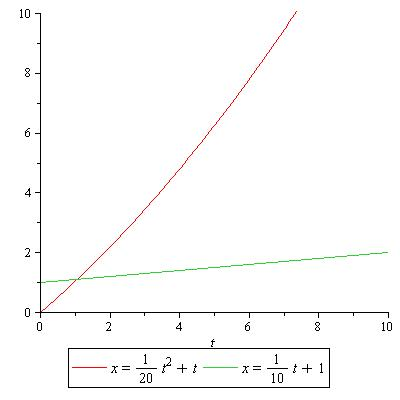
\includegraphics[width=0.5\columnwidth]{ChapterEcon/figures/smoothincretsjpeg}%
\caption{Basic `smooth increasing returns' function, showing total and marginal output.}%
\label{fig:backyardtoecons}%
\end{figure}
...
\begin{figure}%
\centering
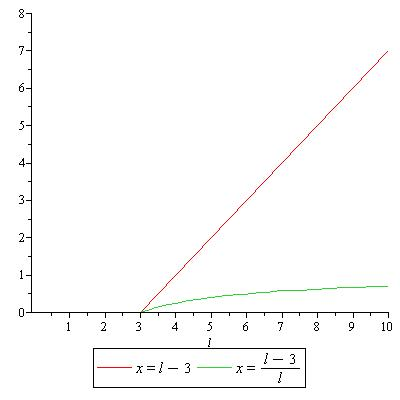
\includegraphics[width=0.5\columnwidth]{ChapterABM/figures/coremodelprodABMjpeg}%
\caption{Core model production function showing total output and average output per unit of labour}%
\label{fig:coremodelprodABMjpeg}%
\end{figure}
..
Peoples' utility in the models comes from raw good consumption: no price enters directly into their utility function, only good amounts a person can acquire. It is the job of the person to optimise their time to get the best mix of goods they can. In fact (as with the simple production function above) there are difficulties with using optimised utility functions that include price in an agent context: using `raw' good amounts is the best way of letting people find their optima. Again, this is explained in depth in section \ref{sec:twogoodsmodels}. 

%Cut out `space into utility and production', moved to framework.

==================
...
It is not unusual for a particular technology or current intellectual trend to find itself held up to reality; the same thing happened with both Newtonian physics and Darwinism. 
...
Epstein, isomorphism etc
p.24: 
``We noted earlier that markets can be seen as massively parallel spatially distributed computational devices with agents as processing nodes. To say that `the market clears' is to say that this device has completed a computation. Similarly, convergence to social norms, convergence to strategy distributions, or convergence to stable cultural or settlement patterns, are all social computations in this sense. Minsky's (1985) famous phrase was `the society of Mind.' What I'm interested in here is `the society \emph{as} Mind,' society as a computational device. (On that strain of functionalism which would be involved in literally asserting that a society could be a mind, see Sober 1996.)''
Goes on to note that in some cases `the isomorphism with societies is direct'. 
Occurs to me my alien world analogy comes out of this naturally: if Epstein and others are right about `synthetic empirical data', that's empirical data from a world very different to our own. Which makes them alien worlds – so we're going to have to be careful about any comparisons we make.
Ah: that does actually lead in to thinking about `the game', and asking, is the dynamic `the same thing?' in some sense. I guess I want to ask a different question, since ultimately it's not a testable statement – it can only be asserted. 
%`sufficient to generate' and all that: ``a good fit demonstrates that the target macrostructure - the \emph{explanandum} - ... is effectively attainable under repeated application of agent-interaction rules.'' [8]
%“The generativist manifesto” - !
%He's questioning `emergence' here. He has a good question: ``how ensembles achieve functionalities (or properties) their constituents lack''. Thinking of space: in a sense, they don't. They just produce more welfare. That said, an economy does have different properties to a person.
%``The agent-based computational model is a new tool for empirical research. It offers a natural environment for the study of connectionist phenomena in social science.'' [4]
%– but more strongly, that the micro-actions involved do not contain an intention that would lead to the macro outcome. (This is the same as the `invisible hand' argument: many selfish actions lead to the best of all possible worlds.) 
% Just to remind myself: I think the alien world argument is a reasonable one. Equation descriptions are alien worlds. Krugman's core model is. One of the big drawbacks I'm saying agent modelling has is: because it is possible to identify agents with real-world actors, it is easy to take the obvious step, and conclude that closer mappings are better. In a way, at least equation models suffer less from this tendency.
...

Cut the last line cos of `thesis 3', paraphrase: Hoover points out that, in contrast, defenders of the representative agent tend to think ``the only acceptable or useful macroeconomics is microfoundational.''
Ties to the Lucas critique to micro-economics - ``in economics, the only acceptable causal articulation must capture the intentional actions of economic agents.'' (p.332)
That ties to Koopmans on the different stages, Newton and gravity as an explanation.
...

\subsection{Heroic assumptions \label{sec:heroicassumpts}}
Heroic assumptions:
Ha – yes, like. The big question here, which I have written down somewhere. Tying to Feynman, to choosing your simplifications. Well, the argument is, it's not much good you giving me a mea culpa: yes, I know, the model has silly assumptions. You haven't then gone on to explain to me why or when that's OK. The idea of heroic assumptions tends to be used when someone suspects they're looking at a simplification that's gone too far. 
So, simplification can be useful for thinking about a problem, even if the model is `wrong'. 
There are always deeper complexities, so in fact everything is a simplification at some level. 
Blah!

%Economics, \gls{ge} and location theory are replete with `heroic assumptions'. The phrase itself has been in use for a great many years; one reviewer  of the English translation of Weber's `Theory of the Location of Industries' (\citealt{weber_theory_1909}) in 1930 warns, ``in approaching this book the reader must be prepared to meet a very abstract treatment and some very heroic assumptions'' (\citealt{fetter_review:_1930} p.233}). Much later, Brakman \emph{et al} note that the same type of heroism led to the success of the \gls{dxs} (\citealt{brakman_new_2009} p.93). The phrase appears to be quite common. From context, it seems that a heroic assumption is characterised by two things: being highly unrealistic, but opening up new avenues for analysis. As such, they have always been an easy target for critics, and \gls{abm} theorists have certainly taken aim at them. 

There is, however, a different problem with heroic assumptions: they are generally the consequence of analytic necessity forcing some simplification on the modeller. The resulting analytic models cannot easily deviate from the tracks thus laid down. (\gls{ge} writers (and Krugman especially) have, to their credit, been very self-aware in discussing these constraints and their implications.) What this means for any attempt to take ideas from \gls{ge} and apply them to \gls{abm} is very different types of constraint present themselves. Because of this, there is not always a clear way to `translate' one into the other. In fact, when working through model development, the ways in which one relates to the other can seem so unique, it is very hard to define quite where these differences come from.

The actual details of where in model development this manifested itself are written up in chapter \ref{chapter:models}. The main point to take from this for the rest of the chapter here, however, is just this: a knee-jerk reaction against simplification does not help analysis or the development of an \gls{abm} model. Different approaches have different limitations, and \gls{abm} itself most definitely has its share. So one goal of this chapter is to understand what they are.

%WUD 18	The realism-relevance argument. Same as GE arg: depending on what you want to analyse, you have to be selective about what you're willing to do damage to. As implied here, it's a judgement call.
%p.s. just remembered Blaug has a paper on this. Worth remembering the history of economic thought on this; no year zero necessary.

%\section{Bits from original introduction}

%But what of \gls{abm}? On the face of it, ABM is a perfect tool for the job. The analytic approach of GE is - as Krugman himself acknowledges - a `mathematical straightjacket' (\citealt{martin_new_1999}). The core model is bound to a particular approach to monopolistic competition built on a 1977 Dixit \& Stiglitz paper (\citealt{dixit_monopolistic_1977}). Its engine is the `constant \gls{eosub}' function. As \citeauthor{fujita_spatial_2001} note, it can sometimes seem like GE is all about ``games you can play with CES functions'' (\citealt{fujita_spatial_2001}, p.6). Unhindered by many of the restrictions that afflict analytics, is ABM not perfectly placed to explore locaton theory more freely? The fact is, however, this promised freedom has not led to great new theoretical vistas of success. Why not? One possibility is that precisely those things ABM claims to be good at are actually its weaknesses. Heterogeneity, diversity, many interactions - all of these can be abstracted away in analytics with no loss of strength - and perhaps, in fact, with a large gain in clarity. 

Kirman
"The market provides the mechanism which links and coordinates all the activities being pursued by individuals. Paradoxically, the sort of macroeconomic models which claim to give a picture of economic reality (albeit a simplified picture) have almost no activity which needs such coordination." [117]

``whatever the objective of the modeler, there is no plausible formal justification for the assumption that the aggregate of individuals, even maximizers, acts itself like an individual maximizer. Individual maximization does not engender collective rationality, nor does the fact that the collectivity exhibits a certain rationality necessarily imply that individuals act rationally. There is simply no direct relation between individual and collective behavior'' [118]

\begin{quote}
``then "the `representative' individual is being used to \emph{provide} the stability and the uniqueness of equilibria which are not \emph{guaranteed} by the underlying model.'' (ibid p.120)
\end{quote}


"I claim that economists have been forced into doing this by their insistence on `satisfactory' microfoundations." [119]

Oh - this is a very good point I hadn't really grasped before: "The uniqueness of equilibrium legitimizes the use of comparative statics to evaluate the effects of changes, particularly policy changes, on the economy." [119]

If no actual process exists to get back to the equilibrium (e.g. tatonnement) - then "the `representative' individual is being used to \emph{provide} the stability and the uniqueness of equilibria which are not \emph{guaranteed} by the underlying model." [120]

There's a point here that overlaps with Kirman's: space costs mean its impossible that all actors will be affected in the same way by changes.

...

Gosh: "It should be clear by now that the assumption of a representative individual is far from innocent; it is the fiction by which macroeconomists can justify equilibrium analysis and provide pseudo-microfoundations." (p.125)

Makes a great point: many problems could in fact be made considerably more complex using a representative agent, "when aggregating over several heterogeneous and myopic individuals who analyze their income processes in a much simpler but still consistent way may produce a similar result." (p.126)

"... complicated dynamic behavior may arise from aggregation over heterogeneous agents with simple behavior." (p.127)

"Rather than proposing ever more complicated dynamic optimization schemes for representative agents, it makes sense to explore the patterns that may develop from aggregation over heterogeneous individuals, who make simpler but still coherent calculations." (p.127)

Increasing heterogeneity can be stabilising. (p.129)

"This result will come as no surprise to those familiar with Cournot's observation that erratic individual demand behavior may give very smooth aggregate demand behavior, if individuals are different enough." (p.129)

Reminded of farmers deciding when to sell produce: aggregate result is smoothed prices over the season.

His example is better: consumers with hetero, non-convex preferences. Demand may "jump from one bundle to another at certain prices", but if hetero, that can still lead to smooth, comparable changes. If it were a rep agent, that would not be the case.

Ah: that's actually really useful, because it shows a qualitative difference between micro and macro. And actually it means a rep agent might work, just as long as you weren't claiming it represented actual micro behaviour.

"The open question now is to what extent can dispersion of characteristics help us to regain structure at the aggregate level." (p.131)


Large chunk of notes from printouts

E.g Eos: (MM2 43) Firms should be able to exploit EoS, but how should that happen? Cf MM1 42 backyard.
MM1 66: firms with higher inputs of labour should have an advantage - they should be able to find a better price than others, if they're ahead; they should have able to get a monopoly.

The point there: geneq is meant to do this; account for all those dependencies. Cf. Fowler.

WUD 4	``Although a full description of this alternative is beyond the scope of this article, it appears that the choice of asynchronous rather than synchronous decision-making is not a key point in understanding the differences between the agent-based and analytic models.'' (Fowler 274)
I disagree! Big, complex issue. Order and randomness large effect on outcomes. Maybe not so with Fowler's very small number of agents.

WUD 22	Auctions vs on-line adjustment versus simultaneous eqs. Actors' decisions spread over time = normal.

FDA 16: Trapped in loops of dependency! Where to work, what to buy, who to hire, where to locate? All affect each other. 

Update: I should just note quite how much I struggled with this problem initially. The answers wer far, far from obvious. I have a solution that runs, but a) many more must exist and b) it may run, but does it really work?

Quote from Fowler: ``the amount a firm can offer in wages is dependent on the amount it can produce and price it receives for its goods. These quantities are affected, in turn, by consumer's wages, which depend on which firm employs them (and whether or not they have found employment at all.)'' (p.277)
There's intrinsically a limit on what agents can do to solve these problems. There's game theory: trying to optimise under uncertainty. But it's not a problem of lack of information: it's a problem of incalculability. 
This may mean, also, that - say - the resulting number of firms is due to a random number failing; no way to predict who, but the incalculability of the problem means that only some will make the right guesses. Cf. Baumol quote on what firms should do to optimise.
Also noted here that the landscape itself is a form of memory.

From Oeffner:
Incalculability: p.25. He talks about it in different terms, but it's the same issue: a difference between 'risk' and 'true uncertainty' stemming from the fact that you don't know what other agents are going to do. Ties to data, meaning
'Endogenous uncertainty': Pesaran 1987. On p.27. That's exactly the problem with two firms trying to find a good location. 


FDA 17	Agents deciding when to sell. Fream: farmers releasing goods in a way that smooths prices. Cf. Kirman's argument about the representative agent, and disaggregated models explaining this kind of smoothing.
The point there isn't so much that you can affect demand - you can, but the effect is small - but that you want to adjust your timing to fit with the macro-effect of supply on demand. You can't really affect prices, but you know prices are going to change in a certain way over time. So, you're a price-taker in the short-term, but there's a longer-term strategy that means you have some wiggle-room - so are actually not a price-taker - and the long-term result is a smoothing of prices. Again, Kirman.

WUD 1	Fowler: ``it is impossible for firms to make decisions about production levels without knowing exactly what every other firm will do and where labour will be available.'' (p.265)
But they don't need to: blind groping. 

WUD 1	Common goal of 'perfect information' vs 'groping' agents: optimisation. Question: how important, if at all, is the 'realism' of the agents? Mine aren't at all. One arg: objective existence of optima; nature of agents doesn't matter; disaggregation is the thing. Fowler: : ``Agent-based modelling works by disaggregating the modelling environment to the extent that each firm and agent is represented as acting individually.'' [265]

==
WUD 2	Determinacy, uniqueness, stability. Necessary for equation-based results? ABM: randomness = come up with probabilistic answers. 
WUD 3: Useful quote, Fowler: ``The economy as it has been represented in geography is typically far too chaotic to be considered at rest or to be operating at some market-clearing point where all labour is employed, all production is consumed and utility is maximized (Plummer et al., 1999).'' (p.271-2) No-one claims that the real economy will reach a rest point, only that the models help us understand the equilibria it moves towards. Think ball on rubber sheet in high wind.
Plus, if completely blind agents can find their way "on-line" to optima, that chaos doesn't present a problem. May be too chaotic to be at rest, but not so chaotic that optima can't emerge through blind luck (and not evolution, unless one considers the landscape as an evolutionary memory. If so, it's Lamarkian!)
There must be a trade-off between how much the world is changing and how much blind groping can achieve, and it must relate in some way to this point about equilibria and change. God knows how though.  
Plus, do agents only capable of telling better from worse count as rational?
WUD5: If a model can grope it's way to optima, with agents' only ability being that they can compare 'before' to 'now', what does that say about the economics? I think this: the equation approach is still entirely valid, but perhaps it's not describing micro-motives. Perhaps instead it's illustrating where the optima are and nothing more. The appeal to utility as a mechanism is false: no action is taken to reach that optima.
One might argue against that: if it can be shown that agents can indeed reach those optima through groping (cf. Walras) then we can assume the mechanism and continue to use analytic optimisation. I'd reply: you have to show that the mechanism does, in fact, work. 
update: which is Epstein's point...
==

MM1 8	Granular, on-line, no market clearing to be done. The many many uses of blind groping.
MM1 15	Supply and demand: stochastic, iterative, not 'clearing'.


===
MM1 18-	Write-up of optimisation and GA. Most useful algorithms assume that there will be some correlation between the quality of 'neighbouring' candidate solutions - those close in the space. Genetic algorithms assume that high-quality 'parent' candidate solutions from different regions in the space can be combined via crossover to, on occasion, produce high-quality 'offspring' candidate solutions." [Mitchell GA p.7]
"What is maximising on-line performance good for? Holland's view is clear: the rough maximisation of on-line performance is what goes on in adaptive systems of all kinds, and in some sense this is how 'adaptation' is defined." [124]
On-line performance: stealing that idea. That was previously "live groping!"
Satisficing.
Worth-noting: GAs combined with hill-climbing algorithms often found to work better than GAs alone. [124] Would seem very likely to be the case for my agents. "GAs seem to be good at quickly finding promising regions of the search space, and hill climbers are often good at zeroing in on optimal individuals in those regions." [124]
Cf. MM2 73: "crawling around in utility space, possibly attempting to swim up a too-turbulent stream and not finding their way..."
===
MM1 42	Cf. split decisions of beanworld; separate auctions for work time and bean buying.
MM1 42	Contrast: backyard model, where actors are able to immediately know whether a particular decision will be more productive for them; indeed, the decision can be taken to be the production, it's so simple. Not so here: the EoS necessary to ultimately lower the cost of production can't happen without a number of people working for a firm; yet, that won't happen below a certain critical theshold, or possibly can't happen at all, given the way I've coded it.

MM2 65	Discussion: the more blindly agents can find optima, the more one can say the objectively exist? Cf. fact the agents make the world they're optimising in, so it can't really be objective can it?

MM2 73	Details of person action choice 2, random groping. So, they might try wage - thus producing stock, thus breaking out of catch 22.

MM1 15	The trick: actors deciding "as if" others are still contributing their time. Need to write up, perhaps compare to simple game theory example

===

MM1 41	Stock running out for some firms shouldn't mean they can't hire - if they have the money. Cf 2 optimisation choices and problems.
MM1 42	Does the stock-crash end-of-model problem say anything interesting about the real world? Is it anything like a co-ordination problem? I.e. people want work, firms want to sell goods, catch 22?
Breaking out: letting work happen before stock levels are known. Is this just a practical modelling solution or something about the real world?
MM1 42	Cf. split decisions of beanworld; separate auctions for work time and bean buying.
MM1 42	Contrast: backyard model, where actors are able to immediately know whether a particular decision will be more productive for them; indeed, the decision can be taken to be the production, it's so simple. Not so here: the EoS necessary to ultimately lower the cost of production can't happen without a number of people working for a firm; yet, that won't happen below a certain critical theshold, or possibly can't happen at all, given the way I've coded it.

More cuttinz
Ideas from the history of physics can be particularly fruitful for thinking through economic and agent-based problems, if only to illustrate when physical and social modelling differ incommensurably.
%I'm thinking here of using gravity as a good example of where the explanans/explanandum distinction could go further, but that at one level it does all you need it to.
The structure of \gls{ge} and \gls{abm} are entirely different. They are built on different foundations, and consequently have developed separate philosophies for model development. This may seem an obvious statement, but the consequences are not always so clear. The central lesson is that a direct translation from one approach to the other is not possible. Section \ref{sec:fowler} discusses Fowler's attempt at recreating the \gls{coremodel} in agent form. Fowler does an excellent job of demonstrating the point just made: it doesn't make sense to directly translate the neoclassical core model into the computational form of an agent model.
...
One might respond, that is all very well for physics, but Friedman erred in applying these standards to the social sciences. Perhaps so, but that does not nullify Friedman's point.
...

But is this sort of counterfactual (``what if...'') of any real value? If it done carefully, perhaps so. For the present thesis, two points are worth noting. Firstly, Hayek holds a special place in the hearts of some agent modellers: this draws attention to \gls{abm}'s tunnel-vision focus on complexity. Secondly, there's a question hidden in this line of thinking - precisely how much does the knowledge and technology of a particular era carve the channels that theory-making must take?
This is a mistake, because it means too much is lost; there is no simple shortcut that can offer a way to dismiss an entire body of theory in this way. The job of this thesis is to disassemble some of the key components that make up \gls{ge} to see how they work. Only then can a direct comparison with an agent-approach have any chance of succeeding.
...
The tight fit, the close isomorphism, between reality and physical models means we trust those models to predict, we trust them with our lives. But it still hides the basic truth that physical models are still only a description, a way of representing reality. 
...
As discussed in the introduction\cmt{``As discussed in the introduction'' - not yet}, any comparison between a \gls{ge} and \gls{abm} approach to location theory needs to explain what it aims to achieve from doing so. One stated aim, for example, is to find out what \gls{abm} is actually good at. Does it have any strengths that make it able to analyse problems beyond the reach of an analytic approach? In short, is \gls{abm} better at some things than \gls{ge}, and vice versa?

But this begs the question: what does `better' look like? The job of this section is to find some candidate answers to that question.
...
Clearly, it is not possible to ask \gls{ge} and \gls{abm} to churn out `substantive propositions' and find out which has the most - but this does offer a tool for comparison. What propositions can each give? Can they both say something about propositions the other makes, or are they producing very different ones?
...
\section{The doughnut of empirical correctness \label{doughnut}}

``The doughnut of empirical correctness in a theory constitutes its worth, while its hole of untruth constitutes its weakness.'' Samuelson in Blaug 1980 p.97.

\section{Using the maths in the models: what does it mean? \label{sec:mathsinmodels}}
==========
%%%%%%%%%%%%%%%%%%%%%%%%%%%%%%%%%%%
% CUTTINZ
%%%%%%%%%%%%%%%%%%%%%%%%%%%%%%%%%%%
%The result was that ``workers locate without regard to labour demand in a particular location

%One element in particular that he focuses on is the equilibrium number of firms - a key feature of of the Dixit-Stiglitz \gls{monocomp} approach. As discussed in section \ref{sec:marketstructure}, firms are derived from consumer demand. They have no independent, decision-making existence as such: ``the number of firms is simply a function of the labour required to produce a fixed optimal quantity of goods.'' (p.270) Given that agent modelling demands that firms exist as separate entities, this presents an immediate challenge for Fowler's attempted translation to an agent model. 
%``... the model assumes that the number of firms in a city is defined based on the amount of labour available in that city and the amount of labour necessary to produce the optimal amount of a good.'' (p.271)

%The direction taken by this project goes the other way: start with agents and work towards the concepts used in \gls{ge}.
%... This thesis comes at the problem from the opposite direction, in two respects. 

%He suggests this finding should lead to caution about making any policy claims based on the core model. I rather think it should instead lead to saying: agent models are different from their analytic counterparts, and those differences have to be respected. You cannot build a model of consumers and firms  - with explicit firms - without specifying how they interact. (You could perhaps model agent consumers and deduce firm numbers somehow, without explicitly creating firms as agents...) If the analytic argument about that interaction does not translate, then one that fits with an agent approach must be constructed.

%One reasonable alternative to a set of equilibrium solutions is a model that incorporates bounded rationality and the possibility of error. In this type of model, 
%Later: ``To create such a model, firms would have to have some mechanism with which they could predict an appropriate production level for themselves and estimate the levels chosen by their competition in an environment where sufficient labour supply is not guaranteed. 
%I should try and end up with a list of aspects of interest. So, these are things that ABM particularly draws attention to. To include:
%- how demand should work. Fowler goes for objective budget.
%- mechanisms for: linking production to labour; wages to employment. (So says Fowler.)
%- equilibrium level of firms. The connection between demand andntry/exit

%Hey! The seques nicely into a discussion on equilibrium, doesn't it? Aaawesome-ee-doo-dah!

%\begin{quote}``The logical step to improve the functionality of this model is to develop equations that account for the rationing of wages and production, based on worker employment (for wages) and availability (for production)... the model must be reformulated from its most basic assumptions before such rationing can be incorporated to move forward in this highly desirable direction.'' (\citealt{fowler_taking_2007} p.277)\end{quote}

%This is, of course, exactly the kind of argument Hayek was attempting to counter: success in providing a model rationing system would end up saying nothing about the fundamental problem of how disaggregated actors can coordinate production. There are benefits, however, to the `subjective' approach of testing possible goods bundles against utility, parallel to the benefits of blind search: no prior knowledge of the state of the market is required. Actors can act based on the informatin presented to them.

%Fowler quotes Amin and Thrift calling for a ``move away from the long shadow of economics'' \fixref{(Amin and Thrift 2000)}. Again, the direction of this thesis is actually more towards some aspects of traditional economics. 
...
%nice summary of the f-twist here: http://motls.blogspot.com/2009/02/milton-friedmans-f-twist.html
%This will need writing up much better and more carefully, if I do end up using it. I think I probably should.
Friedman's chief point here is one that has caused a great deal of consternation, and offered an easy line of attack for theorists unhappy with the simplifying assumptions of economics. Called the `F-twist' by Samuelson (see \citealt{blaug_methodology_1992} pp.91 for an overview), the caricature version says: `model assumptions don't matter, and don't have to be realistic. The only thing that matters is predictive power.' This is an unfair interpretation. Einstein, for example, made the same point as regards physics:

\begin{quote}
``Physics constitute a logical system of thought which is in a state of evolution, whose basis cannot be distilled, as it were, from experience by an inductive method, but can only be arrived at by free invention. The justification (truth content) of the system rests in the verification of the derived propositions by sense experiences. The skeptic will say: `it may well be true that this system of equations is reasonable from a logical standpoint. But it does not prove that it corresponds to nature'. You are right, dear skeptic. Experience alone can decide on truth.'' (A. Einstein, Ideas and Opinions, New York, 1960, pp. 322 and 355 (quoted by Kornai, op. cit., pp. 9-10), quoted in \citealt{kaldor_irrelevance_1972} p.1239.)
\end{quote}

However, there are very separate challenges involved for what this means in physics and in economics. Whether or not the universe `really is' as relativity describes has quite different consequences to whether people `really are' rational, constrained optimisers. 
...
J Stephen Lansing and James Kremer's model of Balinese rice management is a good example of an ontological prediction from a very simple simulation \cite{lansing_priests_2007}. Attempts to apply Green Revolution-style growing techniques to Bali were actually damaging the existing rice-growing system. Lansing had tried to tell the authorities about the role that the Balinese water temples played in finding an optimal trade-off between fallow and growing that maximised yield and minimised pests, to no avail. However, when Kremer helped Lansing model the system, and the key dynamic became easy to explain, they had more success. This was an ontological claim: a simple model that demonstrates a mechanism that manages rice production, in a way that appears to capture the salient features of the real-world system. 

This is, perhaps, what Epstein claims is happening in `generative' social science.\cmt{`This is, perhaps, what Epstein claims is happening in `generative' social science.' This is its first mention.} If so, Epstein is wrong to claim that `growing it' can count as `explaining it'.  Generating a model phenomenon offers only a hypothesis - one of Friedman's `substantive propositions'. The tautology of the model still needs to be theoretically tied to the real world.  Does this mean models are \emph{only} analytic engines that output hypthoses, not explanatory tools? 
...
in the process of actually attempting to make a model of spatial economic activity, and precisely for the reasons Hoover cites: many ways exist to make models appear more `realistic' through carefully matching code to real world structures, but this approach offers little in the way of analytic insight.
...
Abstract models allow for concentrating on the relationships between variables in the model: to come to a full understanding of how they work, separate from calibrating against real-world data, which can actually cloud the ability to see what is going on, if data is not used in the correct way.
\cmt{bring in di paolo}

There is no point in simply adding data to a model. The problem here is that it can always be done: data can be added in a myriad of ways. But there are only a very few ways for it to be used appropriately, and the tendency to mistake `includes data' for `is therefore more realistic' is strong.
%I wonder if the Bali model would have been accepted without actual rainfall data? The abstract picture: less appealling to people who want to see simulacra of reality. 

Of course, ultimately, reality is the arbiter of all models. The purpose of this chapter, however, is to ask exactly how this comparison to reality should inform the model builder, and what role the `thought experiment' model has.

My conclusion's going to be something like: the commonly-held view of model `validation' goes back to statistical tests against data: `fitting' is commonly held to be a suitable goal. However, the reality of model-building, interpretation and use in the social sciences is much less clear-cut. The role of the modellers' interpretation plays a much larger role, as does the form of `praxis' involved in particular disciplines. Missing the fact of this praxis may be responsible for why critics often mistake economists' models for their actual understanding of the world, rather than tools that aid that understanding.
\cmt{`tools that aid understanding': repeated that line here. Make sure to delete it from one of the two places it currently resides. Plus: whole para is dodgy-lookin'!}
...
. But that is precisely the point: models should have a `functional mapping'. This does not require models to be as realistic as possible, or that the code structure imposed by \gls{oop} is better if closely mapped to reality. What does a functional mapping look like?
...

`Construct a language that will yield as many substantive propositions as possible.' 

Milton Friedman offers one answer. As Leeson notes, Friedman argues that theories are tautologous forms of language - they cannot directly provide their own criteria for success: ``the relevant question to be asked is usefulness and not rightness or wrongness'' (Friedman 1953 p.7 quoted in Leeson.) They must function as `engines of analysis', producing propositions that \emph{can} be held up to the world. This leads Friedman to say that one should - 

\begin{quote}
``Construct a language that will yield as many substantive propositions as possible.'' (Friedman 1962 p.8)
\end{quote}
...
%not sure where I'm going with this, so let's try a different tack...
The aim here isn't to develop a historiography of economic theory in any great depth; the point is that, when comparing \gls{ge} and \gls{abm} approaches, the foundation stones on which they are built can help a great deal in making that comparison transparent. As regards \gls{ge}, a theme that runs through explanations of chosen methods is compromise - the analytical gains made by finding mathematically tractable ways of describing a problem.
..
BITS FOR THIS SECTION
%==============================
WUD 4	What does the computational approach impose? Asynchronicity, possibly. Hence my trick to get round strategy. 
WUD 24: how do physics methods and computing methods define the nature of the location problem differently; what does this mean for 'translating' one to the other? Do the different foundations make them mutually exclusive?
...
As Blaug points out \fixref{blaug on Walras} when discussing Walras, one might argue there is a fine line between using those tools to help gain insights into how the economic world works, and mistaking those tools for reality. 
...
%I think the argument that Blaug has, looking at e.g. Walras, is that somewhere there's a line crossed between using those tools to help gain insights into how the economic world works, and mistaking the tools for reality. This is perhaps the point that Friedman is making. 
...

The \emph{kind} of propositions any particular 'engine of analysis' can produce matters too. \gls{ge} comes from an international trade perspective - it wants to be able to say something about why places trade, and why they can end up with such disparate wealth. A key proposition it gives is this: in the model, it is possible for regions to diverge due to endogenous forces; there is no need for there to be any difference in initial factor endowment. \cmt{mentioning GE's `substantive propositions' here - worth cross-reffing with wherever I end up writing them up in detail.} Notice that sentence started with `in the model'; the next question must be, `is it possible to find some element of reality that can offer support to this proposition, or falsify it?'
\cmt{A point here: questions asked are very diff. cf. Epstein, can you grow it? Discussed in Epstein section.}

\cmt{What I want to argue somewhere: current thought on transition and energy is offering a whole bag of propositions. What I want theory to do is to give us substantive propositions that confirm or deny the statements made, or offer interesting new ones that nevertheless might shed light on those issues. GE deals with a very different proposition 'base'. It's all about trying to explain the core-periphery pattern as 'an endogenous process...' Is it really any good at answering the kind of questions I'm interested in?}

Cf. allotment example, in general examination of utility
...
\gls{ge}'s insistence on the need for micro-foundations reflects a perfectly understandable desire to explain why spatial systems produce the outcomes they do. But might it be possible that \gls{ge} has things backwards?
%notice the crossover here with 'operational' vs 'scientific' models trying to work out how the world works. That book on planning, good for this. Should go in write-up on 'thought experiments' etc.
...
This is a rare commonality, however. GE ``aims to explain the formation of various forms of economic agglomeration in geographical space using a general equilibrium framework'' (\citealt{fujita_frontiers_2005}, p.377). This framework is the main fracture line between GE and ABM. GE is impossible without it; ABM not only manages outside of equilibrium, many argue that, precisely because it can do this, it can more closely mirror reality. (E.g. Tesfatsion  - see chapter~\ref{chapter:ABM}.)  
..

%Provides reason for talking about GE, cf. 2 agents with basic utility
\gls{ge} theorists argue that the modelling approach's strength is built on solid micro-foundations. [quote from krugman 96 here?] What happens at the level of the whole economy (the `macro' level) flow from how agents' behaviour and interaction are theorised (the `micro' level). If \gls{ge} succeeds in this, there would appear to be little point in attempting an agent-based approach: this would just add complexity with no further insight, and possibly even a loss of clarity. 
...
Despite seemingly approving of the need for a `Kepler stage', Koopman politely attacks the empirical void in Burns and Mitchells' analysis of business cycles; they aim for:

\begin{quote}
``... faithful observation and summarizing of the cyclical characteristics of a large number of economic series. The toolkit of the theoretical economist is deliberately spurned. Not a single demand or supply schedule or other equation expressing the behavior of men or the technical laws of production is employed explicitly in the book, and the cases of implicit use are few and far between.'' (ibid p.163)
\end{quote}
Can similar reasons be found in earlier and more recent economic analyses? Can the answer help shed any light on what kind of model choices should be made?
..
Neoclassical economics and \gls{abm} share a common thread: the use of abstract models in the development of ideas. However, defences of the use of such models greatly differ between the two. As discussed above, many leading lights in the \gls{abm} field have argued that in some sense, abstract agent models can be directly compared to reality. 
..



%There is a classic Hayek quote here: ``the problem is thus in no way solved if we can show that all the facts, if they were known to a single mind (as we hypothetically assume them to be given to the observing economist), would uniquely determine the solution; instead 
, he criticises Schumpeter for using ``objectively given quantities of commodities impinging directly upon each other, almost, it would seem, without any intervention of human minds''. Hayek quotes Schumpeter as arguing that -

\begin{quote}
``... the possibility of a rational calculation in the absence of markets for the factors of production follows for the theorist `from the elementary proposition that 
\end{quote}

\cmt{this crosses over with args about monocomp, e.g. in Fowler section.}
...
the important part for the argument being made is that Hayek believes Schumpeter to be ``disregard[ing] everything that is important and significant in the real world'' (ibid p.530). 
..
This is examined in more depth below\cmt{`people are not like that': examined where? Now, I think?}, but it is useful to quickly explain the thesis' position on this: people are not utility-maximising automatons, but utility theory \emph{is} a useful way to analyse how people react to changes in costs. There is no need to make any sophisticated case for the psychological basis of utility; it can still be used as a modelling tool. Neither does this mean more sophisticated models of behaviour are unimportant: utility is merely a simple, effective way of gaining insights into the impact of cost changes. There are some pitfalls to be avoided when interpreting utility-based agents; these are discussed below.
..

this focus on agents as things you let loose and then observe has encouraged a view of them as empirical worlds in silico.
Tie to epstein;
More on – 

These two trends in agent modelling - a push for more and more `realism' in the structure of agents themselves, coupled with a narrative about complexity - have perhaps distracted from the simpler ideas that \gls{abm} has made possible. The next section starts to deal with this point in more depth by examining how models should map to reality.

%For this thesis, the important ideas are those that offer a way out of strictures imposed by analytic approaches to spatial economics - namely asynchronous decision-making and an ongoing, non-clearing market mechanism. 
%\cmt{async, non-clearing: where have these things been discussed?}
..
Not wanting to get too far into arguments about causality, it is nevertheless interesting that similar arguments occurred as gas theory was being developed. 

``The establishment of Boyle's Law has considerable philosophical importance in the history of science, because it was the first numerical law which illustrated the functional dependence of two variable magnitudes. Such laws provide important illustrations of the failure of the idea of causation in the Aristotelian sense - since any change in volume is strictly concurrent with the change in pressure, there being no justification in assuming that the relationship is asymmetrical or sequential'' (\citealt{webster_discovery_1965} p.494).
..
Society self-organises (and evolves) through `connectedness of fragments of knowledge; connectedness requires that over all the individuals there is complete knowledge of [the system] though none possesses it individually.” (Desai p.42)  
Hayek does seem a little over-enthusiastic in his defence of the sovereignty of tacit knowledge that prices reflect. His theorising `asserts what it was meant to demonstrate'. (Desai p.46)  
…
%This can lead to `fundamental misspecification' arg... cf. Oakeshott and Baumol. This is exactly opposite to Baumol's physics/engineers comparison - ``A complete mastery of the principles may exist alongside a complete inability to pursue the activity to which they refer, for the pursuit of the activity does not consist in the application of these principles; and even if it did, the knowledge of how to apply them is not given in the knowledge of them'' (\citealt{oakeshott_rationalism_1962} p.101 quoted in \citealt{scott_seeing_1998} p.316).
..
The second, related condition imposed by explicit space is that actors naturally form networks. Take the most basic example from section \ref{sec:spacenutility}, which outlined the simple rule \eqref{eq:circlerule} defining the set of actors' neighbours simply as `others within a given radius'. Actors face overlapping groups of potential trading partners: as well as making it impossible to assume that all prices can be simultaneously adjusted, as just discussed, this can be used to define a network.

This form of spatial graph has been studied in both discrete and continuous forms, and in an agent context.
\cmt{Think I'll wait on these refs to see what I write next...}

The theoretical existence of these network properties is not always relevant to model outcome. In the backyard model in section \ref{sec:backyard}, for example, while actors have the option each turn of deciding on a collaborator, one central site quickly becomes locked in. As soon as this happens, any potential network effect disappears. In more complex models, however, the network structure becomes more important. The density of actor networks within possible travel radii is the foundation for cost signals. In this context, agglomeration and space cost changes will impact on these network effects by moving the model towards stronger synchronised signalling. 

%Networks connect to diffusion, of course: so, price signals, demand signals may diffuse. 1D model perhaps best for trying to trace how that works.

%

%So I model granular agents; I've written about that, possibly in zotero notes for the last comp handbook chapter.
..
Utility cuttinz
A thought: as mentioned below – utility, or more specifically `how people react to cost changes' may do particularly well for how people react to space cost changes. If something like that does work at the individual level, agent modelling might show interesting results. Alternatively, utility may turn out to be better as an aggregate description, with no qualititative connection to the micro level at all. There is then a different job showing how the levels connect, but it's some way beyond just saying `microfoundations' and using a representative agent model. 
Utility should be thought of not in psychological terms, but just as a descriptive, neutral shorthand for `how people react to cost changes'. This does not negate the validity of investigating the details of how people come to make the choices they do, but it is a different level of analysis. 
..
%``Clearly, by relating the notion of rationality in economics in this way to the pursuance of self-interest, one has "emptied' the notion of rationality of all substance. The merit of the Chicago School is that they have made this point so clear. Pushing the logic of economics to its limits, and following its line of argument consistently into every conceivable comer of social events, they have demonstrated that the rationality postulate is necessarily constrained to be essentially contentless in economics.'' [269]
%Rationality in economics means that an individual agent chooses (one of) the most advantageous options, given his preferences, in his perceived opportunity set.'.' [268]
%``the need for abstraction from psychological issues concerning the perception of opportunities'' [42]
%``the notion of rationality was practically non-existent in classical and neoclassical economic discourses'' (\citealt{vriend_rational_1996} p.265-6). 
%True enough, but I can imagine some situations – particularly where the process is `online' in the Holland sense – that the way the choice set was arrived at would matter. 
%This is the main point for me: ``it might be that agents do sometimes display irrational behavior, that they do act against their own %perceived self-interest, that preferences themselves could be "irrational', or that there might be mental states that lead to a perceived set of opportunities that is "irrational'. Economic theory does not exclude that such phenomena do occur, but it abstracts from them. Assumptions of a theory are by definition abstractions from reality. 
%To the the extent that the framework is useful for analysing problems, making those allowances is a useful thing to do. The flipside of this argument is, as Vriend notes, a ``need for abstraction from psychological issues concerning the perception of opportunities'' (\citealt{hillebrand_artificial_1994} p.42). 
%that ``economists are definitely not in a position to contribute to an explanation of how a set of given physical stimuli, including both the agent's objective environment and his own brain status and activity, leads to a set of perceived opportunities''  (ibid p.280).
%Friedman on Walras: is attacking cardinal utility, mefinks. p.901. Walras working with something that can't actually be measured or compared. Probably worth mentioning in my section on utility.
%So yes: worth mentioning, really, that there's no way of escaping my actors having cardinal utility. Does not require any direct comparisons between them, but does mean we know exactly how much of anything they will buy. Not sure how different that is to the rep agent approach.
%Some things I need to cover:
%utility as tautology / hedonistic / actual internal description of psychological state. Problem of information, uncertainty. The point about realism.
..
%One of the subjects of the previous argument has been to ask whether it is justified to use agents with simple utility functions. This section looks specifically at arguments about utility itself. The case made here is as follows: In the model framework developed for this thesis (described in detail in chapter \ref{chapter:modelfw}), agents use a set of `standard' utility functions. The functions themselves have been covered in the previous chapter. Many agent-based critiques of economics argue that the utility-maximising approach is an unrealistic strait-jacket
%--
As regards this thesis, the crucial point is that no argument need be made about the underlying mechanism or the rationality of those making a choice between walking or driving to work. There is, of course, value in attempting to understand what underpins those choices, but equally there is value in accepting and applying the finding. The underlying causes may be complex, but this does nothing to lessen the importance of the result itself.
Space adds something different to the question of how people react to costs. There are a myriad of reasons why a straight cost might be more complex than simple utility functions can deal with. Tastes are particularly problematic. Consider Blaug's worry about `pecuniary canons of taste', where ``once consumers have developed the habit of judging quality by price, every change in price affects their taste'' (\citealt{blaug_economic_1997} p.338). So, for instance, reducing the price of your whisky brand may not lead to higher volume sales, since consumers interpret the lower price as a drop in quality. 
..
Ah OK: if only ordinal, derivatives can have no meaning beyond "positive" or "negative." [313] 1st der is index of marginal utility; the second an indication of DMU (or otherwise.)
..
Connect this to the point about realistic assumptions... 
.. 

Marshall has a go but "succeeding editions of Marshall's principles were marked by increasing caution and reticence as the work of Edgeworth, Fisher and Pareto began to undermine the earlier notions of measurability, addivity and comparability." [312]
The measurability of utility
..
Notes: indifference curves are an ordinal utility tool. [328] "The notion of 'indifference' itself is not subject to direct measurement." [329] Which means, given what we've just seen, DMU is impossible: "once the idea of cardinal measurement is dropped, the very notion of marginal utility as a uniquely determinable quantity loses all meaning. A diminishing marginal rate of substitution is not equivalent to diminishing marginal utility." [332]
Which is curious, because: it means repagent stuff works, but it's automatically going to make individual agent action problematic.
%``utility maximisation merely packages the prediction'' ibid
``Much of this opposition was based on a confusion between the two meanings given to the word `utility'. In the theory of consumer behaviour, utility is a quantity that is useful to regard an individual as maximising in the interpretation and prediction of behaviour. A utility function is nothing more than a way of describing an individual's preferences between various real and hypothetical alternatives. Such a function 
Re. demand theory: "it is perfectly true that it cannot get along without the assumption of stable tastes." [338]
Note: space perhaps makes utility a more stable proposition. Reacting to distance costs is more likely stable than to differences in good price...? 
So, notes objections to ``making utility the `explanation' of consumer behaviour'' [337]; that it "rests on bad or at least questionable psychology" and that also economics doesn't need those psychological explanations.
The problem is simply enough stated: if any outcome can be described as rational, then the theory is completely unfalsifiable. However, if rationality is not the goal, but instead a given reaction to cost changes... 
But it depends on what you're falsifying, and what you're able to falsify with the theory. Any description of gravity that we have isn't really in a position to falsify the graviton theory. It'd need some deeper level of data to uncover what's going on. 
...
Appears to put utility beyond any possibility of theoretical testing. 
...
But is that proposition true? The risk is this: whatever outcome actually exists in the world, the theorist \emph{starts} from the assumption that it must be the product of rational actors. The job of the model is then to conform to the world. This is, of course, tautologous: rational decisions lead to the outcomes seen in reality, and reality confirms that, indeed, rational decisions are the cause. No analytic insight results; indeed, it seems to actually nullify the point of making the model in the first place, and imposes a false 'model' on a reality that may well be far more involved. What role might social convention play, for example?

This suggests that, whatever role 'substantive propositions' from 'model engines' might play, it is not entirely straightforward. \cmt{I think I'm heading back towards the 'dialogue between model and world' stuff here. Though it's also that the model might predict well. And whether utility is a good way of getting how human system choices might work. Cf. example of pool player modelling. Where did I read that example?}
... 
%What are Firms' goals? Their over-arching aim is simple enough to state: maximise net revenue, which is gross revenue minus costs. If a Firm can stay afloat doing this, they can survive. This simple aim quickly becomes complicated when considering all the options then facing a model of Firm action. 
%Section x explained that, in the \gls{coremodel}, firms have a production function that gives them \gls{increts} from labour input. It was also noted that those \gls{increts} are analysed away: changes in welfare through production come about solely through changes in the equilibrium number of firms, and thus the total number of varieties consumed. 
%But Leijonhufvud's point applies here too: analytic approaches skip to the end of the process of production. They describe optima, and build that description on an explanation lacking specific actions to get there. Whether or not this approach is justified (a point discussed more below)\cmt{pointer} is beside the point when it comes to building an agent model of production: \gls{abm} applies its own restrictions here, forcing the modeller to work with specific agents, and specifying what actions they must take in order to manage production. (x-ref Fowler discussion.) As just mentioned, firms enter and exit the market also. An agent approach must decide how to address this, even if to explicitly avoid it. \cmt{“Whether that approach is justified... ” Wasn't that discussed in `levels'?}
%Contrast to what agent firms need to do; data, meaning...
%Plus, randomness, sequence, luck may also eliminate a certain number. 
%Cf. nature of optimisation; function standing in for process of groping, etc.
The success of \gls{ge}, then, is precisely because it finds a way for actors to avoid having to use strategy in decision-making. But as with all \gls{ge} work, this is done with some consciousness of the damage to reality it entails and an argument about why it is still valid. One of those arguments is tractability. In theory, \gls{abm} is not restricted by that need for analytic tractability - but this may be a curse in itself, if this leads one to believe that all the elements of reality that Tesfatsion lists must be incorporated.
Which maps back to the mapping argument, as well as `levels', which is coming up.
..
Two areas of \gls{abm} should, in theory, be relevant:

\begin{enumerate}
	\item Spatial agent-based modelling
	\item Agent-based computational economics (ACE) modelling
\end{enumerate}

...
\section{bits}
Random thought: I suspect a lot of ABMers modellers would think – evolve it! No way so straightforward. These choices are all about the structure of the code itself, equivalent perhaps to implicit market structures. Another reason I don't like any pre-packaged ABM system. The coding is the model, down to the finest-grain detail. There are still far too many options to commit to any particular structural approach.
...
Os_n_Haklay: `` Other economic work using ABMs includes that by Kirman (1993), Tesfatsion (1997), Vriend (1999), and Youssefmir and Huberman (1997). It is noteworthy that many of these examine `path-dependencies' where the historical and spatial development of an economic process may have an effect on the eventual outcome. Related work explores the development of regional specialisation (Krugman, 1991).(1) These efforts are closely related to...
..
criticises \gls{ge} as a `black box failing to explain the occurrence of spatial stuctures and patterns on a high level of spatial resolution'' (p.3) while also using an `attraction variable' to determine how actors make spatial choices. This looks a lot like what Krugman would call a `dormitive property': it is no more use saying ``production clumps together because of agglomeration economies'' than ``opium puts people to sleep because of its dormitive properties'' (\citealt{krugman_new_2010}, p.8); agglomeration occurs because of attraction seems to fit that bill.  
..

Yet other economic geographers are pushing for an `evolutionary turn' in economic geography (which might more accurately be called a `complexity turn'). In one sentence, this means letting go of a rigid commitment to equilibrium and embracing complexity theory. There is also a broad push toward complexity on other areas of geography: Manson is a good example; he notes that some hope complexity offers
...
To take a quote from Miller and Page's popular book on social complexity –

\begin{quote}
``At the most basic level, the field of complex systems challenges the notion that by perfectly understanding the behaviour of each component part of the system we will then understand the system as a whole.'' ((\citealt{miller_complex_2007} p.3)
\end{quote}

As discussed in section \ref{sec:levels} that could be a description of the relationship between atom kinetics and pressure or temperature – but they also argue that ``a complex system dies when an element is removed, but complicated ones continue to live on'' (ibid p.9). That is certainly not the case with gases, and not for any of the models in this thesis. 
%As Blaug notes, this is rather strong; there was no conscious attempt to emulate physics. Rather, theorists, looking around for ideas, need some detail from e.g. blaug 1997 p.284 around here. But the point is... say which ones! 
found in Newtonian physics - a very well established and rich mathematical tradition by the nineteenth century - the tantalising possibility of producing exact economic results. The \gls{margrev} was precisely about making calculus serve as a tool for explaining all of human economic behaviour through 'marginal' rates of change.
..
Others argue the reverse: researchers are ``obsessed with maintaining a respectful subordination to the neoclassical profession, discouraging anything that might have been perceived as wandering too far beyond the pale.'' (\citealt{mirowski_kicking_2007}, p.361)
..
%This focus on the output from the interaction of agents developed into a large body of work on `emergence' and `self-organisation'. Reynold's `boids' are a perfect example, serving as a vivid, intuitive illustration of the idea of self-organisation: a macro-level outcome (flocking) from individual-level decision processes, in a way mathematically next-to-impossible using anything like Schelling's earlier hand-worked approach. Agent modelling has since been strongly identified with these ideas.
%Compare to \citealt{osullivan_agent-based_2000}: ``We conclude that ABMs strongly tend towards an individualist view of the social world.'' 1409
%``In economics, bounded rationality is particularly suitable for investigation by agent-based simulation. Conlisk (1996) provides an extended overview of this terrain, which recognises that the wholly rational utility maximiser of classical economics is a fiction.'' 1412
%So they point out the history of how abm co-developed with the `santa fe' view, of the ``economy as an evolving complex system''. 
%There is a case to be made that \gls{abm} disappeared down that particular rabbit-hole and has never come back. 	
..
%Urban/transport - 
%Contrast to GE - how come so little overlap of interests? Questions completely different. 
%Validation much less prominent demand (invisible?) in \gls{ge} 
%Note Heath \emph{et al} suggesting that all \gls{abm} models need to be `completely validated' (\citealt{heath_survey_2009} p.1). 
%On over-emphasis on validation and verification, where data-fitting is the final arbiter, at the expense of thinking through the fundamentals. 
``if we want to understand the dynamics of interactive market processes, and the emergent properties of the evolving market structures and outcomes, it might pay to
..
%The most basic principle here is that those agents must make decisions based on the environment they find themselves in. It transpires that, for even the simplest attempt to create a fully agent-based version of an agglomeration model, it is very difficult to avoid some, if not all, of Tesfatsion's list of complex horrors. 
%This thesis certainly does not attempt to address that question directly, but it does use two methods for actors to find utility levels, one the standard `Newtonian' constraints described in section \ref{sec:constrained}, the other something more like the `groping' process. 
%In one sense, however, Tesfatsion is completely right: analytic approaches such as the \gls{coremodel} can avoid all these problems. Indeed, as discussed, a key strength of the \gls{monocomp} approach is precisely that it lets the model avoid strategic pitfalls. However, when building an agent model of similar problems, at least some of these issues simply cannot be avoided.
...
Nice quote to bounce off: ``As a rule, geographers have less faith in the importance of equilibrium values for understanding how an economy works.'' (p.271)
Someone who did think them important - as both Krugman and Isard argue, though Krugman not in any depth: we don't believe they exist in the real world, only that the real world tries to reach them. It never succeeds, but in understanding the equilibria, we can understand the processes of change that are going on in the real economy.
Gosh, that was a good summary, I'll have that! Note: Fowler goes on to say ``The economy as it has been represented in geography is typically far too chaotic to be considered at rest or to be operating at some market-clearing point where all labour is employed, all production is consumed and utility is maximized (Plummer et al., 1999).'' (p.271-2) Don't know who that ref is, but back to the point I was just making: no-one claims that the real economy will reach a rest point, only that the models help us understand the equilibria it moves towards. Think ball on rubber sheet in high wind.
---
%``In applied engineering, an equilibrium is the logical end-point of some well-specified dynamic process, but in economics, in large part because of the success of GET, an equilibrium is frequently defined by means of a fixed-point theorem: a proof that there is at least one equilibrium point, leaving aside the question of how it is reached as a second-stage stability problem.'' (227)
%Mark Blaug, “The Trade-Off between Rigor and Relevance: Sraffian Economics as a Case in Point,” History of Political Economy 41, no. 2 (June 1, 2009): 219-247.
%``GET is undoubtedly rigorous but, alas, totally irrelevant: it has no empirical content and is incapable of answering any practical questions that an economist might want to pose.'' (p.222)
--
%The problem of markets clearing in space... cf bullock, networks. Fowler: ``Equilibrium is the point in system space where supply equals demand, markets clear, efficiency reigns and overall welfare is maximized.'' (p.267) 
%(Ladley bullock paper, unpublished AFAIK: The effects of market structure on a heterogeneous evolving population of traders. No other references: they just briefly mention trading in space can't fit into auction model.)
%\fixref{ladleybullock}
The second, related condition imposed by explicit space is that actors naturally form networks. Take the most basic example from section \ref{sec:spacenutility}, which outlined the simple rule \eqref{eq:circlerule} defining the set of actors' neighbours simply as `others within a given radius'. Actors face overlapping groups of potential trading partners: as well as making it impossible to assume that all prices can be simultaneously adjusted, as just discussed, this can be used to define a network.

When building an agent economic model in space, this is a fact that quickly becomes apparent, and some work needs to be done to define the range of options to deal with it. 

%As Ladley and Bullock point out, an immediate consequence of economic actors having explicit location is that `single market' assumptions no longer hold). Most obviously, a `clearing' model of market action will not work.
%``Instead, ongoing markets require market makers who announce their prices and maintain inventories to handle customers arriving at irregular intervals." What I'm calling a granular market to contrast to the clearing one.''
% It is possible to circumvent this fact if all economic actors are presumed to exist on a point - but explicit space rules that out. It follows that actors cannot make decisions simultaneously, in a way that could lead to `clearing'.
..
%Epstein: 16: he's noting that trading agents automatically make networks. My point is, the doesn't always matter. Yes, mine could be said to do the same, but it's not an interesting problem for this particular model.
%Again: while it's possible to examine the network topology of my model, it's not especially informative. Networks are a natural consequence of spatial activity (citations there) but they are not always necessary for answering questions like these.''
%But this is the `connectionist social science': everything is a network. [18]
Vriend wonders, 'was Hayek an agent-based computational economist?' Hayek, he argues, ``insisted on the need to consider a market economy as a truly decentralised system of interacting individual agents''.) and in this, Vriend and others (e.g. \citealt{miller_complex_2007}) can imagine that, had Hayek only been able to access present technology, he would surely have embraced it, and complexity theory along with it.
...
Elsewhere, much spatial \gls{abm} is actually targetted as much at `instrumental' ends, carrying out tasks, as it is `representational' models in any sense (\citealt{brown_spatial_2006} p.941). Rodriguez and Raper (\citeyear{rodrigues_defining_1997}) describe the role of spatial agents in instrumental terms: helping users in different ways to optimise use of geographical information systems. 
..
This brings the argument back to Feynman's quote at the start of the chapter: ``When you explain a `why', you have to be in some framework that you allow something to be true. Otherwise you are perpetually asking why''. In the hypothetical billiards example, if the subject of interest is the cognitive mechanisms used to help aim cues accurately, making assumptions at the level Friedman describes would not be much good as an explanation (though it could still help to check if a lower level theory was potentially accurate). 
..
If Hayek and Jacobs are to be believed, this `stands reality on its head' and `disregards everything that is important and significant in the real world'. They would both insist on seeing a gas as a decentralised collection of atoms. There \emph{is} a deeper level of explanation to be found, but that does not make a simple ideal gas law meaningless, or devoid of explanatory power. 
..
Snip: Tesfatsion talks about Metis too – 

``Clearly the standard neoclassical budget-constrained consumer who selects a sequence of purchases to maximize her expected lifetime utility could be said to satisfy this definition in some sense. Consequently, the important issue is not whether agent-based tools permit the modelling of agents with autonomy, per se, but rather the degree to which they usefully facilitate the modelling of agents exhibiting substantially more autonomy than permitted by standard modelling approaches. What degree of agent autonomy, then, do agent-based tools permit
Franklin's initial answer is dismissive and instructive: ``why give time and space to a question that boils down to how we want to use the words `thought' and `computer?' '' (\citealt{franklin_artificial_1997} p.99).
Furthermore, because you live in aggregated markets with dynamics that are not very sensitive to psychological factors, and because you also play n-person games with other agents who are incentivized to stabilize one another's preference consistency, you can improve your prospects by learning some economic theory and feeding this social knowledge back into your personal planning. Feedback loops of this sort are the very logical essence of social cognition.'
\citealt{ross_economics_2008} p.130)
The models presented here most definitely have something of a `virtual world' quality to them. Their behaviour is opaque. That behaviour can often be the result of coding error: if something interesting appears to be happening, every single possible code test needs doing. If that has been done, all that can remain is that the model actors are acting correctly. The best kind of behaviour is surprising and unexpected, but that still transpires to be perfectly logical and rational. Often the model itself will only suggest such behaviour, but it is usually enough to run through a simple paper and pencil thought experiment to see if the model is behaving correctly.

Here, the model is acting as a Friedman-style `engine of analysis'. There is thus no contradiction with it being, to an extent, a virtual world. The problems start only when the modeller confuses the two. 
May give better name, but...
...
This section should perhaps be: what gets moved, how do you deal with the explicit need to define what gets moved? Howitt, I think, makes a similar point. There's a quote in here somewhere... 


Consider an agent model of production that has aspirations to examine the complex morphology of linkages seen in reality - Jane Jacobs' `tangled bank'. Agent models are almost always explicitly time-driven; computer cycles are synonymous with timesteps and iteration is central. In such a world, what moves between economic linkages each timestep, if not actual resources? Certainly, many exchanges can be service-related, but in a time-driven model it becomes much harder to conceive of resources in an abstract away. Instead, a more Weberian image presents itself as the most likely: resources with weights, combined to produce other resources with weights.
%Trying to think this through. It seemed important to me because I can't get utility functions to work in an agent context. But then in what circumstances am I saying its OK to use \gls{increts}? This might be better in that section.
%Her answer: "economic forces originating in import-replacing cities shape economic life outside of cities... when the force at issue is the power of a city market bearing upon regions that lack import-replacing cities of their own, the results are specialised regions." [70]
what moves between economic linkages each timestep, if not actual resources? – that was the sentence that jumped out at me. It's the problem I'm having with considering the fixed labour requirement.
..
Certainly, many exchanges can be service-related, but in a time-driven model it becomes much harder to conceive of resources in an abstract away. Instead, a more Weberian image presents itself as the most likely: resources with weights, combined to produce other resources with weights.
%Trying to think this through. It seemed important to me because I can't get utility functions to work in an agent context. But then in what circumstances am I saying its OK to use \gls{increts}? This might be better in that section.
%Her answer: "economic forces originating in import-replacing cities shape economic life outside of cities... when the force at issue is the power of a city market bearing upon regions that lack import-replacing cities of their own, the results are specialised regions." [70]
what moves between economic linkages each timestep, if not actual resources? – that was the sentence that jumped out at me. It's the problem I'm having with considering the fixed labour requirement.
..


Because output is linear, workers are always `paid' exactly the same. Compare what would happen if numeraire output has \gls{increts}: output per worker would be higher for larger worker input, and the value of the numeraire would change accordingly. So, any complications regarding agricultural wages are thus done away with. The analytic advantages for the \gls{coremodel} are strong. When it comes to building an agent model with more than one good, however, the numeraire approach is difficult. The existence of agents requires the modeller to specify the relationships between them explicitly: there is no avoiding it. If, for example, two firms each make a different good, and one is the numeraire, each firm must pay wages in that numeraire. How does the non-numeraire firm do this? It must acquire the currency, and can only do this by exchanging what it produces - yet there is no guarantee the numeraire-producers want to exchange. In the basic \gls{coremodel}, for example, no manufacturing output is required to produce agricultural output. An explicitly coded numeraire, then, seems unworkable on the face of it.
%I will try and build one that avoids money, but that's a little way off: it'll be back to collaboration again, plus Edgeworth-like trading.
%\cmt{numeraire: good example for thinking about level of analysis & how ABM does ask: *how* does this work? Cf. Varian, Jacobs rain.}

The use of fiat money\cmt{define fiat money} solves this problem: all goods and wages can then have a negotiable price. However, a whole set of new challenges accompany the use of money. 

Metis? Can detect macro regularities but no point in modelling micro, in that case?
..
%Goal? Said goal enough? GOOALL!

If the ultimate goal is a model capable of a `general' coordination result, of the type described by Fowler in section \ref{sec:fowler}, heterogenous space makes this even more of a challenge. 


Looking at it from an \gls{abm} point of view, which features need coding into actors? Listing them, they should be:

\begin{itemize}
\item Firms' production function: the simplest of these being an output of Good for a given amount of time input
\item The price of Firms' Good
\item The wage cost of labour the firm pays
\end{itemize}
While the \gls{ces} approach to stocks and work succeeds in setting up the `transmission belt' between production and welfare, one might argue that it does so at the cost of realism. 
A number of methods were attempted to produce the relationship. Those based on a more detailed process closer to actual movement and exchange of stock – and especially of one actor selecting one employee – proved unable to do the thing
Of course, this does not rule out the possibility that a method exists, and indeed it is likely that several do. But whether that is something worth doing depends on the goal being achieved – and some deeper `realism' is not in itself a particularly compelling reason.
...
\subsection{work and competition}

In reality, labour is an input in a cycle: people work, in combination with others, to produce goods. As an economy, those goods are bought by the same people, using their wages. The firms they work for produce at a certain efficiency; as section \ref{sec:prodfuncts} outlined, the simplest model assumption about this equates labour time input to output efficiency. 

But what elements of the reality are important to model
%``Aggregate growth theory in economics does a disservice to the understanding of development by abstracting away from the difference between growth and development'' (\citealt{ellerman_jane_2002} p.5).
..
If model-making were as straightforward as listing real-world objects and turning them into code objects, the mapping itself could, in some sense, act as its own `validation'. That is obviously making a complex problem sound trivial – but the point is that the reality of model-making is far from this sort of simple `code-mapping' ideal. If it were, then a more `realistic' model would be better by default. The next section deals with `realism'; in \gls{abm}, the opposite of realism seems often to be simplicity. Accusations about simplicity of assumptions abound.

From results, cf. density cost `unrealism'. Or should go in `virtual worlds'?
Critics of location theory attacked... Massey 74. Should that go here? Point also: Christaller ideas were in fact used for planning, so the critiques were actually partly justified: the modelers were making the virtual world mistake.
\ref{sec:densitycostrealism}
%It is easy to see why the distinction between applied and theoretic has become so blurred, if one believes the virtual model and reality are in some scientific sense identical. But it is an unhelpful approach to modelling that, it could be argued, leads directly to the belief that the closer agents \emph{in silico} and in reality are mapped, the more valid a model is.

\cmt{A reason why this is important: if you've blurred the distinction, it tends to make you think it's a bad idea to use simplifying assumptions. Applied need descriptive mapping to be explicit: e.g. in the container case again. Er, except that wouldn't work. Er. So what am I saying? Theoretic agent models using utility is my point: actually useful in both applied and theoretic settings, but blurring the two has led to massive ABM models of consumer behaviour; have these done any better than non-ABM?}

\cmt{Mention: \gls{abm} participatory methods; very very applied, and particularly useful for stakeholder engagement stuff, where actually having a tighter mapping to elements that stakeholders recognise is helpful. That said, stakeholders also perfectly capable of thinking in model terms for particular problems...}
...
Err – how about, could it? Or is something else involved? Same as questions asked by GET: as Blaug puts it, `existence, uniqueness and stability' of equilibria are presumed to be the important questions, not `do equilibrium-like dynamics exist?' Ah: there's a line here I wasn't sure how to use, but it's perfect: 
Blaug On samuelson's revealed preference theory (RPT): ``provides a perfect example of our earlier contention that the logical distinction between `assumptions' and `implications' disappears in a perfectly axiomatized theory.'' [143]

This is equivalent to saying that measurements of temperature and pressure explain nothing about gases. Well... not quite I suppose, since temp and pressure are a constant result of the underlying kinetic forces.

%Citing Schelling, Epstein argues that `` `computational theorizing'... can offer basic insights of the sort exemplified in Schelling's pioneering models of racial segregation and, of course, evolve into models directly comparable to data. Indeed, they may inspire the collection of data not yet in hand'' (ibid p.16). The last points seem fair, but aside from those, this does beg the question: since Schelling's model does indeed generate a macro outcome, does it `explain' segregation? 

%cf Friedman: an infinite range of possible theories exist.

%Consider Epstein's argument again:``if the distributed interactions of heterogenous agents can't generate it, then we haven't explained its emergence'' (p.10) But what if racial segregation has little or nothing to do with Schelling's micro-dynamics of slight preferences? For example... [housing, mortgages etc, slight steering...] 
%It seems that is far too strong to claim they automatically explain anything, without having to dilute the term `explanation' into meaninglessness.

%Tie to emergence, levels..
%It is those substantive propositions that must be tested against one or more of the three types of prediction outlined here. 
% (see e.g. \citealt{ howitt_coordination_2006} pp.1068)
%In \gls{ge}'s case, the fallacy is that a claim made about a representative agent should be true of all agents making up an economy.
%Mention Moss' take on supermarket shoppers... cf my own thought on that. 
%Bring in Feynman now, for god's sake! 
%So what can be gained from using agents? 
%Emergence: where properties at the macro level are different from those at the micro.
%Statistical: quickly find the most likely outcomes. 
%Epstein Monte Carlo
So which is true? The answer depends on how one understands the purpose of a given model: how it should map to the real world, and whether it is applied or scientific. Most importantly, it should be obvious that
%Note the parallel to greedy versus constrained algorithms for actors choosing goods, though note that requires a single budget constraint and utility, but it's the same question: is `random plus basic rationality' enough?
. Is distance itself somehow causing the trade to be impeded? Obviously, the actual actions that lead to the trade patterns the gravity model can describe so well are not caused by distance in this way. But does that make the description misleading? Only, perhaps, to the extent that claiming heating increases pressure in a gas in a closed system. 
..
Another possibility is that the metis argument may be true, but that does not mean that macro regularities are not detectable. It \emph{would} mean, however, that a search for micro-foundations may be fruitless. Assuming maximising behaviour at the macro level may be entirely effective, but have nothing to do with the elements that feed into it. 
In a market of a given size, only a certain quantity of firms can survive, and of those that do, only a limited number of distributions of income can exist. Is the modeller interested in these final results, or the process of getting to them? To what extent do the conclusions depend on different distributions? 
..
Related: it can be shown that pressure and temperature are built on the interaction of many atoms. That is known. The same cannot be said about many of the relationships between levels of explanation in economics. For example, in the \gls{moncomp} model, firm entry and exit is assumed to equilibriate profits to zero, but can the process of getting to that equilibrium be shown to exist? Does it \emph{need} to be shown to exist for the theory to have validity, or uses?
...
In his second paper, Fowler attempts to address this by defining mechanisms, having already identified a set of criteria:

\begin{quote}
``firms would bid for labour through wages and set prices for their goods at a level where they would expect to make the greatest profit. Workers would then consume based on the available prices and quantities; utilities and profits could be calculated for all agents. What sets this type of specification apart, however, is that it would make no assumptions about individual firms making the correct choices. Firms that chose correctly would be rewarded, and those that chose poorly could be dropped from the model.'' (\citealt{fowler_taking_2007} p.280-1)
\end{quote}
%The equations for things like production and wage would be truly independent rather than derivative so the model could handle a wide range of parameter configurations. 
%Actors with motivations, mechanisms connecting them and a variety of assumptions about the dynamics that these two together will produce. Fowler suggests some of the mechanisms that a full agent version of the core model might do: 
..
Creating a functioning agent model of work and consumption can often involve making coding compromises. Fowler's approach to consumption reflects this: a tactical choice is made that avoids the need to consider rationing of limited goods. As Fowler puts it, ``workers select their optimal bundle of goods without reference to the actual supply of the good.'' (f2 p.10) Thus, they still have an `objective' demand level. He notes a key informational advantage: this sends ``clear signals to firms about the actual level of demand for their goods at the current price'' (ibid.) 
%I do the same currently: infinite stock. 

..
Fowler stuff:
%``The research presented here maps out, as nearly as possible, the differences and similarities between the behavior of the agent based model and its deductive counterpart.'' f2p.3: gotta be good for me to bounce off. 

This reflects the prime difficulty of producing coordination in an agent model of this sort. A proponent of the analytic approach to the core model might argue that this demonstrates the power of the analytic method, but this misses the point Fowler's work has made. Just because dynamics of coordination are hidden behind equilibrium assumptions does not mean they have gone away. It is still very much an open question: 
..
%Referring to the metis arg here. Analytics may describe and endpoint, but the metis argument rules out being able to produce a model of the process. Discuss!

His idea of leakage: defined as the difference from the analytic optima. Which is interesting, for comparison, but my version of things is so far from the original, that sort of comparison isn't really feasible. It is also buys into the idea that the objective optima described by the core model do indeed exist. Or perhaps not: his goal is explicitly a comparison. If the goal instead is, starting with ABM, to ask, how to answer these questions?%Whoa, what an awful sentence!

``leakage is not necessarily a weakness of the agent-based model, but an explanation for how suboptimal outcomes may propagate in real systems.'' (f2 p.3) Sequence is important here, who gets to act first. Also, I haven't seen him really discuss that GE already deals with suboptimal outcomes: equilibria don't need to be optimal. But are they suboptimal for different reasons? And do those differing reasons have very different implications for what we should believe about the real world?

Leakage, he argues, comes from using `indivisible agents' (later he says firms can only hire whole people, rather than amounts of time) and differences between agents making simultaneous vs sequenced decisions. There's not much on that here, so plenty to play on. 

%To fulfill its basic objective the model is designed to ascertain when conditions are in equilibrium (when supply equals demand) and when that equilibrium is stable. To do this the model calculates the total supply and the total demand on each turn. When demand is within 1\% of supply, the model is considered to be in equilibrium and a counter starts to record the values for total supply and demand. If these values remain constant through 100 turns, then the model is considered to be in a stable equilibrium and halted. If no equilibrium is identified after 3000 model steps, then it is assumed that no stable equilibrium will be found for this model. (F2 p.14)

%``The complexity of the equations necessary to specify a relationship between the supply and demand for labour is a persuasive argument for the use if a simplifying assumption such as general equilibrium. However, this complexity points to the significance of the issues overlooked when full employment and optimal distribution of firms are assumed rather than aspired to.'' (F2 14-15)
%Yes, that's a point I've been trying to make: simplifying can hide complexity, but it's still there. However, cf. UNSW stand, when does it matter? It's not automatically true that complexity should be included.
%\citealt{fowler_taking_2007} defined firm agents, but in sticking with the analytic model's method, did not build any mechanism for matching firms to workers. Following their own motivations, ``when firms move, they tend to want to move to places where wages are low; in contrast, workers tend to want to locate where wages are high'' (\citealt{fowler_taking_2007} p.276). 
..
This is a fully agent-based picture he paints: each actor making decisions entirely independently, based on the information at their disposal. In a statement he later appeared to regret, Fowler goes on to say, ``as complex as this specification sounds, it is actually relatively simple in an agent-based framework where bounded rationality, learning by doing and other types of decision-making all have substantial supporting bodies of literature.'' (ibid.) The reality of building such a model proved less simple. The problem has two components: first, how actors make decisions; second, whether they can collectively coordinate their actions into globally desirable economic outcomes. That, in a nutshell, is the `general' problem in general equilibrium analyses. 
- ``The firm and worker agents have perfect information in the sense that they can know the outcomes of their decisions up to a point, but the simulation environment is dynamic and the conditions that they observe at the time they decide where to move will not remain constant as other firms and workers make their own decisions.'' (p.275) 
...
This kind of micro-foundation absolutism is encapsulated by Hayek's famous quote:

\begin{quote}
``To assume all the knowledge to be given to a single mind in the same manner in which we assume it to be given to us as the explaining economists is to assume the problem away and to disregard everything that is important and significant in the real world.'' (\citealt{hayek_use_1945} p.530; see also \citealt{miller_complex_2007} p.87).
\end{quote}
%``To avoid a model in which workers cluster in cities without firms and vice versa, a new set of relationships must be introduced into the model that draws a link between production and number of employees, and between consumption and employment status'' [8]
%He's using discrete worker numbers moving between discrete regions. Worth remembering, the focus is very much on the `out of eq' part, not the Weberian focus mine has.
%He notes that analytic choices made to gain tractability can ``actually make the problem less tractable'' in an agent setting. (p.283)
%`` Workers, not firms, determine the distribution of production by moving to areas that optimize their real wages. In contrast, firms simply appear and disappear as needed to maintain full employment.'' [7]
%At least in mine, firms aren't randomly exiting and entering... 
%John Holland's work on evolutionary algorithms emerged in the seventies, and is still the basis for genetic approaches now. 
\fixref{add feynman interview to bib.}

%[stole the bit on algorithmic / eq based for another section... \gls{abm} is algorithmic rather than equation-based]
..
Di Paolo \emph{et al.} note a reason why: ``it is equally admissable to claim of equation models that they capture theoretical assumptions more explicitly than simulations since they do not involve extraneous processes which are necessary in order to implement the model as an unfolding automated process... In general, and qualified claims of the superiority of one style of modelling over another are not compelling.'' (\citealt{di_paolo_simulation_2000} p.3)
%The \gls{oop} structures onto real-world features can be described as a `descriptive mapping'. This section distinguishes this from a looser `functional mapping', and argues that it is helpful to keep the distinction in mind when building and interpreting agent models. 
%While it can be interpreted mathematically, it also draws attention to the fact that mappings can often be implicit; examples of this are discussed below.
%As Miller and Page point out, it is intuitively obvious why a more realistic map may not be a better one (\citealt{miller_complex_2007} pp.36). They argue that one can construct a `homomorphism' between model and reality, an exact
Stick this in somewhere as comparison:
To achieve this, the two `moments' consist firstly of a set of simultaneous equations, followed by something akin to a gravity model to do the job of finding the equilibrium level of workers. Brakman \emph{et al.} suggest there are:
\begin{quote}
``four different economic agents in the core model... namely the manufacturing workers in both regions, and the farmers in both regions. This reduces to three economic agents in the long-run equilibrium, in which the real wage is the same for all manufacturing workers.'' (\citealt{brakman_new_2009} p.128)
\end{quote}

\end{comment}

